
\documentclass{article} % For LaTeX2e
\usepackage{iclr2024_conference,times}

% Optional math commands from https://github.com/goodfeli/dlbook_notation.
\input{math_commands.tex}

\usepackage{hyperref}
\usepackage{url}
\usepackage{subfigure}
\usepackage{graphicx}
\usepackage{multicol}
\usepackage{multirow}
\usepackage{booktabs}
\usepackage{wrapfig}
\usepackage{algorithm}
% \usepackage{algorithmic}
\usepackage{algpseudocode}
% \usepackage{subcaption}
\usepackage{colortbl}
\usepackage{soul}
\definecolor{Gray}{gray}{0.9}
\sethlcolor{Gray}

\usepackage{setspace}

\definecolor{links}{HTML}{0078b0} 
\definecolor{files}{HTML}{fc6160}
\hypersetup{
    colorlinks=true,
    linkcolor=files,
    filecolor=files,      
    urlcolor=links,
    citecolor=links,
}

%\title{OmniQuant: Achieving QAT Performance with PTQ Cost }
\title{OmniQuant: Omnidirectionally Calibrated Quantization for Large Language Models }

% Authors must not appear in the submitted version. They should be hidden
% as long as the \iclrfinalcopy macro remains commented out below.
% Non-anonymous submissions will be rejected without review.
% \iclrfinalcopy
\author{Wenqi Shao$^{\dagger1}$, Mengzhao Chen$^{\dagger1}$, Zhaoyang Zhang$^3$, Peng Xu$^{1,2}$, Lirui Zhao$^{1}$, \\
\textbf{Zhiqian Li}$^2$, \textbf{Kaipeng Zhang}$^1$, \textbf{Peng Gao}$^1$, \textbf{Yu Qiao}$^1$, \textbf{Ping Luo}$^{*1,2}$ \\
$^1$OpenGVLab, Shanghai AI Laboratory  $^2$The University of Hong Kong\\ $^3$The Chinese University of Hong Kong }

% The \author macro works with any number of authors. There are two commands
% used to separate the names and addresses of multiple authors: \And and \AND.
%
% Using \And between authors leaves it to \LaTeX{} to determine where to break
% the lines. Using \AND forces a linebreak at that point. So, if \LaTeX{}
% puts 3 of 4 authors names on the first line, and the last on the second
% line, try using \AND instead of \And before the third author name.

\newcommand{\fix}{\marginpar{FIX}}
\newcommand{\new}{\marginpar{NEW}}

\iclrfinalcopy % Uncomment for camera-ready version, but NOT for submission.
\begin{document}

\renewcommand{\thefootnote}{\fnsymbol{footnote}}
{\let\thefootnote\relax\footnotetext{
\noindent \hspace{-5mm}$^*$Corresponding author: Ping Luo, pluo@cs.hku.hk \\
$^\dagger$ Equal Contribution}}

\maketitle

\begin{abstract}
Large language models (LLMs) have revolutionized natural language processing tasks. However, their practical deployment is hindered by their immense memory and computation requirements.
Although recent post-training quantization (PTQ) methods are effective in reducing memory footprint and improving the computational efficiency of LLM, they hand-craft quantization parameters, leading to low performance, especially in extremely low-bit quantization.
%
To tackle this issue, we introduce an Omnidirectionally calibrated Quantization (\textbf{OmniQuant}) technique for LLMs, which achieves good performance in diverse quantization settings while maintaining the computational efficiency of PTQ by efficiently optimizing various quantization parameters.
%
OmniQuant comprises two innovative components including Learnable Weight Clipping (LWC) and Learnable Equivalent Transformation (LET). LWC modulates the extreme values of weights by optimizing the clipping threshold. Meanwhile, LET tackles activation outliers by shifting the challenge of quantization from activations to weights.
%
Operating within a differentiable framework using block-wise error minimization, OmniQuant can optimize the quantization process efficiently for both weight-only and weight-activation quantization.
%
For instance, the LLaMA-2 model family size 7-70B can be processed with OmniQuant on a single A100-40G GPU within 1-16 hours using 128 samples.
%
Extensive experiments validate OmniQuant's superior performance across diverse quantization configurations such as W4A4 (4-bit weight, 4-bit activation), W6A6, W4A16, W3A16, and W2A16. Additionally, OmniQuant demonstrates effectiveness in instruction-tuned models and delivers notable improvements in inference speed and memory reduction on real devices.
%
Codes are available at 
\url{https://github.com/OpenGVLab/OmniQuant}.

%
%Our results highlight OmniQuant's superiority across numerous quantization configurations, including W4A16, W3A16, W2A16, W6A6, and W4A4. Experiments further validate the generability of OmniQuant in instruction-tuned models and the inference speedup and memory reduction in real devices.




% % task and challenge
% Quantization is a critical technology for compressing large language models (LLMs). While existing post-training quantization (PTQ) methods perform adequately at W4A16 and W8A8, they significantly falter when handling lower-bit quantization, such as W2A16 and W4A4. 
% % insight
% Quantization-aware training (QAT) presents a potential solution to further push quantization boundaries. However, its practical application is challenged by considerable computational overhead, especially for LLMs. 
% %
% To overcome this, our key idea is freezing the full-precision weight but adding a limited set of learnable parameters. These parameters can transform the intermediate weight and activation into versions that are more amenable to quantization. 
% % technique contribution
% Specially, we propose two novel strategies: Learnable Weight Clipping (LWC) and Learnable Equivalent Transformation (LET). LWC adjusts the clipping threshold for each quantization group by scaling the minimum and maximum values. LET mitigates activation outliers through channel-wise scaling and shifting. 
% %
% In cooperation, LWC and LET enable us to achieve comprehensive quantization, encompassing both weight-only and weight-activation quantization, referred to as \textbf{OmniQuant}. 
% %
% Moreover, OmniQuant maintains time and data efficiency as in PTQ. For example, the LLaMA-2 model family (7B-70B) can be quantized with the proposed OmniQuant on a single A100-40G GPU in 1-16 hours using 128 samples.
% % experiments
% Our experimental results indicate that OmniQuant outperforms across a wide range of quantization settings, including W4A16, W3A16, W2A16, W6A6, and W4A4.
% Additionally, experiments demonstrates the generability of proposed method in instruction-tuned model. We also test the real speedup and memory saving of quantized models.
% %



\end{abstract}

\section{Introduction}

% task background
Large language models (LLMs) such as GPT-4~\citep{gpt4} and LLaMA~\citep{llama}, have demonstrated impressive performance across various natural language benchmarks~\citep{mmlu,hellaswag}.
%
Furthermore, the language understanding capabilities inherent in LLMs can be successfully transferred into multimodal models~\citep{embodiedgpt,lvlm-ehub,meta-transformer,huang2024leveraging,huang2023geometric}. Thereby, LLMs can be regarded as precursors to artificial general intelligence~\citep{gpt4}.
%
However, the considerable computational and memory requirements of LLMs pose substantial challenges~\citep{dsnt,hu2023you}. For instance, the GPT-3 model~\citep{gpt3} requires 350G of memory to load its parameters in FP16 format, which corresponds to the requirement of at least five A100-80G GPUs for inference.
%
This significant demand for computational resources and associated communication overheads impedes the practical deployment of LLMs in real-world applications.

% previous methods
Quantization has shown to be promising to mitigate both computational and memory overhead in LLMs. In general, it comes in two types including post-training quantization (PTQ) and quantization-aware training (QAT).
%
Although QAT can lead to more competitive accuracy than PTQ, it is not practical due to the high training cost because the whole model is trained with the awareness of the quantization process. 
%
As a result, PTQ is commonly utilized in existing quantization methods on LLMs. 
%
For example, lots of PTQ methods~\citep{gptq,awq,spqr} reduce memory consumption by weight-only quantization which quantizes the weights while maintaining full-precision activation. To further reduce the computational overhead, another line of work \citep{smoothquant,outlier,rptq,outlier-plus,qllm} employs weight-activation quantization which quantizes both weight and activation into low-bit values for the execution of low-bit matrix multiplication.
%
%Typically, PTQ-based methods can be classified into two main categories based on the target of quantization: 1. Weight-only quantization~\citep{gptq,awq,spqr,owq},  focus exclusively on quantizing the weights while maintaining full-precision activation. This approach primarily serves to decrease the memory consumption associated with weights. 
%
%2. Weight-activation quantization~\citep{smoothquant,outlier,rptq,outlier-plus}, quantizes both weight and activation into low bit values. This strategy not only diminishes memory requirements for both weight and activation but also further reduces the computational overhead through the execution of low-bit matrix multiplication.

\begin{figure}[!t]
    \centering
    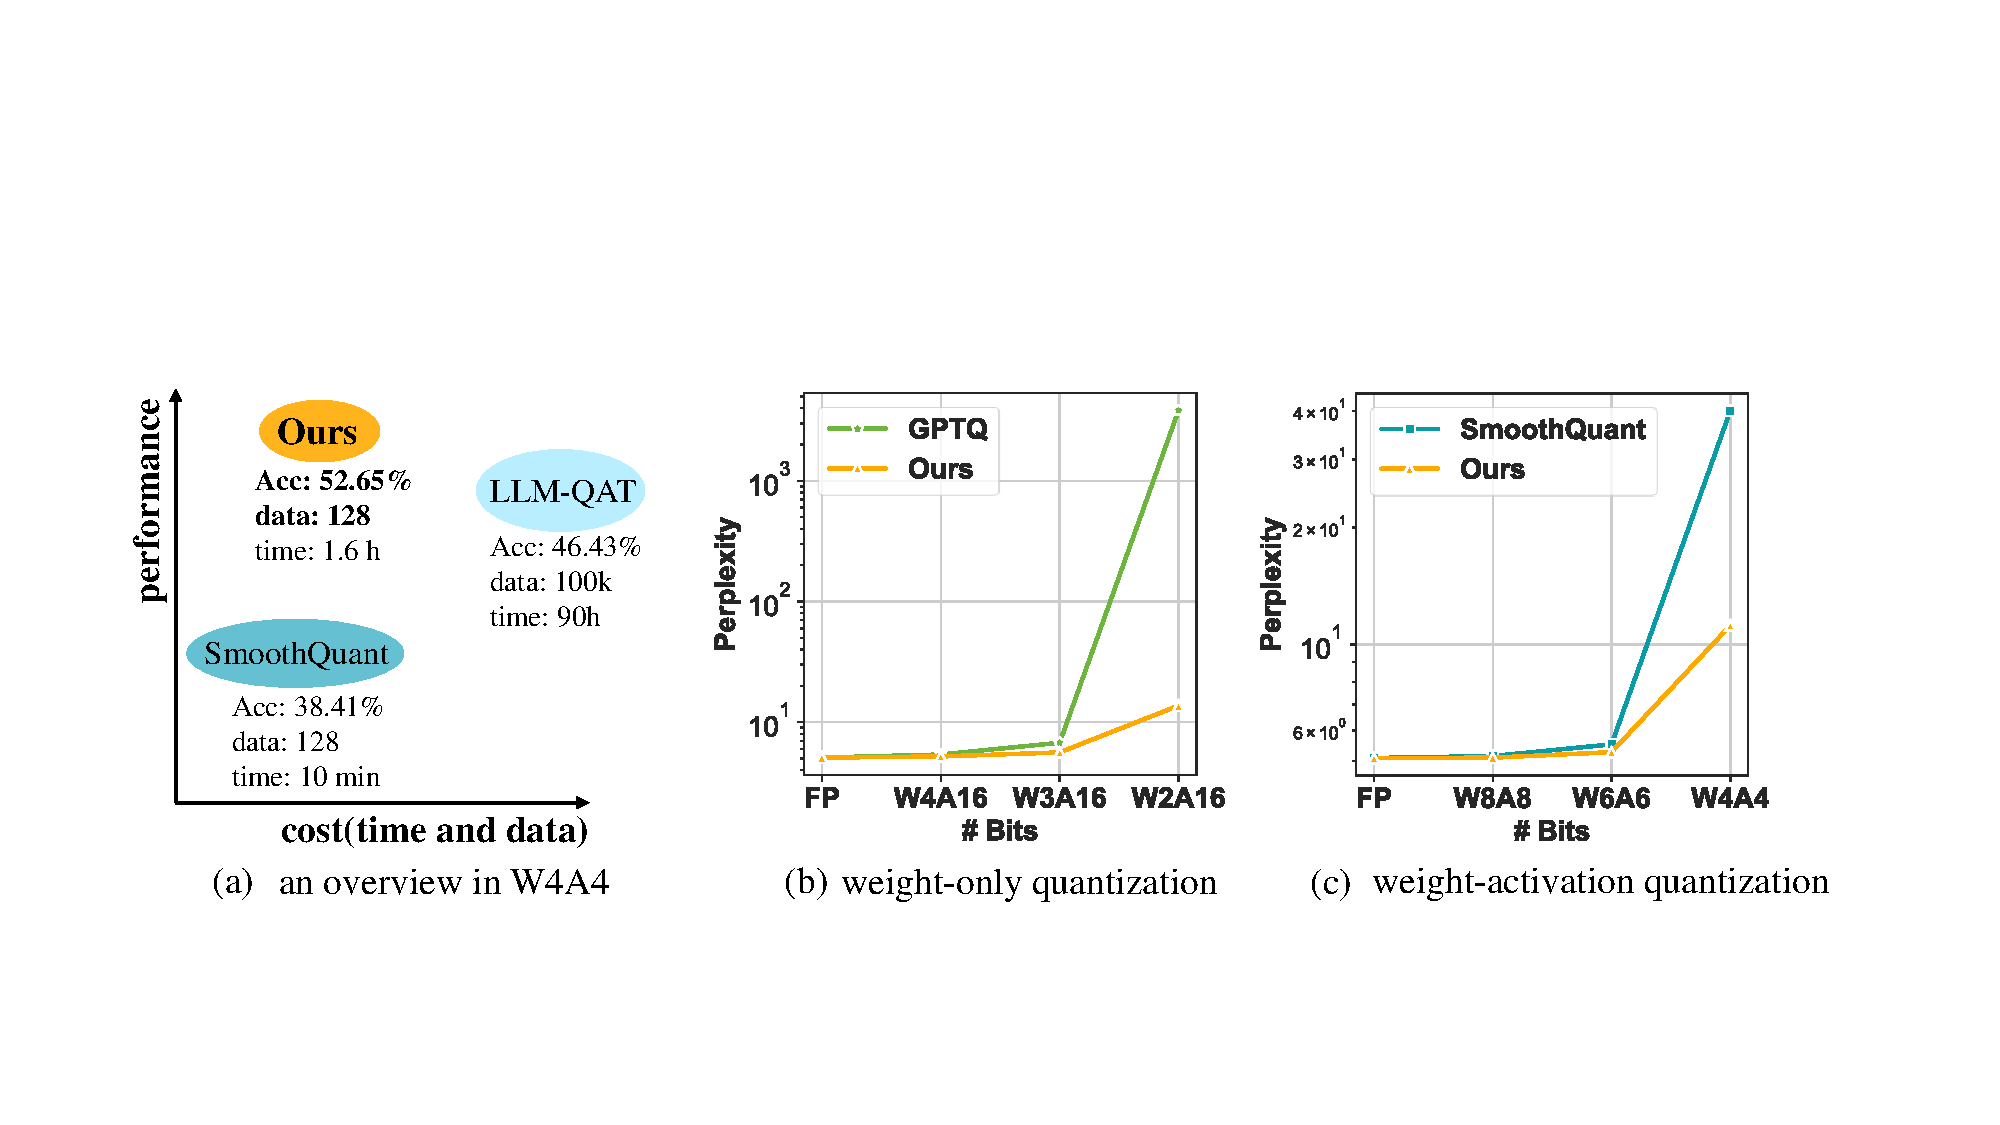
\includegraphics[width=0.85\textwidth]{teaser.pdf}
    \vspace{-0.15in}
    \caption{(a) provides an overview of LLaMA-7B with W4A4 quantization, highlighting OmniQuant's ability to achieve quantization-aware training (QAT) performance with post-training quantization (PTQ) time and data efficiency.  (b) and (c) showcase the perplexity (low is better) of quantized LLaMA-13B across different bit-widths on WikiText2.}
    \label{fig:teaser}
    \vspace{-2em}
\end{figure}

% Technical challenge for previous methods
Existing quantization methods have demonstrated significant achievements in various scenarios, including W4A16 (\emph{i.e.} 4-bit weight and 16-bit activation) weight-only quantization such as ~\citep{awq, spqr, owq}, as well as W8A8 weight-activation quantization~\citep{outlier-plus}.
%
However, they usually exhibit significant performance degradation when confronted with low-bit quantization, such as W2A16 and W4A4, as illustrated in Figure~\ref{fig:teaser} (b \& c).
%
This performance shortfall in low-bit quantization can be attributed to the fact that these methods~\citep{gptq,awq,outlier-plus} primarily rely on handcrafted quantization parameters such as migration strength \citep{smoothquant} and scaling parameters \citep{outlier-plus}, which often leads to lower performance.
%
Although Quantization-Aware Training (QAT) \citep{llmqat} is effective in determining the optimal quantization configurations, it introduces substantial training overhead in both training and data efficiency. It is thus hard to quantize LLMs with QAT-based techniques efficiently such as LLMQAT \citep{llmqat}. For instance, GPTQ~\citep{gptq}, a PTQ approach, can complete the quantization of LLaMA-13B in an hour using 128 samples on a single A100 GPU, while LLM-QAT~\citep{llmqat} requires 100k samples and hundreds of GPU hours.
%
This leads us to a central question: \emph{can we attain the performance of QAT, while maintaining the time and data efficiency of PTQ?}
%



% what we do






This paper introduces a novel quantization technique, OmniQuant, which effectively addresses the above question. OmniQuant achieves state-of-the-art performance across various quantization scenarios, particularly in low-bit settings, while preserving the time and data efficiency of PTQ, as illustrated in Figure \ref{fig:teaser}.
%
%The basic idea is illustrated in Figure~\ref{fig:teaser_method}.
%
Unlike Quantization-Aware Training (QAT)~\citep{llmqat} which involves cumbersome weight optimization, OmniQuant freezes the original full-precision weight and only incorporates a few learnable quantization parameters. 
%
As shown in Figure \ref{fig:teaser_method},
%
OmniQuant consists of two key components that incorporate different types of learnable quantization parameters, including Learnable Weight Clipping (LWC) and Learnable Equivalent Transformation (LET). Specifically, LWC modulates the extreme values of weights by optimizing the clipping threshold. In the meanwhile, LET tackles activation outliers by learning mathematically equivalent transformations in a transformer encoder.
%

Instead of jointly optimizing all parameters across the LLM, OmniQuant sequentially quantizes the parameters of one layer before moving on to the next under a block-wise quantization error minimization framework. 
%
In this way, 
OminiQuant can be optimized efficiently using a simple Stochastic Gradient Descent (SGD) algorithm. 
%
%This approach reduces the optimization difficulty and improves the quantization efficiency.
%
%
%
Thanks to the differentiable optimization, LWC and LET can be seamlessly integrated into the quantization.
We find that LWC can mitigate the difficulty in quantizing weights and LET further shifts the challenge of quantization from activations to weights, facilitating OmniQuant a versatile quantization framework for both weight-only and weight-activation quantization.
Notably, OmniQuant introduces no extra computation or parameters for the quantized model because the clipping threshold in LWC and equivalent factors in LET can be fused into quantized weights.
%
%These learnable parameters are responsible for transforming the original LLM from a quantization-hardly state into a quantization-friendly version.
%Specially, we present two innovative strategies: learnable weight clipping (LWC) and learnable equivalent transformation (LET), responsible for making weight and activation more quantization-friendly, respectively.
%Instead of learning the clipping threshold directly~\citep{lsq}, LWC forms the upper and lower bound threshold by scaling the maximum and minimum values respectively, ensuring that the clipping threshold remains within a meaningful range.
%The equivalent transformation indicates a manner that alters the distribution of intermediate weight and activation of models while without changing the final output.
%The LET strategy learns channel-wise scaling and shifting equivalent transformation to alleviate the impact of outliers~\citep{smoothquant,llmint8} within activations, thus reducing the challenges posed by activation quantization.
%We subsequently implement a block-wise calibration technique for the training of LWC and LET parameters. This indicates that only one transformer block in the LLM model is trained at a time, leading to significant memory savings for optimization.
%

\begin{wrapfigure}{r}{0.5\textwidth}
\vspace{-25pt}
\begin{center}
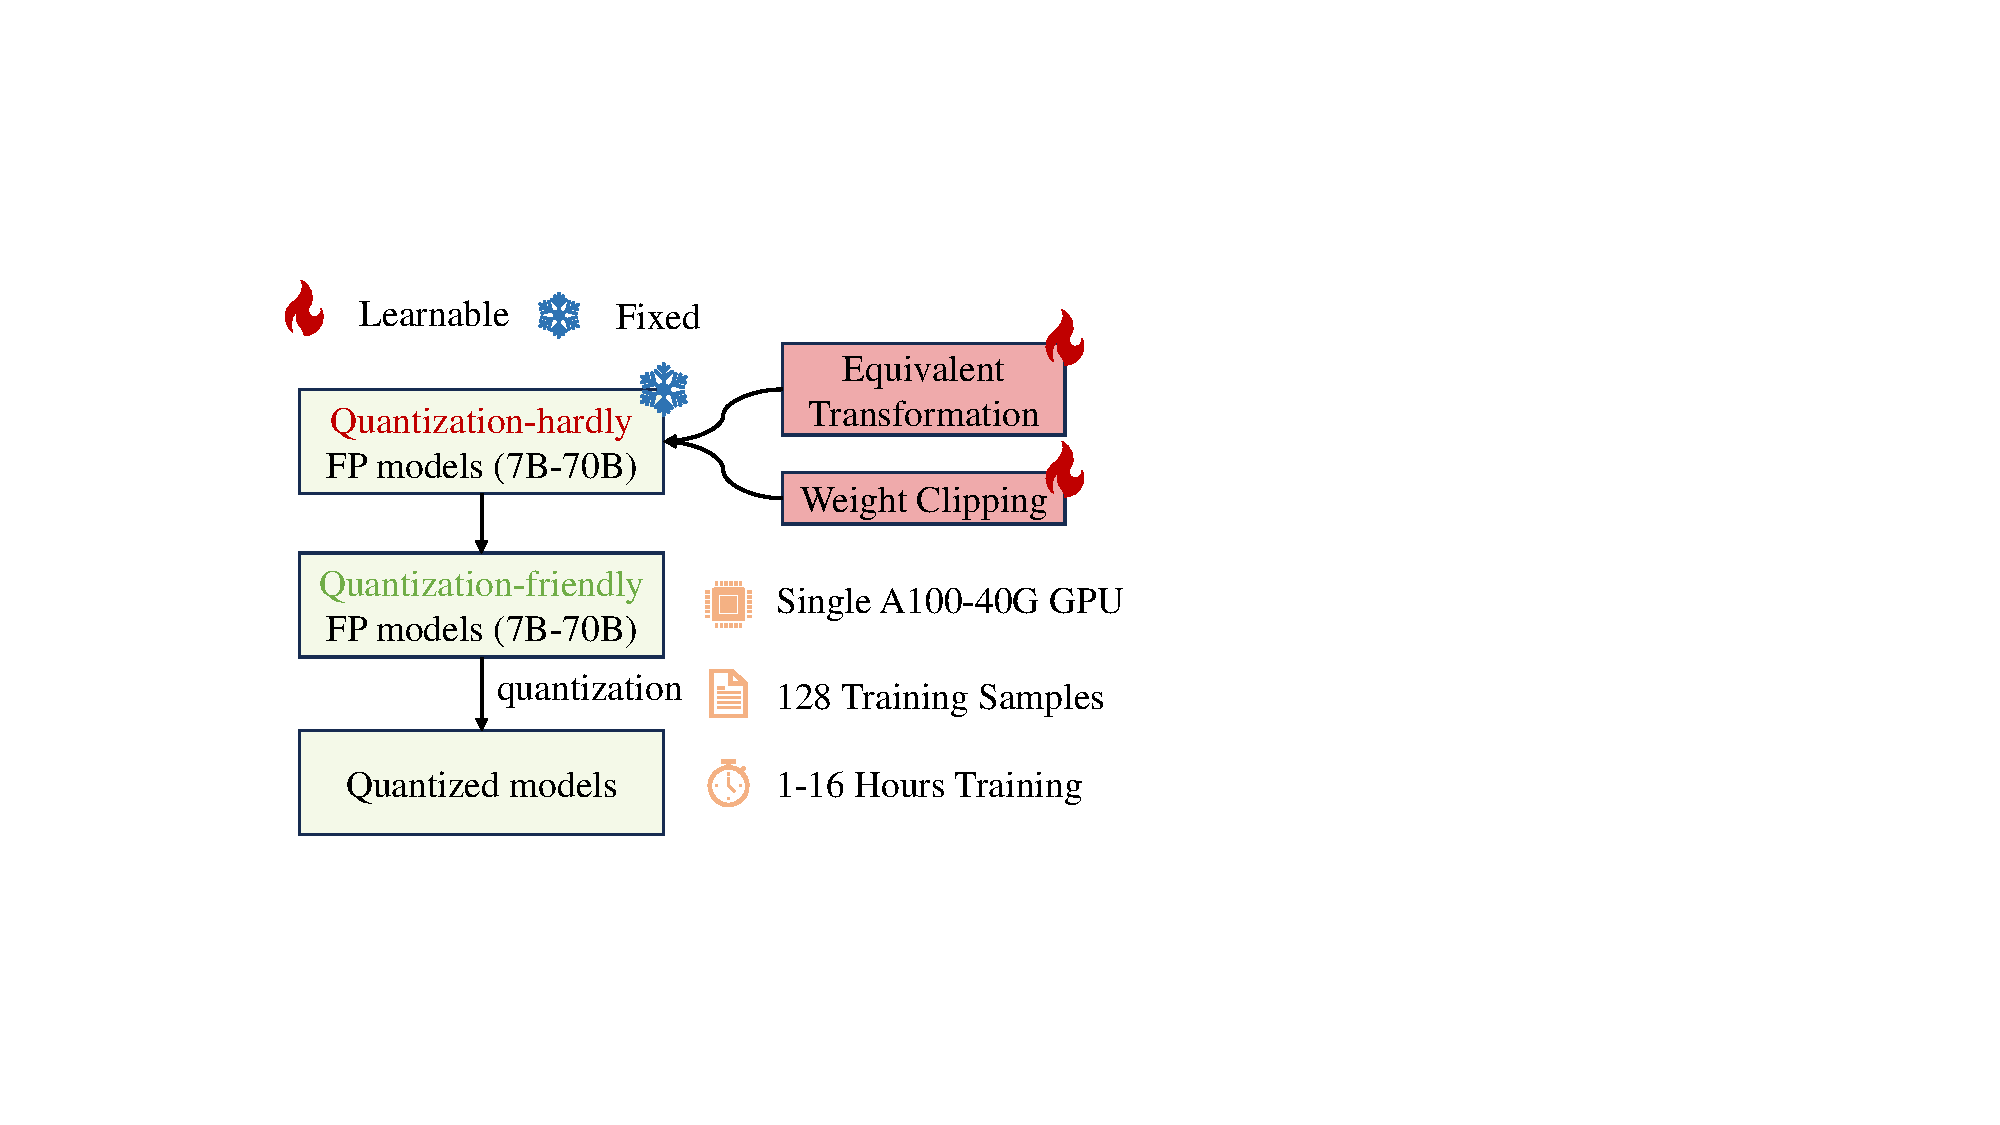
\includegraphics[width=0.45\textwidth]{teaser_method.pdf}
\vspace{-10pt}
\caption{Characteristics of OmniQuant on LLaMA family.}\label{fig:teaser_method}
\vspace{-10pt}
\end{center}
\end{wrapfigure}
% Experiments
As depicted in Figure~\ref{fig:teaser_method}, OmniQuant is easy to implement even with limited resources. Especially, taking the LLaMA-2 model family (7B-70B) as an example, all models can be quantized on a single A100-40G GPU utilizing only 128 training samples. The training time ranges from 1 to 16 hours, depending on the size of the quantized model, which ranges from 7B to 70B. 
%
Owing to the seamless integration of LWC and LET achieved by differentiable optimization, OmniQuant exhibits superior performance compared to prior PTQ-based methods in various quantization settings.  For example, when LLaMA-13B is quantized into W2A16, OmniQuant achieves a perplexity of $13.21$, while GPTQ incurs a significant increase in perplexity to $3832$, as demonstrated in Figure~\ref{fig:teaser}. A similar performance advancement is also observed in the W4A4 quantization.
%

% contribution
The contributions of \textbf{OmniQuant} are summarized as follows. 1) We formulate a novel quantization pipeline for LLM, OmniQuant, which freezes original full-precision weights while incorporating a restrained set of learnable parameters. OmniQuant imbues quantization with gradient updates while preserving the time and data efficiency of PTQ methods. 2) OmniQuant consists of Learnable Weight Clipping (LWC) and Learnable Equivalent Transformation (LET). These strategies make full-precision weights and activations more amenable to quantization.
3) Through extensive experiments, we demonstrate that OmniQuant outperforms previous methods across a spectrum of quantization settings (W416, W3A16, W2A16, W6A6, W4A4), various model families (OPT, LLaMA, LLaMA-2, LLaMA-2-chat, Falcon), and a range of model sizes (125M-180B). The computation speedup and memory reduction of OmniQuant are also demonstrated on real devices.









% \begin{figure}
%     \centering
%     
\includegraphics[width=\textwidth]{figures/teaser_method.pdf}
%     \caption{Characteristics of OmniQuant. OmniQuant effectively transforms full-precistion models from quantization-hardly into quantization-friendly through the application of learnable equivalent transfomation and learnable weight clipping. All OmniQuant experiments of  can be executed on a single A100-40G GPU and 128 training samples. The training time spans from 1 to 16 hours, contingent on the size of the quantized model, which ranges from 7B to 70B.}
%     \label{fig:teaser_method}
% \end{figure}

\section{Related Work}

\subsection{Quantization Methods.}
Quantization reduces neural network bit-precision, leading to smaller models and faster inference. Current methods are largely divided into Quantization Aware Training (QAT)\citep{llmqat} and Post-training Quantization (PTQ)\citep{smoothquant,gptq}. While QAT maintains performance by simulating quantization during training, its training cost makes it unsuitable for LLM. PTQ techniques like AdaRound~\citep{adaround} and BRECQ~\citep{brecq} use gradient optimization to determine optimal rounding, but tuning all weights is time-intensive for larger models. Thus, most LLM quantization methods~\citep{smoothquant,gptq,spqr,owq,outlier-plus} prioritize training-free PTQ, which limit performance in lower-bit situations. Our goal is to integrate gradient updates in LLM quantization, mirroring QAT's approach, while retaining PTQ's efficiency.

% Quantization compresses neural networks by reducing bit-precision, facilitating decreased model size and enhanced inference speed. Presently, quantization methods fall into two primary categories: Quantization Aware Training (QAT)~\citep{llmqat} and Post-training Quantization (PTQ)~\citep{smoothquant,gptq}. 
% By simulating quantization during training and searching optimal quantization parameters to minimize accuracy degradation, QAT helps preserve model performance even under lower-precision settings. However, it is impractical to use QAT in the context of LLM due to its significant training expense. Some PTQ techniques, such as AdaRound~\citep{adaround} and BRECQ~\citep{brecq}, employ gradient optimization and tune all weights to identify the optimal rounding operation in a data-efficient way. Nonetheless, adjusting all weights becomes time-consuming for models with billions of parameters. As a result, most extant quantization methods on LLMs~\citep{smoothquant,gptq,spqr,owq,outlier-plus} focus on training-free PTQ. However, the training-free method hinders the performance in the lower-bit scenario. In this work, we aim to incorporate gradient updates into LLM quantization like QAT while preserving the training time and data efficiency of PTQ.


% Quantization can be broadly classified into two main categories: \textbf{Quantization Aware Training}(QAT) and \textbf{Post Quantization Training}(PTQ), re-training full precision models and optimizing trained models respectively. The process of model quantization holds significance~\citep{deepcnn, nn, nn2, nlp} across neural networks (NN), deep neural networks (DNN), and Natural Language Processing(NLP) domains, and its facets can be dissected from various analytical perspectives. \textbf{Uniform Quantization}, which entails the conversion of continuous real-valued floating-point inputs into a discrete set of values via a rounding mechanism such as Round-to-Nearest (RTN). Additionally, the establishment of the clipping range may be accomplished through symmetric~\citep{symmetric} or asymmetric methodologies~\citep{asymmetric}. This quantization step assumes pivotal importance when addressing scenarios where there is an uneven distribution of target weights and activations. \textbf{Dynamic quantization} methods adopt a strategy of learn to compute the clipping range during the training process, thereby aiming to attain heightened accuracy levels. The concept of granularity pertains to the extent or scale at which the calculation of the clipping range is conducted. Specifically, three prominently adapted considerations in this realm are layerwise~\citep{gptq}, groupwise~\citep{shen2020q,zeroquant}, and channelwise~\citep{smoothquant} methodologies.

\subsection{Quantization of LLM.}
Considering the quantized object, exiting LLM quantization can be classified into two fields: weight-only quantization and weight-activation quantization. 

\textbf{Weight-only quantization.} Weight-only quantization focuses on converting weights to low-bit values. For instance, GPTQ~\citep{gptq} uses block-wise reconstruction for 3/4-bit quantization. SpQR~\citep{spqr}, OWQ~\citep{owq}, and AWQ~\citep{awq} emphasize the significance of weights tied to higher-magnitude activations.  Therefore, SpQR and OWQ employ mixed-precision quantization to safeguard vital weights, while AWQ opts for channel-wise scaling to avoid mixed-precision's hardware inefficiency. 
Qlora~\citep{qlora} and INT2.1~\citep{quip} restore the capabilities of the quantized model through parameter-efficient fine-tuning. Our method, in contrast, enhances the quantization process directly, making OmniQuant complementary to Qlora and INT2.1.

\textbf{Weight-activation quantization.} Weight-activation quantization compresses both weights and activations. SmoothQuant~\citep{smoothquant}, LLM.int8()~\citep{llmint8}, and Outlier Suppression~\citep{outlier} achieve W8A8 quantization by managing activation outliers. LLM.int8() uses mixed-precision decomposition, while the other two employ channel-wise scaling. Furthermore, Outlier Suppression+\citep{outlier-plus} adds channel-wise shifting to drive W6A6 quantization. Unlike previous heuristic designs, we use gradient optimization and expand equivalent transformations to attention mechanisms, further boosting the K/V cache quantization.
%
Recently, RPTQ~\citep{rptq} and LLM-QAT~\citep{llmqat} have achieved W4A4 quantization. However, RPTQ adopts deployment-unfriendly group-wise activation quantization, and LLM-QAT employs time-consuming QAT. In distinction from RPTQ and LLM-QAT, we achieve W4A4 quantization through deployment-friendly per-token quantization and maintain the PTQ efficiency.

% \textbf{Weight-only quantization.} Weight-only quantization exclusively converts weights into low-bit values.  For example, GPTQ~\citep{gptq} achieves 3/4-bit quantization using block-wise reconstruction. SpQR~\citep{spqr}, OWQ~\citep{owq}, and AWQ~\citep{awq} observe that weights related to activations of higher magnitude play a pivotal role in the final performance. Therefore, SpQR and OWQ safeguard these vital weights using mixed-precision quantization. In contrast, AWQ protects them via channel-wise scaling, circumventing the hardware inefficiency linked to mixed-precision quantization. Both Qlora~\citep{qlora} and INT2.1~\citep{quip} restore the capabilities of the quantized model through parameter-efficient fine-tuning. While our technique introduces additional learnable parameters, it differs fundamentally from Qlora and INT2.1. Specifically, Qlora and INT2.1 integrate learnable parameters post-quantization, whereas our approach aims to enhance the quantization process itself. Consequently, our proposed OmniQuant can be viewed as complementary to both Qlora and INT2.1.

% \textbf{Weight-activation quantization.} Weight-activation quantization compresses both weights and activations into low-bit values.  SmoothQuant~\citep{smoothquant}, LLM.int8()~\citep{llmint8}, Outlier Suppression~\citep{outlier} accomplish W8A8 quantization by addressing outlier issues in activations. In particular, LLM.int8() employs mixed-precision decomposition, segregating outlier feature dimensions into a 16-bit matrix multiplication. Both Outlier Suppression and SmoothQuant adopt channel-wise scaling to curtail outlier magnitudes. Furthermore, Outlier Suppression+~\citep{outlier-plus} integrates channel-wise shifting to further drive W6A6 quantization. 
% %
% Our approach also embraces channel-wise equivalent transformations. However, in contrast to heuristic designs~\citep{smoothquant,outlier,outlier-plus}, we utilize gradient optimization to determine the best solutions. We also extend equivalent transformations to attention mechanisms, not just confining them to linear layers,  enhancing the quantization of the K/V cache.
% %
% Recently, RPTQ~\citep{rptq} and LLM-QAT~\citep{llmqat} pushed the quantization levels down to W4A4. RPTQ segments activations into multiple groups according to clustering, subsequently employing group-wise activation quantization. LLM-QAT conducts data-free QAT, leveraging outputs generated by the pre-trained model. In distinction from RPTQ and LLM-QAT, we achieve W4A4 through deployment-friendly per-token quantization and maintain the PTQ efficiency.


% Quantization has emerged as a promising approach to reduce the computational cost of large language models (LLMs)~\citep{llmint8}. For instance, BERT, a widely used model in language inference and other natural language processing tasks~\citep{devlin2018bert}, has been successfully quantized for significant speedup~\citep{hou2020dynabert, kim2021bert,shen2020q}. However, as LLMs continue to scale up in size and face hardware limitations, these quantization methods encounter challenges in achieving relatively lossless performance at a reasonable cost.

% The practicality of Quantization-Aware Training (QAT) has diminished due to prohibitively high retraining costs associated with models of immense scale, such as OPT~\citep{zhang2022opt}, LLaMA ~\citep{llama},LLaMA-2~\citep{llama}and Bloom~\citep{scao2022bloom}, featuring 175B, 65B, and 176B parameters, respectively. Consequently, Post-Training Quantization (PTQ) has emerged as the predominant approach for addressing this challenge in the context of Language Models (LLMs). Compression outcomes can be classified into two categories: low-bit weight-only quantization and weight-and-activation quantization. Most state-of-the-art methods focus on addressing the precision issue through one of these aspects. For example, nuQmm~\citep{nuqmm} proposes group-wise binary-coding quantization on weights, which is a non-uniform quantization scheme enabling efficient quantized matrix multiplications. In practice, uniform quantization is extensively explored due to its simplicity in fixed-point operations. GPTQ~\citep{gptq} achieves 3 or 4 bits quantized weights by employing a layer-wise granularity quantization method with reconstruction. AWQ~\citep{awq} further enhances the model's generalization performance by omitting the backpropagation or reconstruction step, resulting in a 1.45× speedup over GPTQ. Regarding quantized activations, Zeroquant~\citep{zeroquant} and LLM.int8()~\citep{llmint8} are concurrent methods developed to reduce parameters to W8A8 with zero-degradation. However, zeroquant relies on layer-wise knowledge distillation, while LLM.int8() requires mixed INT8/FP16 decomposition. To further mitigate the additional overhead on memory and accelatare inference speed, Outlier suppression~\citep{outlier} introduces Gamma migration to alleviate the burden of activation quantization while minimally affecting weights. SmoothQuant~\citep{smoothquant} adapts channel-wise scaling factors to transfer activation difficulty to weights and conducts experiments on LLMs up to 176B in size. In LLA-QAT,~\citep{llmqat} additional trick such as knowledge distillation is adapted to perform data-free quantization training, pushing the limit to 4-bit weights, 4-bit KV cache and 8-bit activations. Unfortunately, existing methods either experience significant accuracy degradation when reducing the bitwidth below INT8 or lacking capacity for extremely large models. The most relevant work, smoothquant, does not sufficiently handel the inherent bottleneck in Transformer-based models, e.g.solely quantizes linear layers and retains some parameters at full precision in self-attention layers of transformers. An evaluation and comparison reveal that none of the existing methods achieves full accuracy recovery in weight-and-activation quantization~\citep{yao2023comprehensive}. Our proposed methods offer a universal approach to weight-only quantization (to W2A16) and weight-and-activation quantization (to W4A4), while also providing a quantization-friendly framework for self-attention layers in LLMs.
% \subsection{Adapter.}
% Adapters represent a modular component that integrates trainable parameters, enhancing the versatility and applicability of pre-trained language models for various downstream tasks. Extensive research has demonstrated the efficacy of adapter-based fine-tuning in terms of computational efficiency~\citep{ruckle2020adapterdrop} and effectiveness~\citep{he2021effectiveness}. This approach has also gained traction in domains beyond language processing, such as vision and multimodal tasks, including vision-and-language applications~\citep{sung2022vl}.
% The qLoRA~\citep{qlora} technique----Quantization and Low-Rank Adapter----specifically focuses on the quantization of language models. It freezes the original pre-trained weights to a 4-bit precision and subsequently fine-tuning additional low-rank adapters in a higher precision format. While this approach does reduce memory requirements, it introduces a relatively large number of additional parameters. Notably, other adapters, Quadapter~\citep{park2022quadapter} for GPT2, multi-model LLaMA-Adapter~\citep{llama-adapter}, and LLMs-Adapters~\citep{hu2023llm}, have been well developed. We propose a novel technique called OmniQuant, which aims to facilitate both weight and activation quantization while preserving the model's generalization capabilities. By enhancing the quantization-friendliness of both weights and activations, our method seeks to strike a balance between efficient memory utilization and overall model performance.

\iffalse
\section{Preliminaries}
Let us begin with briefly introducing several representative quantization schemes for LLMs.

\textbf{Post-Training Quantization (PTQ).} Due to the high computation and data efficiency, PTQ-based methods are widely used to compress LLMs. Considering the fact that there are a few outlier channels in the original activation map while the original weight distribution is flat and uniform, SmoothQuant \citep{smoothquant} and Outlier Suppression+ \citep{outlier-plus} conduct weight-activation quantization by migrating the quantization difficulty from activations to weights with a pre-defined migration strength. In addition, another line of work finds that the quantization error of weights also plays a pivotal role in the final performance due to the importance of weights corresponding to activations. To overcome this, SqQR \citep{spqr} and OWQ \citep{owq} retain crucial weights in full-precision, while AWQ \citep{awq} safeguards these weights using grid-searched channel-wise scaling.

\textbf{Challenge of LLM quantization.} Although these methods have achieved certain success in compressing various LLMs, they often lead to suboptimal performance and fail to deal with extremely low-bit quantization due to the crude design of quantization parameters.
%



%As discussion in existing  works\citep{llmint8,smoothquant}, there are a few outlier channels in the original activation map, while the original weight distribution is flat and uniform.
% Activation
%Therefore, several works\citep{llmint8,smoothquant,outlier-plus} focus on alleviate outlier problems to impel activation quantization. For example, SmoothQuant \citep{smoothquant} conducts weight-activation quantization by migrating the quantization difficulty from activations to weights with a pre-defined migration strength. Moreover, Outlier Suppression+ \citep{outlier-plus} quantitatively analyzes the appropriate values for shifting and scaling parameters in quantization. Although these methods have achieved certain success, they often lead to suboptimal performance and fail to deal with extremely low-bit quantization due to the crude design of quantization parameters.


%Recent PTQ-based quantization methods simplify LLM quantization by hand-crafting quantization parameters. For example, 
% Weight


\textbf{Technical Challenges.}


Quantization maps float-point values into low-bit values, resulting in significant memory save and inference speedup.
%
In this work, we study linear quantization because of its deploy-friendly properties. Also, we investigate block-wise optimization to minimize the quantization error.
%Also, we leverage fine-grain quantization schemes to push the quantization of LLM into lower bits.
% \subsection{Linear Quantization}

\textbf{Linear quantization}, \emph{i.e.}, uniform quantization, can be formulated as:
\begin{equation}\label{eq:quantization}
    \mathbf{X_q} = \mathrm{clamp}(\lfloor \frac{\mathbf{X}}{s} \rceil + z, 0, 2^{N}-1),
\end{equation}
where $\lfloor \cdot \rceil$ indicates round operation. $N$ is the target bit number. $\mathbf{X}_q$ and $\mathbf{X}$ denote the quantized and full-precision items, respectively. $s$ is the scaling factor and $z$ is the zero-point value. The clamp operation constrains the value within the range of $N$-bit integer, specifically $[0, 2^{N}-1]$.
%assigns each weight to the nearest quantization level from $0$ to $2^N-1$.
%
For instance, MinMax quantization~\citep{smoothquant} is a widely-used linear quantization scheme, which restrains quantized weights within the minimum and the maximum of full-precision weights. To this end, MinMax quantization typically sets $s={\max(\lvert \mathbf{X} \rvert)}/{(2^{N-1}-1)}, z=2^{N-1}-1$ for symmetric quantization and sets $s=[\max(\mathbf{X})-\min(\mathbf{X} )]/{(2^{N}-1)}, z=-\lfloor {\min(\mathbf{X})}/{s} \rceil$ for asymmetric quantization.

%preserves all value ranges. Therefore, MinMax quantization obtains $s$ and $z$ through the maximum and minimum values. For symmetric quantization, $s=\frac{\max(\lvert \mathbf{X} \rvert)}{2^{N-1}-1}, z=2^{N-1}-1$. And for asymmetric quantization, $s=\frac{\max(\mathbf{X})-\min(\mathbf{X} )}{2^{N}-1}, z=-\lfloor \frac{\min(\mathbf{X})}{s} \rceil$.

%Considering whether clip the real value, linear quantization can be categorized into two types: 
% \textbf{Clipping-based quantization} clips the outliers to allocate more bits to the intermediate values. Indeed, the clipping can be realized by adjusting scaling factor $s$ and zero-point value $z$.
% $s$ and $z$ can be obtained in many ways, such as grid searching~\citep{awq}, statistics~\citep{statsq}, and gradient update~\citep{statsq}.

\textbf{Post-Training Quantization (PTQ).} 

The traditional PTQ methods~\citep{gptq,adaround,brecq,qdrop} tune the full weights with minor modifications by block-wise quantization error minimization, which can be formulated as:
\begin{equation}\label{eq:deltaW-PTQ}
    \arg\min_{\Delta\mathbf{{W}}} \lvert\lvert \mathbf{F}(\mathbf{W},\mathbf{X}) - \mathbf{F}\big(Q_w(\mathbf{W}+\Delta\mathbf{{W}}),Q_a(\mathbf{X})\big) \rvert\rvert,
\end{equation}
where $\mathbf{F}$ represents the function of a layer~\citep{gptq,adaround} or a block~\citep{brecq,qdrop}. $\mathbf{W},\Delta\mathbf{{W}}$ denote the original weights and minor weights modification, respectively. $\mathbf{X}$ denotes the input activation corresponding to a small calibration dataset. $Q_w(\cdot)$ and $Q_a(\cdot)$ represent weight and activation quantizer, respectively. 
Despite the fact that block-wise minimization reduces the memory footprint, the traditional PTQ methods cannot be directly used to quantize LLM due to the heavy computational overhead of updating billions of parameters.
\fi
%
%Recent PTQ-based quantization methods simplify LLM quantization by hand-crafting quantization parameters. For example, SmoothQuant \citep{smoothquant} conducts weight-activation quantization by migrating the quantization difficulty from activations to weights with a pre-defined migration strength. Moreover, Outlier Suppression+ \citep{outlier-plus} quantitatively analyzes the appropriate values for shifting and scaling parameters in quantization. Although these methods have achieved certain success, they often lead to suboptimal performance and fail to deal with extremely low-bit quantization due to the crude design of quantization parameters.

% The quantization process of MinMax quantization can be formulate as:
% \begin{equation}
% \mathbf{X}_q = s\lfloor \frac{\mathbf{X}}{s} + z \rceil - z,
% \end{equation}
% where $\lfloor \cdot \rceil$ indicates round. $\mathbf{X}_q$ and $\mathbf{X}$ denote the quantized and full-precision items, respectively. $s$ is the scaling factor and $z$ is the zero-point value. Given $N$-bits, $s=\frac{\max(\lvert \mathbf{X} \rvert)}{2^{N-1}-1}, z=0$ for symmetric quantization, and $s=\frac{\max(\lvert \mathbf{X} \rvert)}{2^{N}-1}, z=-\lfloor \frac{\min(\mathbf{X})}{s} \rceil$ for symmetric quantization.


% \subsection{Fine-grain Quantization}
% Fine-grain Quantization indicates reduce the quantization error by introducing more quantization parameters, realized by dividing the quantized objects into multiple groups and equiping each group values with individual quantization parameters ($s$ and $z$).
% %
% Through fine-grain quantization, performance of low-bit models can be significantly improve~\citep{qlora,llmint8,frantar2022gptq,dettmers2023case}. In this work, we leveraging vector-wise quantization~\citep{llmint8} for weight-activation quantization and group-size quantization~\citep{nuqmm} for weight-only quantization.

% \textbf{Vector-wise Quantization.}
% Given 

% \textbf{Group-wise quantization.}
% Given the weight matrix $\mathbf{W} \in \mathbb{R}^{C_{in}\timesC_{out}}$




\begin{figure}[!t]
    \centering
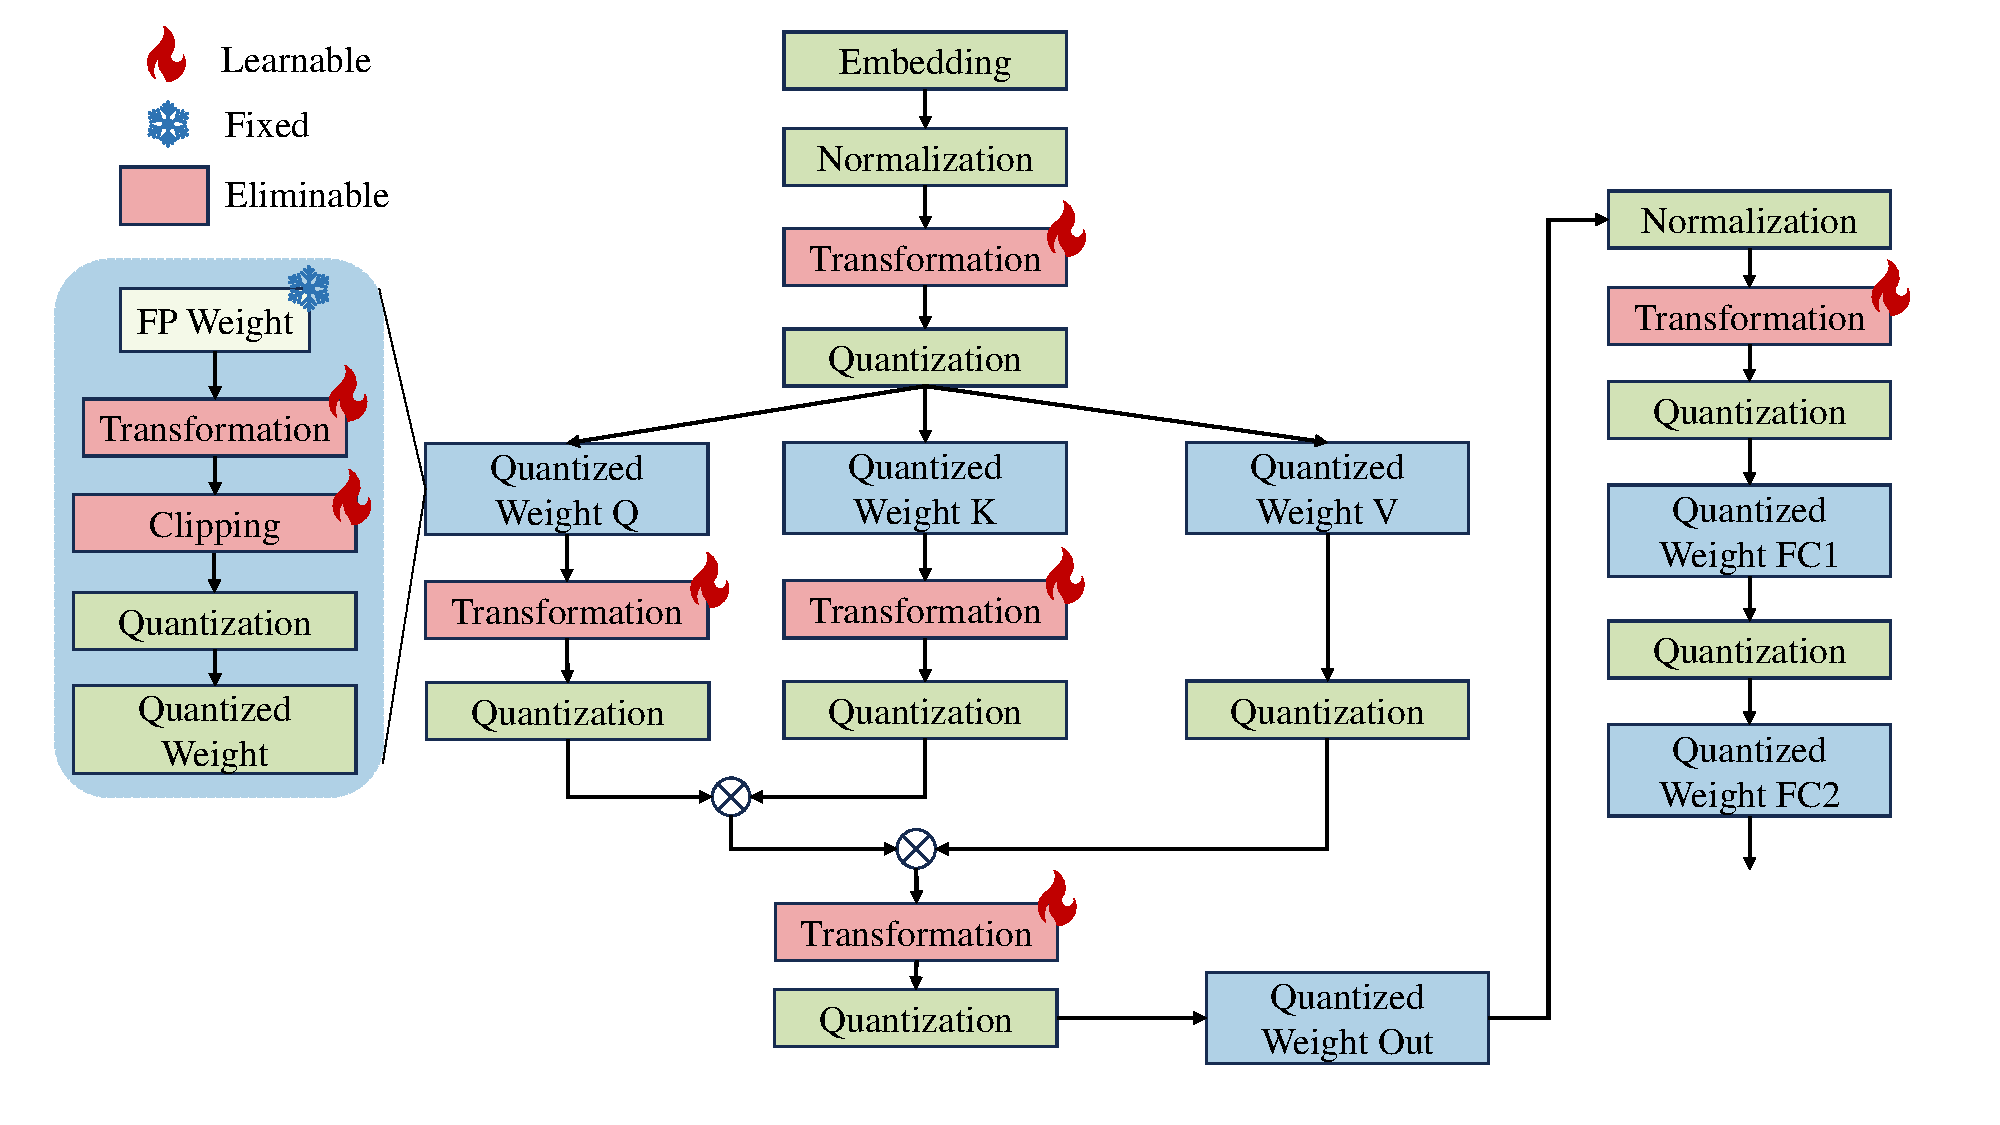
\includegraphics[width=0.7\textwidth]{framework.pdf}
\vspace{-1em}
    \caption{\textbf{Details of OmniQuant} in a transformer block. Note that all learnable parameters can be eliminated after quantization.}\label{fig:framework}
    \vspace{-1.5em}
\end{figure}

\section{OmniQuant}



% \begin{figure}
%     \centering
%     \includegraphics[width=\textwidth]{equivalent transformation.pdf}
%     \caption{\textbf{OmniQuant examples.} Each equivalent transformation adapter consists of a transformation operation and an inverse transformation operation. (a) demonstrates the usage of OmniQuant in a linear layer, enhancing the quantization compatibility of input feature $X$ and weight $W$. (b) illustrates the application of OmniQuant in a self-attention operation, improving the quantization compatibility of the query/key/value vectors $Q$/$K$/$V$. The bias of the linear layer is omitted for clarity in the representation.}
%     \label{fig:framework}
% \end{figure}
\textbf{Challenge of LLM quantization.} Two main difficulties lie in quantizing an LLM. First, the activation is hard to quantize due to the existence of outlier channels.  Considering that weight distribution is flat and uniform, SmoothQuant \citep{smoothquant} and Outlier Suppression+ \citep{outlier-plus} tackle this issue by migrating the quantization difficulty from activations to weights with a pre-defined migration strength or grid-searching based optimization. Second, the quantization error of weights also plays a pivotal role in the final performance due to the importance of weights corresponding to activations. SqQR \citep{spqr} and OWQ \citep{owq} propose to retain crucial weights in full-precision, while AWQ \citep{awq} safeguards these weights using grid-searched channel-wise scaling.  Although these methods have achieved certain success in compressing various LLMs, they often lead to suboptimal performance and fail to deal with extremely low-bit quantization due to the crude design of hand-crafted quantization parameters such as migration strength and scaling factors.
%

In this section, we introduce a differentiable quantization technique for LLM called \textbf{OmniQuant} where quantization parameters are learned with better flexibility. Towards this goal, OmniQuant is implemented with a block-wise quantization error minimization framework as presented in Sec.\ref{sec:method-blockwise-minimization}. To tackle the aforementioned challenges of LLM quantization, we devise two novel strategies for additional learnable quantization parameters including a learnable weight clipping (LWC) to mitigate the difficulty in quantizing weights and a learnable equivalent transformation (LET) to further shift the challenge of quantization from activations to weights. We introduce LWC and LCT in Sec. \ref{sec:LWC} and Sec. \ref{sec:LET}, respectively.



\iffalse
we introduce a novel optimization pipeline, which freezes the original full-precision weight parameters but optimizes a few quantization parameters within the block-wise quantization error minimization framework.
%Optimizing all weight parameters is prone to overfitting the calibration dataset and leading to too slow convergence.
%
To tackle this, we first introduce a novel optimization pipeline, which freezes the original full-precision weight parameters but introduces a limited set of learnable parameters.
%
The learnable parameters can be used to translate the quantized model, leading to more quantization-friendly weights and activations.
%
Specifically, we devise two novel strategies for additional learnable parameters: learnable weight clipping (LCT) and learnable equivalent transformation (LET).
%
The former LCT facilitates weight quantization by adaptively clipping each quantization group, achieving appropriate quantization precision trade-off between outlier and regular weights.
%
The later LET alleviates the quantization challenges posed by outlier activation through learnable channel-wise scaling and shifting.
%
With the cooperation of LCT and LET, the proposed OmniQuant can realize Omni-bearing quantization, encompassing both weight-only quantization and weight-activation quantization.
%
The details of OmniQuant are illustrated in Figure~\ref{fig:framework}. Additionally, the comprehensive training algorithm of OmniQuant is illustrated in Algorithm\,\ref{alg:omniquant} in Appendix.
\fi

\subsection{Block-wise Quantization Error Minimization}\label{sec:method-blockwise-minimization}
Previous PTQ methods with gradient optimization, such as AdaRound~\citep{adaround}, BRECQ~\citep{brecq} cannot be applied in models with billions of parameters because they are hard to optimize due to the huge solution space. 
%Moreover, current gradient optimization methods focus on reducing the reconstruction error by learning the weight-rounding mechanism, while omitting the difficulty of activation quantization. 
%
Instead of turning the whole model, we propose a new optimization pipeline with block-wise quantization error minimization where the additional quantization parameters can be optimized in a differentiable manner. We formulate the optimization goal as follows:
\begin{align}
\arg \min_{\Theta_1, \Theta_2} \lvert\lvert \mathcal{F}(\mathbf{W},\mathbf{X}) - \mathcal{F}\big(Q_w(\mathbf{\mathbf{W}}; \Theta_1,\Theta_2),Q_a(\mathbf{X}, \Theta_2)\big) \rvert\rvert, 
\label{eq:objective}
\end{align}
where $\mathcal{F}$ represents the mapping function for a transformer block in the LLM, $\mathbf{W}$ and $\mathbf{X}$ are full-precision weight and activation, $Q_w(\cdot)$ and $Q_a(\cdot)$ represent weight and activation quantizer, respectively, $\Theta_1$ and $\Theta_2$ are quantization parameters in learnable weight clipping (LWC) and learnable equivalent transformation (LET), respectively. The Block-wise quantization in Eqn.(\ref{eq:objective}) sequentially quantizes the parameters of one transformer block before moving on to the next.

Block-wise minimization in Eqn.(\ref{eq:objective}) has two advantages. First, equipped with block-wise minimization in Eqn.(\ref{eq:objective}), OmniQuant can optimize quantization parameters in LWC and LET jointly, making it capable enough to encompass both weight-only and weight-activation quantization. Second, block-wise minimization is easy to optimize with minimal resource requirements. OmniQuant only determines a few quantization parameters with optimality, which is easier than optimizing the whole weights in previous PTQ-based methods \citep{adaround, brecq}. Empirically, we find that all models from the LLaMA-2 family \citep{llama2} can be quantized on a single A100-40G GPU utilizing only 128 training samples.

%In this study, $\theta$ includes learnable weight clipping (Sec.\,\ref{sec:LWC}) and learnable equivalent transformation(Sec.\,\ref{sec:LET}).


% \begin{wraptable}{r}{0.38\textwidth}
% \vspace{-21pt}
% \centering
% \begin{tabular}{cc}
% \hline
% Method & Perplexity \\
% \hline
% FP & 5.68 \\
% MinMax & 25.73 \\
% PACT~\citep{pact} & 6.95\\
% LSQ~\citep{lsq} & \\
% LWC (Ours) & \textbf{6.47} \\
% \hline
% \end{tabular}
% \vspace{-10pt}
% \caption{WikiText2 perplexity of clipping-based quantization methods in W3A16 LLaMA-7B.}
% \label{tab:clipping_method}
% \vspace{-13pt}
% \end{wraptable}

\subsection{Learnable Weight Clipping}\label{sec:LWC}
% Motivation
OmniQuant employs a module of learnable weight clipping (LWC) to reduce the difficulty of quantizing the weights in an LLM. Similar to previous methods with learnable clipping threshold~\citep{lsq,statsq,pact}, LWC also determines the optimal dynamic range of the weights by optimizing a clipping threshold. However, we find that directly employing prior arts such as PACT \citep{pact} and LSQ \citep{lsq} in quantization would produce unsatisfactory performance, as demonstrated in Table\,\ref{tab:clipping_method} in the Appendix.


Instead of directly learning a clipping threshold as in previous methods \citep{lsq,pact}, LWC optimizes a clipping strength as formulated by
\begin{equation}\label{eq:LWC}
    \mathbf{W_q} = \mathrm{clamp}(\lfloor \frac{\mathbf{W}}{h} \rceil + z, 0, 2^{N}-1), \mathrm{where}\,\, h=\frac{\gamma\max(\mathbf{W})-\beta\min(\mathbf{W} )}{2^{N}-1}, z=-\lfloor \frac{\beta\min(\mathbf{W})}{h} \rceil
\end{equation}
where $\lfloor \cdot \rceil$ indicates round operation. $N$ is the target bit number. $\mathbf{W}_q$ and $\mathbf{W}$ denote the quantized and full-precision weights, respectively. $h$ is the normalization factor for weights and $z$ is the zero-point value. The clamp operation constrains the value within the range of $N$-bit integer, specifically $[0, 2^{N}-1]$. In Eqn.(\ref{eq:LWC}), $\gamma\in[0,1]$ and $\beta\in[0,1]$ are learnable clipping strengths for the upper and the lower bound of weights, respectively. We instantiate $\gamma$ and $\beta$ by the sigmoid function\footnote{$\mathrm{Sigmoid}(t)=1/(1+\exp^{-t})$}. Hence, $\Theta_1=\{\gamma,\beta\}$ in Eqn.(\ref{eq:objective}).
%We instantiate them by $\gamma=1/(1+\exp^(-\gamma_0)$ and $\beta=1/(1+\exp^(-\beta_0)$ where $\gamma_0$ and $\beta_0$ are learnable parameters.

Note that LWC degrades into a vanilla MinMax quantization scheme used in existing works \citep{smoothquant},\cite{gptq} when $\gamma=1$ and $\beta=1$. 
%
%Our proposed LWC has two advantages compared with prior methods. First, LWC degrades into a vanilla MinMax quantization scheme used in SmoothQuant\cite{smoothquant} when $\gamma=1$ and $\beta=1$. 
By inheriting the benefits of MinMax quantization, LWC only needs to adjust the clipping strengths to determine an optimal clipping threshold, which would reduce the optimization difficulty.
%Hence, LWC reduces the optimization difficulty in determining an optimal clipping threshold by inheriting the benefits of MinMax quantization. 
Clipped by an optimal threshold, the original weights would be easy to quantize.
%
As indicated by the experiments in Table\,\ref{tab:llama_weight_only}, our proposed learnable weight clipping method significantly outperforms previous weight-only quantization techniques~\citep{gptq,awq}).
%MinMax quantization treats all weights equally, but it is intuitive that different weights contribute variedly to the final outputs~\citep{wanda,awq}).
%
%A classical way to improve MinMax quantization involves clipping-based quantization, which adjusts the clipping threshold to strike a balance in quantization precision between outliers and regular values. 
%
\iffalse
However, the direct application of the previous methods~\citep{lsq,statsq,pact} into LLMs produces worse performance than Min-Max quantization, as demonstrated in  LLM-QAT~\citep{llmqat}. A similar result has been also observed in Table\,\ref{tab:clipping_method} in the Appendix.
%Table.{\color{red}{TODO}}. A similar observation has also been made in LLM-QAT~\citep{llmqat}.

%
The failure of previous methods in LLM can be attributed to two main factors. First, these methods directly learn the clipping threshold or step size, which creates a vast solution space and poses a significant convergence challenge. Second, outliers~\citep{llmint8} in activation significantly affect the final output, rendering the activation unsuitable for clipping operations.
%



To address these issues, we focus on weight clipping and propose a novel learnable weight clipping method, which obtains the clipping threshold by scaling the original minimum and maximum values. 
%
Specifically, for each quantization group, we introduce two learnable parameters, $\gamma_{max}$ and $\gamma_{min}$, representing the maximum and minimum clipping scales, respectively. Additionally, a sigmoid function is employed to limit the clipping scale within the meaningful range $[0,1]$. This process can be formulated as follows:
\begin{equation}
    \hat{\alpha}_{max} = \mathrm{Sigmoid}(\gamma_{max}) \cdot \alpha_{max}, \hat{\alpha}_{min} = \mathrm{Sigmoid}(\gamma_{min}) \cdot \alpha_{min},\label{eq:clipping_scale}
\end{equation}
where $\alpha_{max} = max(\mathbf{W}), \alpha_{min} = min(\mathbf{W})$ represents the original maximum and minimum values within the quantization group, while $\hat{\alpha}_{max}$ and $\hat{\alpha}_{min}$ denote the upper bound and lower bound for clipping operation.
%
In our experiments, we init $\gamma_{max}=\gamma_{min}=4$, resulting $0.98$ after $\mathrm{Sigmoid}$. Such initialization can ensure that most information is preserved at the learning start point and avoid the gradient disappearance problem when $\mathrm{Sigmoid}$ meets the saturated zone.
%
After weight clipping with clipping threshold $\hat{\alpha}_{max}$ and $\hat{\alpha}_{min}$ in Eq.(\ref{eq:clipping_scale}), the scaling factor $s$ and zero-point value $z$ for quantization are calculated similarly as in MinMax quantization, based on the clipped weights:
\begin{equation}
    s = \frac{\hat{\alpha}_{max}- \hat{\alpha}_{min}}{2^N - 1}, z=\frac{\hat{\alpha}_{min}}{s}.\label{eq:clipping_sz}
\end{equation}
Both $s$ and $z$ influence all weights, thereby enabling the gradient of all weights to propagate to the learnable $\gamma_{max}$ and $\gamma_{min}$.  

Our proposed learnable clipping has two key advantages. First, it can be seen as constructing clipping-based quantization by using MaxMin quantization as a proxy, thereby limiting the solution space to meaningful domains.
%
Second, as indicated by the experiments in Table\,\ref{tab:llama_weight_only}, our proposed learnable weight clipping method significantly outperforms previous weight-only quantization techniques~\citep{gptq,awq}.
\fi

\subsection{Learnable Equivalent Transformation}\label{sec:LET}
% Motivation
Other than LWC which enables quantization-friendly weights by optimizing the clipping threshold, we further reduce the difficulty of weight-activation quantization by a learnable equivalent transformation (LET). 
%
Considering that outliers in the activation map are systematic and unique to specific channels, previous methods such as SmoothQuant \citep{smoothquant} migrate the difficulty of quantization from activations to weights with a mathematically equivalent transformation. However, they hand-craft the equivalent parameters, leading to suboptimal results.

Thanks to the inclusion of block-wise quantization error minimization, our LET can determine the optimal equivalent parameters in a differentiable way. 
%
Inspired by SmoothQuant~\citep{smoothquant} and Outlier Suppression+~\citep{outlier-plus}, we adopt channel-wise scaling and channel-wise shifting to manipulate the activation distribution, providing an effective solution for the outlier issue.
%
Specifically, we investigate the equivalent transformation across both the linear layer and attention operation, as illustrated in Figure\ref{fig:framework}.

\textbf{Linear layer.} The linear layer takes an input token sequence $\mathbf{X} \in \mathbb{R}^{T\times C_{in}}$ where $T$ is the token length and is the multiplication of the weight matrix $\mathbf{W} \in \mathbb{R}^{C_{in} \times C_{out}}$ and bias vector $\mathbf{B}\in\mathbb{R}^{1 \times C_{out}}$. A mathematically equivalent linear layer is expressed as:
\begin{equation}\label{eq:original_linear}
    \mathbf{Y} = \mathbf{X}\mathbf{W} + \mathbf{B} = [\underbrace{(\mathbf{X}-\delta)\oslash s}_{\tilde{\mathbf{X}}}]\cdot[\underbrace{s\odot \mathbf{W}}_{\tilde{\mathbf{W}}}] + [\underbrace{\mathbf{B} + \delta\mathbf{W}}_{\tilde{\mathbf{B}}}]
    %Q_x(\mathbf{X}) Q_w(\mathbf{W}) + \mathbf{B}. 
\end{equation}
where $\mathbf{Y}$ represents the output,  $\mathbf{s} \in \mathbb{R} ^{1\times C_{in}}$ and $\mathbf{\delta} \in \mathbb{R}^{1\times C_{in}}$ are channel-wise scaling and shifting parameters, respectively, $\tilde{\mathbf{X}}, \tilde{\mathbf{W}}$ and $\tilde{\mathbf{B}}$ are equivalent activation, weight and bias, respectively, `$\oslash$' and `$\odot$' are elementwise division and multiplication. By Eqn.(\ref{eq:original_linear}), the activations are transformed to be quantization-friendly at a cost of increased quantization difficulty in weights. In this sense, LWC in Sec. \ref{sec:LWC} can improve the performance of weight-activation quantization achieved by LET because it renders weights quantization-friendly. Finally, we perform quantization on transformed activations and weights, as given by
%
\begin{equation}\label{eq:LET-linear}
    \mathbf{Y} = Q_a(\tilde{\mathbf{X}}) Q_w(\tilde{\mathbf{W}}) + \widetilde{\mathbf{B}},
\end{equation}
where $Q_a$ is the vanilla MinMax quantizer and $Q_w$ is the MinMax quantizer with learnable weight clipping (i.e. our LWC).

Note that the scaling and shifting parameters in $\tilde{\mathbf{X}}$ can be absorbed into the previous normalization or linear layer and the the scaling factors in $\tilde{\mathbf{W}}$ can be fused into the original linear weight $\mathbf{W}$. Therefore, the equivalent transformation in Eqn.(\ref{eq:original_linear}) can effectively reduce quantization errors without introducing additional parameters or costs. We employ this equivalent transformation in all linear layers of the LLM except for the second linear layer of FFN as shown in Figure\ref{fig:framework}. This may be because the high sparsity of features after the non-linear layer~\citep{dejavu} leads to unstable gradients when applying learnable equivalent transformations.



\textbf{Attention operation.} Beyond the linear layer, the attention operation also accounts for a significant proportion of the computation. Additionally, the auto-regressive pattern of LLM necessitates storing the key-value(KV) cache for each token, which results in substantial memory demands for long sequences. Therefore, we also quantize $\mathbf{Q}/\mathbf{K}/\mathbf{V}$ matrixes into low-bit in the weight-activation quantization setting. Specifically, the learnable equivalent transform of the self-attention affinity matrix can be written as:
\begin{equation}\label{eq:LET-attn}
    \mathbf{P} =\mathrm{Softmax} (\mathbf{Q} \mathbf{K} ^{T})=\mathrm{Softmax} ((\underbrace{\mathbf{Q}\oslash s_a}_{\tilde{\mathbf{Q}}}) (\underbrace{s_a\odot\mathbf{K} ^{T}}_{\tilde{\mathbf{K}}^T})).
\end{equation}
where $s_a\in \mathbb{R}^{1\times C_{out}}$ is the scaling factor in the affinity matrix. Similar to Eqn.(\ref{eq:LET-linear}), the quantized affinity matrix calculation is expressed as $\mathbf{P} = \mathrm{Softmax} (Q_a (\widetilde{\mathbf{Q}}) Q_a (\widetilde{\mathbf{K}}^{T}))$. Here we also use MinMax quantization scheme as $Q_a$ to quantize $\tilde{\mathbf{Q}}/\tilde{\mathbf{K}}$ matrixes. From Eqn.(\ref{eq:LET-linear}) and Eqn.(\ref{eq:LET-attn}) we know that $\Theta_2=\{\delta,s,s_a\}$ in Eqn.(\ref{eq:objective}).
\iffalse
To enhance their quantization compatibility, we introduce a channel-wise scaling equivalent transformation for $\mathbf{Q}$ and $\mathbf{K}$, defined as:
\begin{equation}\label{eq:qk_transformantion}
    \widetilde{\mathbf{Q}} =  \mathbf{Q} \oslash \beta, \widetilde{\mathbf{K}}  =\mathbf{K} \odot \beta.
\end{equation}
Thus, the revised computation between $\mathbf{Q}$ and $\mathbf{K}$ becomes:
\begin{equation}
    p = \mathrm{Softmax} (Q_x (\widetilde{\mathbf{Q}}) Q_x (\widetilde{\mathbf{K}}^{T})).
\end{equation}
\fi

The channel-wise scaling factors in $\tilde{\mathbf{Q}}$ and $\tilde{\mathbf{K}}$, as seen in Eq.(\ref{eq:LET-attn}), can be absorbed into linear weights of the query and key projection, respectively. 
%
It is worth mentioning that the explicit transformation of $\mathbf{V}$ is omitted as its distribution has already been channel-wise altered by the inverse transformation associated with the output projection linear layer.






% 1

% 2

% 3
\begin{table}[t]
    \setlength{\tabcolsep}{8pt}
    \small
    \centering
    \caption{\textbf{Weight-only quantization Results of LLaMA-1 and LLaMA-2 Models}. We report WikiText2 perplexity in this table, C4 perplexity can be found in Table~\ref{tab:llama_weight_only_c4} in Appendix.}
    \renewcommand{\arraystretch}{0.7}
    \begin{tabular}{llccccccc}
        \hline
          \multicolumn{2}{l}{\textbf{LLaMA1\&2 / PPL}$\downarrow$} & 1-7B & 1-13B & 1-30B & 1-65B & 2-7B & 2-13B &2-70B \\  \hline
        FP16 & - & 5.68 & 5.09 & 4.10 & 3.53 & 5.47 & 4.88 & 3.31 \\ 
        \hline
        \multirow{3}{*}{\shortstack{W2A16}} & RTN & 1.1e5 & 6.8e4 & 2.4e4 & 2.2e4  & 3.8e4 & 5.6e4 & 2.0e4 \\
         & GPTQ & 2.1e3   &  5.5e3 & 499.75 & 55.91 & 7.7e3 & 2.1e3 & 77.95   \\
         & \cellcolor{Gray}\textbf{OmniQuant}  & \cellcolor{Gray}\textbf{15.47} & \cellcolor{Gray}\textbf{13.21} & \cellcolor{Gray}\textbf{8.71} &  \cellcolor{Gray}\textbf{7.58} & \cellcolor{Gray}\textbf{37.37} & \cellcolor{Gray}\textbf{17.21} & \cellcolor{Gray}\textbf{7.81}   \\
        \hline
        \multirow{4}{*}{\shortstack{W2A16\\g128}} & RTN &  1.9e3  & 781.20 & 68.04 & 15.08 & 4.2e3 & 122.08 & 27.27  \\
         & GPTQ &  44.01 & 15.60 & 10.92 & 9.51 & 36.77 & 28.14 & NAN  \\
         & AWQ &  2.6e5 & 2.8e5 & 2.4e5 & 7.4e4 & 2.2e5 & 1.2e5 & -  \\
         & \cellcolor{Gray}\textbf{OmniQuant}  & \cellcolor{Gray}\textbf{9.72} & \cellcolor{Gray}\textbf{7.93} & \cellcolor{Gray}\textbf{7.12} & \cellcolor{Gray}\textbf{5.95} & \cellcolor{Gray}\textbf{11.06} & \cellcolor{Gray}\textbf{8.26} & \cellcolor{Gray}\textbf{6.55}  \\
        \hline
        \multirow{4}{*}{\shortstack{W2A16\\g64}} & RTN &  188.32 & 101.87 & 19.20 & 9.39  & 431.97 & 26.22 & 10.31 \\
         & GPTQ & 22.10 & 10.06 &  8.54 & 8.31 & 20.85 & 22.44 & NAN \\
         & AWQ &  2.5e5 & 2.7e5 & 2.3e5 & 7.4e4  & 2.1e5 & 1.2e5 & - \\
         & \cellcolor{Gray}\textbf{OmniQuant}  & \cellcolor{Gray}\textbf{8.90}  & \cellcolor{Gray}\textbf{7.34} & \cellcolor{Gray}\textbf{6.59} & \cellcolor{Gray}\textbf{5.65}   & \cellcolor{Gray}\textbf{9.62} & \cellcolor{Gray}\textbf{7.56} & \cellcolor{Gray}\textbf{6.11} \\ \hline
        \multirow{4}{*}{\shortstack{W3A16}} & RTN & 25.73 & 11.39 & 14.95 & 10.68 & 539.48 & 10.68 & 7.52  \\
         & GPTQ &  8.06 & 6.76 & 5.84 & 5.06 & 8.37 & 6.44 & 4.82 \\
         & AWQ & 11.88 & 7.45 & 10.07 & 5.21  & 24.00 & 10.45 & - \\
         & \cellcolor{Gray}\textbf{OmniQuant}  & \cellcolor{Gray}\textbf{6.49} & \cellcolor{Gray}\textbf{5.68} & \cellcolor{Gray}\textbf{4.74} & \cellcolor{Gray}\textbf{4.04}  & \cellcolor{Gray}\textbf{6.58} & \cellcolor{Gray}\textbf{5.58} & \cellcolor{Gray}\textbf{3.92} \\ \hline
        \multirow{4}{*}{\shortstack{W3A16\\g128}} & RTN & 7.01 & 5.88 & 4.87 & 4.24  & 6.66 & 5.51 & 3.97 \\
         & GPTQ &  6.55 & 5.62 & 4.80 & 4.17 & 6.29 & 5.42 & 3.85 \\
         & AWQ &  6.46 & 5.51 & 4.63 & 3.99 & 6.24 & 5.32 & -  \\
         & \cellcolor{Gray}\textbf{OmniQuant}  & \cellcolor{Gray}\textbf{6.15} & \cellcolor{Gray}\textbf{5.44} & \cellcolor{Gray}\textbf{4.56} & \cellcolor{Gray}\textbf{3.94} & \cellcolor{Gray}\textbf{6.03} & \cellcolor{Gray}\textbf{5.28} & \cellcolor{Gray}\textbf{3.78} \\ \hline
         \multirow{4}{*}{\shortstack{W4A16}} & RTN & 6.43 & 5.55 & 4.57 & 3.87 & 6.11 & 5.20 & 3.67 \\
         & GPTQ & 6.13 & 5.40 & 4.48 & 3.83 & 5.83 & 5.13 & 3.58 \\
         & AWQ &  6.08 & 5.34 & 4.39 & 3.76  & 6.15 & 5.12 & - \\
         & \cellcolor{Gray}\textbf{OmniQuant} & \cellcolor{Gray}\textbf{5.86} & \cellcolor{Gray}\textbf{5.21} & \cellcolor{Gray}\textbf{4.25} & \cellcolor{Gray}\textbf{3.71} & \cellcolor{Gray}\textbf{5.74}  & \cellcolor{Gray}\textbf{5.02} & \cellcolor{Gray}\textbf{3.47}  \\ 
         \hline
         \multirow{4}{*}{\shortstack{W4A16\\g128}} & RTN & 5.96 & 5.25 & 4.23 & 3.67 & 5.72 & 4.98 & 3.46 \\
         & GPTQ & 5.85 & 5.20 & 4.23 & 3.65 & 5.61 & 4.98 & 3.42 \\
         & AWQ & 5.81 & 5.20 & 4.21 & 3.62 & 5.62 & 4.97 & - \\
         & \cellcolor{Gray}\textbf{OmniQuant} & \cellcolor{Gray}\textbf{5.77} & \cellcolor{Gray}\textbf{5.17} & \cellcolor{Gray}\textbf{4.19} & \cellcolor{Gray}\textbf{3.62}& \cellcolor{Gray}\textbf{5.58} & \cellcolor{Gray}\textbf{4.95} & \cellcolor{Gray}\textbf{3.40}\\
        \hline
    \end{tabular}
    \label{tab:llama_weight_only}
    \vspace{-2em}
\end{table}


\section{Experiments}

\subsection{Settings}



\textbf{Quantization.}
We experiment with both weight-only and weight-activation quantization. For the former, default settings are INT4/INT3/INT2 per-channel weight quantization. Group-wise weight quantization is represented by `g', e.g., W3A16g128 means 3-bit weight-only quantization with a 128-group size. In weight-activation quantization, defaults are INT6/INT4 per-channel weight and per-token activation quantization~\citep{llmint8}. All intermediate activations are quantized into low-bit, excluding the SoftMax output, kept at full precision due to its long-tail distribution making it unsuitable for uniform quantization.

\textbf{Training} The channel-wise scaling factor is initialized with SmoothQuant~\citep{smoothquant}, and the channel-wise shifting factor is initialized using Outlier Suppression+~\citep{outlier-plus}.  To optimize the learnable parameters, we utilize the AdamW optimizer with zero weight decay. The learning rate for learnable weight clipping and equivalent transformation is set as $5e-3$ and $1e-2$, respectively. We employ a calibration dataset consisting of 128 randomly selected 2048-token segments from WikiText2~\citep{wikitext2}. The entire training process is facilitated on a single Nvidia A100 GPU, using a batch size of 1 over 20 epochs, except for W2A16 quantization that leverages 40 epochs. 
%
For weight-activation quantization, both learnable weight clipping and equivalent transformation are activated. For weight-only, both are used for OPT, but only the clipping is for LLaMA, as Table~\ref{tab:ablation} shows negligible benefits from the equivalent transformation for LLaMA.

\textbf{Models.} We test on OPT(125M-66B)\citep{opt}), LLaMA(7B-65B)~\citep{llama}, LLaMA-2(7B-70B)~\citep{llama2}, Falcon-180B~\citep{falcon}, and instruction-tuned LLaMA-2-chat~\citep{llama2} for generalizability. While the main paper highlights the LLaMA results, comprehensive details for other models are available in Sec.~\ref{sec:full-results} of the Appendix.

% \textbf{Quantization.} 
% We conduct experiments in comprehensive quantization settings, encompassing both weight-only quantization and weight-activation quantization.
% %
% In weight-only quantization, we explore INT4/INT3/INT2, with per-channel weight quantization as the default setting, unless stated otherwise. Additionally, we investigate group-wise weight quantization, represented as `g'. For example, W3A16g128 denotes 3 bits weight-only quantization with a group size of 128.
% %
% For weight-activation quantization, we explore INT6/INT4, utilizing per-channel weight quantization and per-token activation quantization~\citep{llmint8} as the default.
% %
% Note that we quantized all intermediate activation into low-bit, except the SoftMax output, which is retained at full precision. 
% %
% This is attributed to the fact that SoftMax output follows a long-tail distribution, rendering it unsuitable for the uniform quantization studied in this study.

% \textbf{Training} The channel-wise scaling factor $\beta$ is initialized with SmoothQuant~\citep{smoothquant}, and the channel-wise shifting factor is initialized using Outlier Suppression+~\citep{outlier-plus}.  To optimize the learnable parameters, we utilize the AdamW optimizer with zero weight decay. The learning rate for learnable weight clipping and learnable equivalent transformation is set as $5e-3$ and $1e-2$, respectively. We employ a calibration dataset consisting of 128 randomly selected 2048-token segments from WikiText2~\citep{wikitext2}. The entire training process is facilitated on a single Nvidia A100 GPU, using a batch size of 1 over 20 epochs, except for W2A16 quantization that leverages 40 epochs. 
% %
% For weight-activation quantization, we activate both learnable weight clipping and learnable equivalent transformation. Conversely, for weight-only quantization, both mechanisms are activated for OPT, but only learnable weight clipping is utilized for LLaMA. This is attributable to the fact that the learnable equivalent transformation yields negligible benefits for LLaMA's weight-only quantization, as demonstrated in Table~\ref{tab:ablation}.

% \textbf{Models.} We firstly evaluate our method on OPT(125M-66B)~\citep{opt}, LLaMA(7B-65B)~\citep{llama}, and LLaMA-2(7B-70B)~\citep{llama2} families, as well as Falcon-180B~\citep{falcon}. Furthermore, we extend our benchmarking to the instruction-tuned model, LLaMA-2-chat~\citep{llama2}, to demonstrate the generalizability of our approach.

\textbf{Evaluation.} Following the previous work~\citep{awq,gptq}, we evaluate quantized models by reporting the perplexity of language generation experiments, specifically on WikiText2~\citep{wikitext2}, PTB~\citep{ptb}), C4~\citep{c4}. %Note that perplexity serves as an indicator of the generative performance of models and has a high coefficient with zero-shot performance~\citep{scaline-law}. 
%
Moreover, accuracy is evaluated in zero-shot tasks including PIQA~\citep{piqa}, ARC~\citep{arc}, BoolQ~\citep{boolq}, and HellaSwag~\citep{arc}. We adhere to the GPTQ~\citep{gptq} settings for language generation experiments, and implement the lm-eval-harness~\citep{evaluation} for the execution of all zero-shot tasks.

\textbf{Baselines.} For weight-only quantization, we compare  with vanilla round-to-nearest quantization (RTN), GPTQ~\citep{gptq}, and AWQ~\citep{awq}. For weight-activation quantization, we compare our method with SmoothQuant~\citep{smoothquant}, Outlier Supression + ~\citep{outlier-plus}, RPTQ~\citep{rptq}, and the recent QAT method LLM-QAT~\citep{llmqat}. 
%
Note that we reproduce SmoothQuant and Outlier Suppression+ with per-channel weight quantization and per-token activation quantization for fair comparisons.









\subsection{Weight-only Quantization Results}
The results of the LLaMA family can be found in Table~\ref{tab:llama_weight_only}, while the results for OPT are presented in the Sec.\,\ref{sec:full-results} of Appendix. 
%
As illustrated by the tables, OmniQuant consistently outperforms the prior LLM weight-only quantization method across various LLM families (OPT, LLaMA-1, LLaMA-2) and diverse quantization configurations, including W2A16, W2A16g128, W2A16g64, W3A16, W3A16g128, W4A16, and W4A16g128.
%
These findings suggest OmniQuant's versatility, being adaptable to a multitude of quantization configurations. For instance, while AWQ~\citep{awq} is particularly effective with group-wise quantization, OmniQuant demonstrates superior performance across both channel-wise and group-wise quantization.
%
Furthermore, the performance benefits of OmniQuant become more pronounced as the quantization bit size decreases. 

%
% We also test the proposed OmniQuant in an extremely large model, Falcon-180B. Table~\ref{tab:falcon-180b} shows that OmniQuant can efficiently compress Falcon-180b from 335G to 65G through W3A16g512 quantization, with minimal performance loss. Furthermore, such compression allows for Falcon-180B inference on a single A100 80GB GPU.

%
% Interestingly, even with learnable weight clipping applied to LLaMA alone, OmniQuant can achieve a significant performance improvement compared to previous methods, thus highlighting the effectiveness of our proposed learnable weight clipping.
% %
% In addition, all of OmniQuant's learnable parameters can be eliminated, making it compatible with existing weight-only quantization kernels for deployment. For instance, Table~\ref{tab:speed} demonstrates that W4A16g128 and W2A16g128 can achieve nearly 2$\times$ inference speedup compared to full-precision (16-bit).

\begin{table}[t]
    % \setstretch{0.7}
    \setlength{\tabcolsep}{3pt}
    \small
    \centering
    \renewcommand{\arraystretch}{0.7}
    \caption{\textbf{Weight-activation quantization results of LLaMA Models.} This table reports the accuracy of 6 zero-shot tasks. Perplexity results can be found in Table~\ref{tab:llama_weight_activation_wiki} \&~\ref{tab:llama_weight_activation_c4} at Appendix.}
    \begin{tabular}{lllccccccc}
        \hline
          \multicolumn{1}{l}{\textbf{LLaMA / Acc}$\uparrow$} & \#Bits & Method  & PIQA  & ARC-e & Arc-c & BoolQ & HellaSwag & Winogrande & \textbf{Avg.} \\  \hline
        \multirow{7}{*}{LLaMA-1-7B} &
        FP16 & - & 77.47  & 52.48 & 41.46 & 73.08 & 73.00 & 67.07 & 64.09  \\
        & W6A6 & SmoothQuant & 76.75 & 51.64 & 39.88 & 71.75 & 71.67 & 65.03 & 62.81 \\
         & W6A6 & OS+ & 76.82 & 51.35 & 41.13 & 72.08 & 71.42 & 65.98 & 61.13 \\
        & \cellcolor{Gray}W6A6 & \cellcolor{Gray}\textbf{OmniQuant} & \cellcolor{Gray}77.09 & \cellcolor{Gray}51.89 & \cellcolor{Gray}40.87 & \cellcolor{Gray}72.53 & \cellcolor{Gray}71.61 & \cellcolor{Gray}65.03 & \cellcolor{Gray}\textbf{63.17} \\
        & W4A4 & SmoothQuant & 49.80 & 30.40  & 25.80 & 49.10 & 27.40 & 48.00 & 38.41 \\
        & W4A4 & LLM-QAT & 51.50 & 27.90 & 23.90 & 61.30 & 31.10 & 51.90 & 41.27 \\
        & W4A4 & LLM-QAT+SQ & 55.90 & 35.50 & 26.40 & 62.40 & 47.80 & 50.60 & 46.43 \\
        & W4A4 & OS+ & 62.73 & 39.98 & 30.29 & 60.21 & 44.39 & 52.96 & 48.43 \\
        & \cellcolor{Gray}W4A4 & \cellcolor{Gray}\textbf{OmniQuant} & \cellcolor{Gray}66.15 & \cellcolor{Gray}45.20 & \cellcolor{Gray}31.14 & \cellcolor{Gray}63.51 & \cellcolor{Gray}56.44 & \cellcolor{Gray}53.43 & \cellcolor{Gray}\textbf{52.65} \\
        \hline
        \multirow{5}{*}{LLaMA-1-13B} &
        FP16 & - & 79.10  & 59.89 & 44.45 & 68.01 & 76.21 & 70.31 & 66.33  \\
        & W6A6 & SmoothQuant & 77.91 & 56.60 & 42.40 & 64.95 & 75.36 & 69.36 & 64.43 \\
        & W6A6 & OS+ & 78.29 & 56.90 & 43.09 & 66.98 & 75.09 & 69.22 & 64.92 \\
        & \cellcolor{Gray}W6A6 & \cellcolor{Gray}\textbf{OmniQuant} & \cellcolor{Gray}78.40 & \cellcolor{Gray}57.28 & \cellcolor{Gray}42.91 & \cellcolor{Gray}67.00 & \cellcolor{Gray}75.82 & \cellcolor{Gray}68.27 & \cellcolor{Gray}\textbf{64.95} \\
        & W4A4 & SmoothQuant & 61.04 & 39.18 & 30.80 & 61.80 & 52.29 & 51.06 & 49.36 \\
        & W4A4 & OS+ & 63.00 & 40.32 & 30.38 & 60.34 & 53.61 & 51.54 & 49.86 \\
        &\cellcolor{Gray} W4A4 & \cellcolor{Gray}\textbf{OmniQuant} & \cellcolor{Gray}69.69 & \cellcolor{Gray}47.39 & \cellcolor{Gray}33.10 & \cellcolor{Gray}62.84 & \cellcolor{Gray}58.96 & \cellcolor{Gray}55.80 & \cellcolor{Gray}\textbf{54.37} \\
        \hline
        \multirow{5}{*}{LLaMA-1-30B} &
        FP16 & - & 80.08  & 58.92 & 45.47 & 68.44 & 79.21 & 72.53 & 67.44 \\
        & W6A6 & SmoothQuant & 77.14 & 57.61 & 42.91 & 65.56 & 78.07 & 69.92 & 65.20 \\
        & W6A6 & OS+ & 80.14 & 58.92 & 45.05 & 68.02 & 77.96 & 71.98 & 67.01 \\
        & \cellcolor{Gray}W6A6 & \cellcolor{Gray}\textbf{OmniQuant} & \cellcolor{Gray}79.81 & \cellcolor{Gray}58.79 & \cellcolor{Gray}45.22 & \cellcolor{Gray}68.38 & \cellcolor{Gray}78.95 & \cellcolor{Gray}72.21 & \cellcolor{Gray}\textbf{67.23} \\
        & W4A4 & SmoothQuant & 58.65 & 35.53 & 27.73 & 60.42 & 35.56 & 48.06 & 44.83 \\
        & W4A4 & OS+ & 67.63 & 46.17 & 34.40 & 60.70 & 54.32 & 52.64 & 52.62 \\
        & \cellcolor{Gray}W4A4 & \cellcolor{Gray}\textbf{OmniQuant} & \cellcolor{Gray}71.21 & \cellcolor{Gray}49.45 & \cellcolor{Gray}34.47 & \cellcolor{Gray}65.33 & \cellcolor{Gray}64.65 & \cellcolor{Gray}59.19 & \cellcolor{Gray}\textbf{56.63} \\
        \hline
        \multirow{5}{*}{LLaMA-1-65B} &
        FP16 & - & 80.79  & 58.71 & 46.24 & 82.29 & 80.72 & 77.50 & 71.04 \\
        & W6A6 & SmoothQuant & 80.25 & 57.92 & 45.50 & 80.22 & 80.18 & 74.76 & 69.80 \\
        & W6A6 & OS+ & 79.67 & 55.68 & 45.22 & 80.02 & 78.03 & 73.95 & 68.76 \\
        & \cellcolor{Gray}W6A6 & \cellcolor{Gray}\textbf{OmniQuant} & \cellcolor{Gray}81.01 & \cellcolor{Gray}58.12 & \cellcolor{Gray}46.33 & \cellcolor{Gray}80.64 & \cellcolor{Gray}79.91 & \cellcolor{Gray}75.69 & \cellcolor{Gray}\textbf{70.28} \\
        & W4A4 & SmoothQuant & 64.47 & 40.44 & 29.82 & 59.38 & 39.90 & 52.24 & 47.71 \\
        & W4A4 & OS+ & 68.06 & 43.98 & 35.32 & 62.75 & 50.73 & 54.30 & 52.52 \\
        & \cellcolor{Gray}W4A4 & \cellcolor{Gray}\textbf{OmniQuant} & \cellcolor{Gray}71.81 & \cellcolor{Gray}48.02 & \cellcolor{Gray}35.92 & \cellcolor{Gray}73.27 & \cellcolor{Gray}66.81 & \cellcolor{Gray}59.51 & \cellcolor{Gray}\textbf{59.22} \\
        \hline
    \end{tabular}
    \label{tab:llama_weight_activation}
    \vspace{-1em}
\end{table}



\subsection{Weight-Activation Quantization Results}
In weight-activation quantization, our main focus lies on W6A6 and W4A4 quantization. We exclude W8A8 quantization as SmoothQuant can nearly achieve lossless W8A8 quantized models when compared with full-precision counterparts.
%
The results of the LLaMA family can be found in Table~\ref{tab:llama_weight_activation}, while the results for OPT are presented in Table~\ref{tab:opt_weight_activation} of Appendix. 
%
Table~\ref{tab:llama_weight_activation} illustrates the zero-shot task accuracy of LLaMA weight-activation quantization. Notably, OmniQuant markedly enhances the average accuracy by +4.99\% $ \sim $  +11.80\% across various models at W4A4 quantization.
%
Remarkably, in the  LLaMA-7B, OmniQuant even surpasses the recent QAT method, LLM-QAT~\citep{llmqat}, by an impressive margin of +6.22\%. This improvement demonstrates the efficacy of incorporating additional learnable parameters, which proves to be more beneficial than the global weight tuning utilized by QAT.
%



% Table~\ref{tab:opt_weight_activation} exhibits the perplexity of OPT models.
% %
% We can observe that the perplexity of SmoothQuant at W4A4 dramatically escalates to $e3-e4$, indicating a collapse of quantized models.
% %
% RPTQ achieve better performance than SmoothQuant,  while it introduce additional reorder operation and fine-grained group-wise activation quantization.
% %
% Our proposed OmniQuant maintains the simplicity of the quantized model, circumventing the introduction of additional components and utilizing a deployment-friendly quantization configuration (per-channel weight quantization and per-token activation quantization). Despite this streamlined approach, OmniQuant substantially outperforms the recently developed RPTQ.
%







% \begin{table}[t]
%     \centering
%     \setlength{\tabcolsep}{1pt}
%     \caption{Weight-only quantization on Falcon-180B.}
%     \resizebox{\linewidth}{!}{
%     \begin{tabular}{ccccccccccccc}
%     \hline
%     \multicolumn{4}{c}{\textbf{Falcon-180b}} & \multicolumn{3}{c}{PPL$\downarrow$} & \multicolumn{6}{c}{Acc$\uparrow$} \\
%     \cmidrule(l{2pt}r{2pt}){5-7}
%     \cmidrule(l{2pt}r{2pt}){8-13} 
%      Method & Bit\# &  Memory & Devices  & Wiki & PTB & C4 & PIQA  & ARC-e & Arc-c & BoolQ & HellaSwag & Winogrande \\
%      \hline
%      - & BF16/FP16 & 335GB & 5xA100 80GB & 3.29 & 6.64 & 6.31 & 84.82 & 84.20 & 60.83 & 86.85 & 85.91 & 80.58 \\
%      RTN & W3A16g512 & 65GB & 1xA100 80GB & 5.33 & 8.08 & 8.34 & 83.48 & 80.85 & 55.46 & 78.37 & 81.05 & 77.97 \\
%      \rowcolor{Gray} OmniQuant & W3A16g512 & \textbf{65GB} &  \textbf{1xA100 80GB} &  \textbf{3.71} &  \textbf{6.95} &  \textbf{6.71} &  \textbf{84.71} &  \textbf{82.91} &  \textbf{60.92} &  \textbf{84.03} &  \textbf{84.96} &  \textbf{79.40}\\
%      \hline
%     \end{tabular}
%     }
%     \label{tab:falcon-180b}
%     \vspace{-2em}
% \end{table}
















% \begin{table}[]
%     \centering
%     \caption{Comparisons with Qlora~\citep{qlora}.}
%     \begin{tabular}{cccccc}
%     \hline
%     \multirow{2}{*}{Bits} & \multirow{2}{*}{Method} & \multirow{2}{*}{\shortstack{Calibration\\Set Size}} & \multicolumn{3}{c}{PPL$\downarrow$} \\
%     \cmidrule(l{2pt}r{2pt}){4-6}
%      &  &  & Calibration Set & Wiki & C4 \\
%     \hline
%     FP16 & - & - & 5.73 & 5.68 & 7.04 \\
%     \hline
%     \multirow{4}{*}{\shortstack{W3A16}} & RTN & 0 & 26.86  & 25.73 & 28.26 \\
%     & Qlora & 128 & 4.05 & 17.20 & 33.49 \\
%     & Qlora & 1185(Full) & 5.54 & 8.17 & 10.81 \\
%     & OmniQuant & 128 & 6.31 & \textbf{6.42} & \textbf{8.17} \\
%     \hline
%     \end{tabular}
%     \label{tab:qlora}
% \end{table}




% \begin{figure}
%     \centering
%     % \includegraphics{}
%     \caption{Calibration set size.}
%     \label{fig:data-size}
% \end{figure}
\subsection{Quantization of instruction-tuned models}
% To demonstrate the generalization ability of the proposed method, we benchmark the quantization method on LLaMA-2-chat~\citep{llama2}. This model is instruction-tuned and suitable for chatbot applications. We adopt the GPT-4 evaluation protocol~\citep{vicuna} to assess the performance of the quantized method using the Vicuna~\citep{vicuna} benchmark, which comprises 80 sampled questions. To eliminate position bias~\citep{judging}, we compared each pair in both orders (a \emph{v.s.} b and b \emph{v.s.} a), resulting in 160 trials for each comparison pair.
% %
% As depicted in Figure~\ref{fig:gpt4_evaluation}, we compare RTN, AWQ~\citep{awq}, and our proposed OmniQuant. In the LLaMA-2-7b-chat results, OmniQuant and AWQ are evenly matched with a 50\% win rate, but OmniQuant outperforms RTN more (80.3\% \emph{v.s.} 69.4\%). For LLaMA-2-13b-chat, AWQ underperforms relative to RTN. However, OmniQuant consistently enhances the performance of quantization models.

To validate the generalization capability of our method, we test the quantization on LLaMA-2-chat~\citep{llama2}, an instruction-tuned model for chatbots. Using the GPT-4 evaluation protocol~\citep{vicuna}, performance is assessed on the Vicuna benchmark~\citep{vicuna} comprising 80 questions. To negate position bias~\citep{judging}, each pair is compared in both sequences, totaling 160 trials per comparison.
%
Figure~\ref{fig:gpt4_evaluation} compares RTN, AWQ~\citep{awq}, and OmniQuant. In LLaMA-2-7b-chat, OmniQuant matches AWQ with a 50\% win rate but surpasses RTN more (80.3\% vs. 69.4\%). In LLaMA-2-13b-chat, while AWQ lags behind RTN, OmniQuant consistently improves quantization model performance.



\begin{figure}[!t]
    \centering
    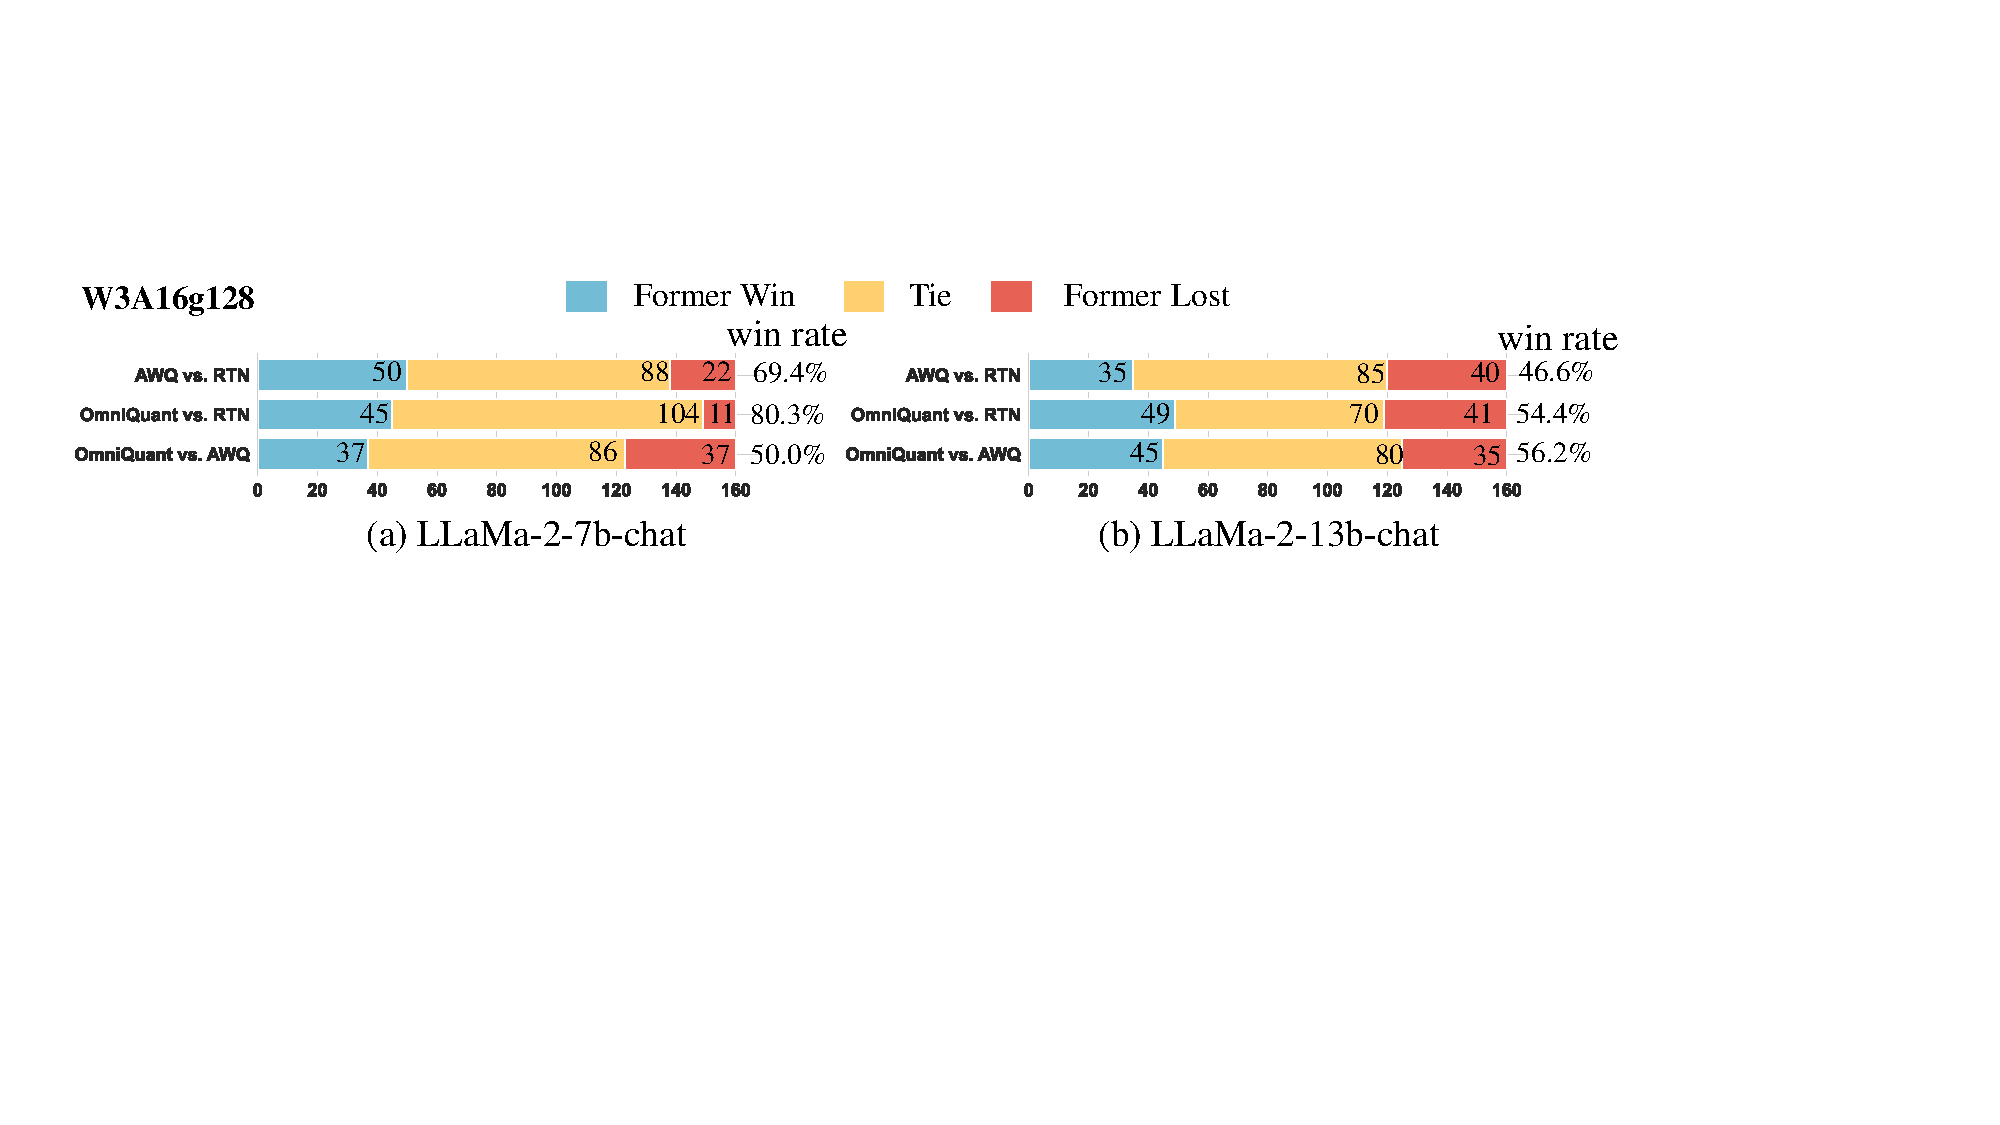
\includegraphics[width=0.9\textwidth]{gpt4_evaluation.pdf}
    \vspace{-1em}
    \caption{Comparing W3A16g128 quantization among RTN, AWQ~\citep{awq}, and OmniQuant under Vicuna-Bench~\citep{vicuna}. Win rates are calculated without considering tie samples. A higher win rate indicates the better performance of the former of \emph{vs.} pairs.}
    \label{fig:gpt4_evaluation}
    \vspace{-1em}
\end{figure}




\subsection{Acceleration on Real Device}\label{sec:deployment}
% MLC-LLM\footnote{https://github.com/mlc-ai/mlc-llm} offers a universal deployment solution suitable for various language models across a wide range of hardware backends, encompassing iPhones, Android phones, and GPUs from NVIDIA, AMD, and Intel. Notably, MLC-LLM emerges as the optimal solution for deploying quantized models on CUDA.
% %
% A notable advantage of OmniQuant is that it does not introduce additional operations for quantized models. Consequently, MLC-LLM can natively execute the quantized models developed using OmniQuant.
% %
% Table\,\ref{tab:speed} delineates the memory requirements and inference speeds of the LLaMA family on a single NVIDIA A100-80G. `Weights Memory (WM)' characterizes the storage utilized by quantized weights, while `Running Memory (RM)' signifies the memory needed for practical inference. The latter is notably greater due to the need to retain certain intermediate activations. Our evaluation metric for inference speed is the generation of 512 tokens from scratch.
% %
% It is evident that quantized models drastically curtail memory usage compared to the full-precision (16-bit) counterparts. For example, models with W4A16g128 and W2A16g128 quantization display nearly a $2\times$ enhancement in inference speed. However, MLC-LLM's support for INT3/INT2 is currently suboptimal, particularly for INT3. Enhancements to INT3/INT2 quantization speed are in our future roadmap.
% %
% Additionally, we only explore the deployment of weight-only quantization in this study due to that W4A4 and W6A6 quantization methods lack out-of-the-box hardware support.


MLC-LLM\footnote{https://github.com/mlc-ai/mlc-llm} provides a versatile deployment solution for diverse language models across various hardwares. It particularly excels in deploying quantized models on CUDA.
%
One of OmniQuant's strengths lies in its ability to avoid extra operations for quantized models, allowing MLC-LLM to seamlessly run models created with OmniQuant.
%
Table,\ref{tab:speed} shows memory requirements and inference speeds of the LLaMA family on an NVIDIA A100-80G. 'Weights Memory (WM)' represents quantized weight storage, and 'Running Memory (RM)' indicates the memory for inference, with the latter being higher due to certain retained activations. Inference speed is gauged by generating 512 tokens.
%
It is evident that quantized models significantly reduce memory usage compared to 16-bit full-precision models. For instance, models with W4A16g128 and W2A16g128 quantization almost double the inference speed. However, MLC-LLM's support for INT3/INT2 is currently suboptimal, particularly for INT3. Enhancements to INT3/INT2 quantization speed are in our future roadmap.
%
Additionally, we only explore the deployment of weight-only quantization in this study due to that W4A4 and W6A6 quantization methods lack out-of-the-box hardware support.


\begin{table}[!t]
    \centering
    % \setstretch{0.8}
    \renewcommand{\arraystretch}{0.7}
    \setlength{\tabcolsep}{1pt}
    \caption{Deployment of weight-only quantization through MLC-LLM. We report the memory size of quantized weights (denoted as `WM') and the running memory (denoted as `RM') and speed in NVIDIA A100-80G. }
    \begin{tabular}{ccccccccccccc}
    \hline
    \textbf{LLaMA} & \multicolumn{3}{c}{\textbf{7B}} & \multicolumn{3}{c}{\textbf{13B}} & \multicolumn{3}{c}{\textbf{30B}} & \multicolumn{3}{c}{\textbf{65B}} \\
    \cmidrule(l{2pt}r{2pt}){2-4}
    \cmidrule(l{2pt}r{2pt}){5-7}
    \cmidrule(l{2pt}r{2pt}){8-10}
    \cmidrule(l{2pt}r{2pt}){11-13}
     & WM & RM &  token/s & WM & RM &  token/s  & WM & RM &  token/s  & WM & RM &  token/s \\
     \hline
    FP & 12.6G &	14.4G&	69.2&	24.3G &	27.1G &	52.5 &	60.6G&	66.1G	&23.9	&OOM&	-&	-\\
    W4A16g128 & 3.8G&	5.7G&	134.2&	7.0G&	10.0G&	91.3&	16.7G&	21.7G&	43.6&	33.0G&	41.0G&	24.3\\
    W3A16g128 &3.2G	&5.1G&	83.4&	5.8G&	8.7G&	57.6&	13.7G&	18.7G&	29.0&	27.0G&	35.1G&	15.2\\
    W2A16g128& 2.2G&	4.1G&	83.9&	4.0G&	7.5G&	92.6&	9.2G&	14.1G&	36.7&	18.0G&	25.6G&	24.8\\
    \hline
    \end{tabular}
    \vspace{-1.5em}
    \label{tab:speed}
\end{table}






% \subsection{Ablation Studies} 

% In this section, we evaluate the performance contributions of LWC and LET. Further ablation studies, encompassing the design of LET, training duration, and calibration datasets, can be found in Appendix Sec~\ref{sec:more_ablation}.
% %
% As demonstrated in Table,\ref{tab:ablation}, the baseline model activates both LWC and LET, labeled as 'LWC+LET'. Subsequently, the unique contributions of LWC and LET to overall performance are assessed by sequentially deactivating each.
% %
% Unsurprisingly, each component has a positive impact on final performance. However, LET emerges as particularly critical in weight-activation quantization. When deactivated for W4A4, the model experiences a dramatic surge in perplexity to $e3$. This significant increase is attributed to the challenge posed by outliers in activation quantization, a problem effectively ameliorated by the implementation of LET.
% %
% In the case of weight-only quantization, the implementation of LET substantially improves the performance of OPT, while only providing marginal improvement for LLaMA. This variation can be attributed to the minimal presence of outliers in LLaMA's weights. For instance, during naive W3A16 quantization (-LWC-LET), LLaMA's performance reaches a perplexity of 10.68, whereas OPT's perplexity dramatically escalates to $4.6e3$.
% %
% Hence, for weight-only quantization, LET is deactivated for LLaMA due to its negligible benefit.

% In this section, we assess the performance impacts of LWC and LET. Detailed ablation studies, including LET's design, training time, and calibration datasets, are provided in Appendix Sec~\ref{sec:more_ablation}.
% %
% Table~\ref{tab:ablation} reveals that the baseline model incorporates both LWC and LET, labeled as 'LWC+LET'. We further investigate their individual contributions by remove each component.
% %
% Both components positively influence performance, but LET proves essential for weight-activation quantization. Disabling it for W4A4 results in a sharp rise in perplexity to $e3$, primarily due to challenges with activation quantization outliers.
% %
% For weight-only quantization, LET significantly boosts OPT's performance but offers slight enhancement for LLaMA, explained by LLaMA's few weight outliers. For example, in naive W3A16 quantization (-LWC-LET), LLaMA reaches a perplexity of 10.68, while OPT's spikes to $4.6e3$.
% %
% Consequently, LET is turned off for LLaMA in weight-only quantization given its limited advantage for faster training.









\section{Conclusion}
% In this study, we introduce OmniQuant, an innovative method designed to propel both weight-only quantization and weight-activation quantization into low-bit formats. The foundational insight of OmniQuant involves freezing the original full-precision weights while introducing additional learnable parameters. Specifically, OmniQuant leverages learnable weight clipping and learnable equivalent transformation to render weight and activation more compatible with quantization. Despite integrating gradient updates, OmniQuant conserves training time and data efficiency on par with prevalent PTQ methods. It surpasses existing techniques in language generation and zero-shot tasks and is viable for application in instruction-tuned LLMs. Additionally, OmniQuant demonstrates hardware efficiency as all additional learnable parameters can be absorbed, ensuring its compatibility with existing kernels.

We present OmniQuant, a method advancing weight-only and weight-activation quantization to low-bit formats. OmniQuant's core principle is to retain original full-precision weights while adding learnable parameters. It uses learnable weight clipping and learnable equivalent transformation to optimize weight and activation for quantization. While incorporating gradient updates, OmniQuant maintains training efficiency comparable to existing PTQ methods. It outperforms current methods in language generation and zero-shot tasks and is suited for instruction-tuned LLMs. In addition, OmniQuant also ensures hardware compatibility as its added parameters can be absorbed.



\subsubsection*{Acknowledgments}
This paper is partially supported by the National Key R\&D Program of China  No.2022ZD0161000 and the General Research Fund of Hong Kong No.17200622. We thank Wentao Liu from SenseTime for his valuable insights and discussions regarding LLM deployment. We also acknowledge Siyuan Feng from Apache TVM for assisting in deploying our OmniQuant in the MLC LLM project.


\bibliography{iclr2024_conference}
\bibliographystyle{iclr2024_conference}

\appendix

\renewcommand{\thetable}{A\arabic{table}}
\renewcommand{\thefigure}{A\arabic{figure}}
\renewcommand{\theequation}{A\arabic{equation}}
\renewcommand{\thesection}{A\arabic{section}}

\setcounter{table}{0}
\setcounter{figure}{0}

In this appendix, we provide further details as follows:
\begin{itemize}
\item Sec.\ref{sec:algorithm}: Presents the pseudo code for our OmniQuant algorithm.
\item {Sec.\ref{sec:distinctions}: Summarizes the distinctions with existing equivalent transformation methods}.
\item Sec.\ref{sec:ablation-studies}: Details ablation studies, encompassing the efficacy of each component, design choices for the learnable equivalent transformation, training time, and calibration data, etc.
\item Sec.\ref{sec:training-time}: Provides the detailed training time for the LLaMA family.
\item Sec.\ref{sec:performance-analysis}: Explores the internal mechanisms of the proposed method.
\item Sec.\ref{sec:comparisons-with-clipping}: Compares the proposed LWC with other clipping-based quantization approaches.
\item Sec.\ref{sec:full-results}: Showcases the complete results for OPT, LLaMA-1, LLaMA-2, and Falcon models.
\end{itemize}

\section{Overall algorithm}\label{sec:algorithm}
The comprehensive training algorithm of OmniQuant is illustrated in Algorithm\,\ref{alg:omniquant}.
%
We employ a block-wise calibration strategy comprising three steps: initialization of learnable parameters (Lines 4-5), training these learnable parameters (Lines 6-15), transforming the model with learned parameters, and then quantization(Lines 16-18).
%
The OmniQuant algorithm finds the optimal transformation to enhance the quantization compatibility of the LLM model. Additionally, due to the elegant design, OmniQuant can achieve rapid convergence using a small calibration dataset.

\begin{algorithm}[!ht]
\caption{Overall algorithm of OmniQuant.}\label{alg:omniquant}
\textbf{Input}: calibration dataset $\mathbf{X}$, pre-trained LLM model $\mathcal{M}$  \\
\textbf{Output}: quantized model.
\begin{algorithmic}[1]
\State $\mathbf{X}_{fp}$ = $\mathbf{X}_{q}$ = $\mathbf{X}$  \Comment{init inputs of full-precision and quantized models.}
\For {$\mathcal{B}_i$ in $\mathcal{M}$}:  \Comment{block-wise calibration}
\State $\mathbf{X}_{fp} = \mathcal{B}_i(\mathbf{X}_{fp})$ \Comment{update the input of full-precision model}
\State init learnable weight clipping parameters $\Theta_1$
\State init learnable equivalent transformation $\Theta_2$
\For {k in epochs}:
\For{($\mathbf{x}_{q}$,$\mathbf{x}_{fp}$) in ($\mathbf{X}_{q}$,$\mathbf{X}_{fp} )$}
\State $\mathcal{B}_i^{'}$ = LET($\mathcal{B}_i$,$\Theta_2$) \Comment{With Eq.(\ref{eq:original_linear}),Eq.(\ref{eq:LET-attn})}
\State $\mathcal{B}_i^{'}$ = Quantization\_with\_LWC($\mathcal{B}_i^{'}$,$\Theta_1$)\Comment{With Eq.(\ref{eq:LWC})}
\State $\mathbf{x}_{q}^{'}$ = $\mathcal{B}_i^{'}(\mathbf{x}_{q})$
\State loss = $\lvert\lvert \mathbf{x}_{fp} -\mathbf{x}_{q}^{'} \rvert\rvert^{2}$ \Comment{With Eq.(\ref{eq:objective})}
\State loss.backward()
\State update $\Theta_1$ and $\Theta_2$ through gradient
\EndFor
\EndFor
\State $\mathcal{B}_i$ = LET($\mathcal{B}_i$,$\Theta_2$) 
\State $\mathcal{B}_i$ = Quantization\_with\_LWC($\mathcal{B}_i$,$\Theta_1$) \Comment{obtain the quantized block}
\State $\mathbf{X}_q$ = $\mathcal{B}_i(\mathbf{X}_q)$ \Comment{update the input of quantized model}
\EndFor
\State \textbf{return} quantized model $\mathcal{M}$
\end{algorithmic}
\end{algorithm}


\begin{table}[!ht]
    \centering
    \caption{\textbf{Distinction of existing equivalent transformation methods.}}
    \setlength{\tabcolsep}{1pt}
    \resizebox{\linewidth}{!}{\color{black}
    \begin{tabular}{ccccc}
    \hline
    Method & ET operation & ET position & ET parameters & application \\
    \hline
    SmoothQuant & scaling & linear layer & pre-defining & weight-activation quantization \\
    \hline
    AWQ & scaling & linear layer & grid searching & weight-only quantization \\
    \hline
    \multirow{2}{*}{OP+} & scaling  & \multirow{2}{*}{linear layer}  & grid searching for scaling  & \multirow{2}{*}{weight-activation quantization}\\
    & \& shifting & & and pre-defining for shifting & \\
    \hline
    \multirow{2}{*}{OmniQuant}  & scaling & linear layer  & \multirow{2}{*}{\textbf{gradient-based optimization}}  & \textbf{weight-only quantization}  \\
    &  \& shifting & \textbf{\& attention} & & \& \textbf{weight-activation quantization} \\
    \hline
    \end{tabular}
    \label{tab:distinction}
    }
\end{table}

\color{black}
\section{Distinction of existing equivalent transformation methods}\label{sec:distinctions}
Equivalent transformation is popular in the quantization of large language models. In this section, we summarize the distinction of proposed OmniQuant with existing equivalent transformation works, including SmoothQuant~\citep{smoothquant}, AWQ~\cite{awq}, Outlier Supression (OP+)+~\cite{outlier-plus}. As shown in Table~\ref{tab:distinction}:
\begin{itemize}
    \item For the equivalent transformation operation, both SmoothQuant and AWQ only consider channel-wise scaling operation, while OP+ and OmniQuant consider both channel-wise scaling and shifting operation.
    \item For the execution position, previous methods only carry equivalent transformation on linear layers (Eq.(\ref{eq:LET-linear})), while OmniQuant also considers the matrix multiplication within attention  (Eq.(\ref{eq:LET-attn})). This point enlarges the solution space of equivalent transformation and facilitates the quantization of $\mathbf{Q}$ and $\mathbf{K}$.
    \item For the manners to obtain parameters of equivalent transformation, SmoothQuant leverage pre-defined migration strength. Then, AWQ and OP+ introduce grid searching based on some heuristic proxy. However, OmniQuant optimized all equivalent transformation parameters through end-to-end gradient descent, which significantly improve the performance.
    \item For the application scenario, previous methods are designed for weight-only quantization or weight-activation quantization. However, because of the elegant design and cooperation of the proposed LWC and LET, OmniQuant can achieve excel in both weight-only quantization and weight-activation quantization.
\end{itemize}
\color{black}


\section{Ablation studies}\label{sec:ablation-studies}

\begin{table}[!ht]
    \centering
    \caption{\textbf{Effect of combination of equivalent transformation and weight clipping}. We report the average perplexity of WikiText2 and C4, and the average accuracy on 6 zero-shot tasks like Table 2.}
    \begin{tabular}{lcc}
    \hline
    \textbf{LLaMa-7B W4A4} & \textbf{Average PPL $\downarrow$} & \textbf{Average Acc. $\uparrow$} \\
    \hline
    SmoothQuant & 28.78 & 38.41 \\
    LET & 16.97 & 48.83\\
    LET + grid-searched WC & 15.82 & 49.59 \\
    SmoothQuant + LWC & 15.80 & 50.15 \\
    \textbf{LET + LWC} & \textbf{12.87} & \textbf{52.65} \\
    \hline
    \end{tabular}
    \label{tab:ablation_combination}
\end{table}
\color{black}
\textbf{Combination of equivalent transformation and weight clipping.} The synergy between LET and LWC is achieved through a sophisticated differentiable framework as demonstrated in Algorithm~\ref{alg:omniquant}, not a simple additive combination. LET performs activation-to-weight migration, and LWC further facilitates the quantization of weights, resulting in a seamless integration of the two techniques. In Table~\ref{tab:ablation_combination}, we also test other combination variants, including replacing LET with SmoothQuant or replacing LWC with grid-searched weight clipping. The results show that training LET and LWC simultaneously achieves the best performance.


\color{black}


\begin{table}[!ht]
    \centering
    \caption{\textbf{Efficacy of each component.} WikiText2 perplexity1 is reported in this table. `-' indicats remove the corresponding module from the overall proposed methods.}
    \begin{tabular}{llcccc}
    \hline
    \multicolumn{2}{c}{\textbf{PPL}$\downarrow$} & \multicolumn{2}{c}{\textbf{LLaMA-13B}} & 
    \multicolumn{2}{c}{\textbf{OPT-13B}} \\
    \cmidrule(l{2pt}r{2pt}){3-4}
    \cmidrule(l{2pt}r{2pt}){5-6} 
    \multicolumn{2}{c}{\textbf{Method}} & W4A4 & W3A16 & W4A4 & W3A16  \\
    \hline
     & \textbf{LWC+LET} & \textbf{10.87} & \textbf{5.65} & \textbf{11.65} & \textbf{10.87} \\
     \hline
    \multirow{3}{*}{\shortstack{components}}  & -LWC & 20.75 & 7.65 & 15.23 & 12.98 \\
    & -LET & 5.4e3 & 5.68 & 7.8e3 & 11.29 \\
    & -LWC-LET & 1.8e3 & 10.68 & 7.8e5 & 4.6e3 \\
    \hline
    \end{tabular}
    \label{tab:ablation}
\end{table}



\textbf{Efficacy of each component.} Table~\ref{tab:ablation} reveals that the baseline model incorporates both LWC and LET, labeled as 'LWC+LET'. We further investigate their contributions by removing each component.
%
Both components positively influence performance, but LET proves essential for weight-activation quantization. Disabling it for W4A4 results in a marked increase in perplexity to $e3$, mainly due to challenges with activation quantization outliers.
%
For weight-only quantization, LET significantly boosts OPT's performance but offers a slight enhancement for LLaMA, explained by LLaMA's few weight outliers. For example, in naive W3A16 quantization (-LWC-LET), LLaMA reaches a perplexity of 10.68, while OPT's spikes to $4.6e3$.
%
Consequently, LET is turned off for LLaMA in weight-only quantization given its limited advantage for faster training.

\begin{table}[!ht]
    \centering
    \caption{\textbf{Design choices of learnable equivalent transformation.} WikiText2 perplexity1 is reported in this table. }
    \begin{tabular}{llcccc}
    \hline
    \multicolumn{2}{c}{\textbf{PPL}$\downarrow$} & \multicolumn{2}{c}{\textbf{LLaMA-13B}} & 
    \multicolumn{2}{c}{\textbf{OPT-13B}} \\
    \cmidrule(l{2pt}r{2pt}){3-4}
    \cmidrule(l{2pt}r{2pt}){5-6} 
    \multicolumn{2}{c}{\textbf{Method}} & W4A4 & W3A16 & W4A4 & W3A16  \\
    \hline
     & \textbf{LWC+LET} & \textbf{10.87} & \textbf{5.65} & \textbf{11.65} & \textbf{10.87} \\
     \hline
    \multirow{2}{*}{\shortstack{LET}} & -shifting & 11.47 & 5.65 & 13.64 & 10.87 \\
    & -attention & 11.34 & 5.65 & 11.79 & 10.87\\
    \hline
    \end{tabular}
    \label{tab:ablation_let}
\end{table}

\textbf{Design choices of learnable equivalent transformation.} 
In comparison to the equivalent transformation incorporated in SmoothQuant~(\cite{smoothquant}), our approach additionally implements channel-wise shifting and attention transformation. The effects of these innovations are evaluated in Table~\ref{tab:ablation_let}. We can observe that both modifications enhance the performance of weight-activation quantization. However, the incremental benefit of the equivalent transformation in the attention operation is comparatively minor. This discrepancy is primarily due to the majority of outliers existing in the output of the normalization layer while being less prevalent in the $Q/K/V$ matrix.

\begin{table}[!ht]
    \centering
    \caption{\textcolor{black}{\textbf{Impact of LET on each position.} `-' indicates removing corresponding LET. We respectively remove the LET from each layer, and reporting the average perplexity of WikiText2 and C4, and the average accuracy on 6 zero-shot tasks like Table 2.}}
    \color{black}
    \begin{tabular}{lcc}
    \hline
    \textbf{LLaMa-7B} & \textbf{Average PPL $\downarrow$} & \textbf{Average Acc. $\uparrow$} \\
    \hline
    \textbf{W4A4} & \textbf{12.87} & \textbf{52.65} \\
    -[ln1, (q\_proj, k\_proj, v\_proj)] & 19.87 & 46.79 \\
    -[v\_proj, out\_proj] & 13.03 & 51.68 \\
    -[Q,K] & 13.34 & 51.47 \\
    -[ln2, fc1] & 14.47 & 51.04 \\
    \hline
    \end{tabular}
    \label{tab:ablation_let_position}
\end{table}

\textcolor{black}{
\textbf{Impact of LET on each position.} We exclude the LET of the second linear layer due to the high sparsity of features after the non-linear layer leads to unstable gradients. Therefore, we have four LET pairs, represented as [ln1, (q\_proj, k\_proj, v\_proj)], [v\_proj, out\_proj], [Q, K], and [ln2, fc1].  As shown in Table~\ref{tab:ablation_let_position}, we can find that all four LETs can improve the performance, specially for the [ln1, (q\_proj, k\_proj, v\_proj)] pair. Such results also demonstrate that the activation outliers are more serious after layer normalization layers.
}


\begin{table}[!ht]
    \centering
    \caption{\textcolor{black}{\textbf{Impact of initialization of LET.} We report the average perplexity of WikiText2 and C4, and the average accuracy on 6 zero-shot tasks like Table 2.}}
    \color{black}
    \begin{tabular}{lcc}
    \hline
    \textbf{LLaMa-7B} & \textbf{Average PPL $\downarrow$} & \textbf{Average Acc. $\uparrow$} \\
    \hline
    \textbf{W4A4} & \textbf{12.87} & \textbf{52.65} \\
    initialize scaling as 1 & 13.64 & 51.37 \\
    initialize shifting as 0 & 12.95 & 52.22 \\
    \hline
    \end{tabular}
    \label{tab:ablation_initialization}
\end{table}

\textcolor{black}{
\textbf{Impact of initialization of LET.} We initialize the channel-wise scaling factor with SmoothQuant~\cite{smoothquant}, and initialize the channel-wise shifting with Outlier Suppression+~\cite{outlier-plus}. To validate the impact of careful initialization, we try to initial scaling as 1 and initial shifting as 0. As shown in Table~\ref{tab:ablation_initialization}, we can find that careful initialization of scaling and shifting can improve the final performance. Specifically, scaling initialization is more important than shifting, since scaling plays the main role in alleviating outliers.
}

\begin{table}[!ht]
    \centering
    \caption{\textcolor{black}{\textbf{Impact of Softmax quantization.} We report the average perplexity of WikiText2 and C4, and the average accuracy on 6 zero-shot tasks like Table 2.}}
    \color{black}
    \begin{tabular}{lcc}
    \hline
    \textbf{LLaMa-7B} & \textbf{Average PPL $\downarrow$} & \textbf{Average Acc. $\uparrow$} \\
    \hline
    \textbf{W4A4 + Softmax 16bit} & \textbf{12.87} & \textbf{52.65} \\
    W4A4 + Softmax 8bit & 12.91 & 51.93 \\
    W4A4 + Softmax 6bit & 13.20 & 51.70 \\
    W4A4 + Softmax 4bit & 18.80 & 48.52 \\
    \hline
    \end{tabular}
    \label{tab:ablation_softmax}
\end{table}

\color{black}
\textbf{Impact of Softmax quantization.}  The output of SoftMax has a long-tailed distribution, making it unsuitable for uniform quantization. We carry out experiments to quantize the Softmax output into different bit numbers. As shown in the following table, we can find that quantizing the output of softmax into 8-bit and 6-bit bring acceptable performance degeneration, which demonstrates that block-wise calibration can compensate for the loss of 8-bit and 6-bit Softmax quantization. However,  4-bit Softmax quantization brings significantly performance loss, which requires further exploration and additional trick such as log2 quantization in RepQViT~\citep{repqvit}. Note that we keep the output of SoftMax as 16-bit if no special instruction.
\color{black}

\begin{table}[!ht]
    \centering
    \caption{\textcolor{black}{\textbf{Impact of iterative training of LWC and LET.} We report the average perplexity of WikiText2 and C4, and the average accuracy on 6 zero-shot tasks like Table 2.}}
    \color{black}
    \begin{tabular}{lcc}
    \hline
    \textbf{LLaMa-7B W4A4} & \textbf{Average PPL $\downarrow$} & \textbf{Average Acc. $\uparrow$} \\
    \hline
    \textbf{simultaneously} & \textbf{12.87} & \textbf{52.65} \\
    each iteration & 13.56 & 50.91 \\
    each epoch & 13.51 & 52.06 \\
    each epoch + double training epochs 4bit & 12.80 & 52.50 \\
    \hline
    \end{tabular}
    \label{tab:ablation_iteration}
\end{table}

\color{black}
\textbf{Impact of iterative training.} In our approach, LWC and LET are trained simultaneously, and we have also explored an iterative training approach by iterations or epochs. The results, as presented in Table~\ref{tab:ablation_iteration}, clearly indicate that training LWC and LET simultaneously yields the best performance. This experiment demonstrates that the synergy between LET and LWC creates a progressive process, where both techniques reinforce each other rather than interfere. To further support this statement, we conducted an additional experiment (last row in Table~\ref{tab:ablation_iteration}), training LWC and LET iteratively with double training epochs. The results show that simultaneous training with 20 epochs achieves comparable performance to iterative training with 40 epochs. This demonstrates the effectiveness and efficiency of training LWC and LET simultaneously.
\color{black}

\begin{table}[!ht]
    \centering
    \caption{\textbf{Ablation of training time.} We train LLaMA-7B with different quantization configuration on 128 2048-tokens segments from WikiText2 over various epochs. `0' indicates only initialization without fine-tuning. Wikitext perplexity is reported in this table.}
    \begin{tabular}{cccccc}
    \hline
    Epochs & W4A16 & W3A16 & W2A16 & W6A6 & W4A4 \\
    \hline
    0 & 6.29 & 24.04 & 1.1e5 & 6.16 & 33.93 \\
    10  & 5.87 & 6.51 & 27.49 & 5.96 & 12.04 \\
    20  & 5.85 & 6.49 & 17.46 & 5.95 & 11.26 \\
    40  & 5.86 & 6.47 & 15.47 & 5.95 & 11.23 \\
    80  & - & - & 14.77 & - & - \\
    \hline
    \end{tabular}
    \label{tab:ablation_time}
\end{table}





\textbf{Training Time}
As illustrated in Table~\ref{tab:ablation_time}, LLaMA-7B was trained across various epochs to determine the optimal convergence time. Most quantization configurations converge within 20 epochs, with the exception of W2A16, which necessitates 80 epochs. Consequently, we establish a training epoch of 20 for all configurations, except for W2A16, for which we set it to 40 in consideration of the training time.


\begin{table}[!ht]
    \centering
    \caption{\textbf{Ablation of calibration dataset.}}
    \begin{tabular}{ccccc}
    \hline
    \multicolumn{1}{c}{LLaMA-7B/\textbf{PPL}$\downarrow$} & \multicolumn{2}{c}{\textbf{W3A16}} & 
    \multicolumn{2}{c}{\textbf{W4A4}} \\ 
    \cmidrule(l{2pt}r{2pt}){2-3}
    \cmidrule(l{2pt}r{2pt}){4-5} 
    Calibration Dataset &  WikiText2 & C4 & WikiText2 & C4  \\
    \hline
    WikiText2 &  6.47 & 8.19 & 11.23 & 14.61 \\
    C4 & 6.67 & 8.13 & 12.17 & 14.24 \\  
    Pile & 6.69 & 8.17 & 12.04 & 14.22 \\
    \hline
    Varience & 0.009 & 0.0006 & 0.17 & 0.03 \\
    \hline
    \end{tabular}
    \label{tab:ablation_data}
\end{table}

\begin{table}[!ht]
    \centering
    \caption{\textbf{Ablation of sample number of calibration dataset.}}
    \begin{tabular}{ccccc}
    \hline
    \multicolumn{1}{c}{LLaMA-7B/\textbf{PPL}$\downarrow$} & \multicolumn{2}{c}{\textbf{W3A16}} & 
    \multicolumn{2}{c}{\textbf{W4A4}} \\ 
    \cmidrule(l{2pt}r{2pt}){2-3}
    \cmidrule(l{2pt}r{2pt}){4-5} 
    Sample Number &  WikiText2 & C4 & WikiText2 & C4  \\
    \hline
    16 &  6.47 & \textbf{8.18} & 11.56 & 14.84 \\
    32 & 6.47 & 8.18 & 11.48 & 14.80 \\  
    64 & 6.48 & 8.19 & 11.40 & \textbf{14.57} \\
    128 & 6.47 & 8.19 & \textbf{11.23} & 14.61 \\
    256 & \textbf{6.46} & 8.19 & 11.41 & 14.90\\
    \hline
    \end{tabular}
    \label{tab:ablation_data_number}
\end{table}


\textbf{Calibration Data}
OmniQuant utilizes gradient optimization on constrained calibration datasets, sourced from WikiText2 and comprising 128 segments with 2048 tokens each. This prompts concerns about potential overfitting to the calibration dataset. To explore this, we evaluated the calibration dataset's influence using two other datasets: Pile~(\cite{pile}) and c4~(\cite{c4}).
%
As depicted in Table~\ref{tab:ablation_data}, the variance in perplexity across diverse calibration datasets is marginal, fluctuating between 0.0006 and 0.17.  This underscores OmniQuant's robustness concerning calibration set distribution.
%
Furthermore, the data efficiency of OmniQuant was gauged by modulating the number of training samples, as presented in Table~\ref{tab:ablation_data_number}. Remarkably, OmniQuant converges with as few as 16 samples. Our selection of 128 samples aligns with established practices in prior works~(\cite{gptq,awq}).

\begin{table}[!ht]
    \centering
    \caption{Omniquant runtime on LLaMA family. The time correspond to training 128 2048-tokes segment over 20 epochs and a batch size of 1 on a single NVIDIA A100-80G.}
    \begin{tabular}{lcccc}
    \hline
    LLaMA & 7B & 13B & 30B & 65B \\
    \hline
    weight-only & 1.1h & 2.2h & 4.5h & 8.9h \\ 
    weight-activation & 1.6h & 3.3h & 7.3h & 14.4h\\
    \hline 
    \end{tabular}
    \label{tab:time}
\end{table}

\section{Training Time}\label{sec:training-time}
As shown in Table\,\ref{tab:time}, we report the training time of the proposed OmniQuant within the LLaMA family. Note that for LLaMA, we only activate learnable weight clipping for weight-only quantization. Therefore, the training time for weight-only quantization is shorter relative to weight-activation quantization, given the fewer learnable parameters involved.  While our proposed method necessitates a training time that is approximately 5$\times$ greater than GPTQ, it remains markedly faster than QAT methods, which demand hundreds of GPU hours.


\begin{table}[!ht]
    \centering
    \caption{\textbf{$l_1$ distance between quantized model and full-precision model.} $\lvert\lvert \mathbf{W} - \mathbf{W_q} \rvert\rvert$ indicates the average $l_1$ distance between quantized weight and full-precision weight.  $\lvert\lvert \mathbf{X} - \mathbf{X}_{q} \rvert\rvert$ denotes the $l_1$ distance between the output of last transformer block.}
    \begin{tabular}{cccccc}
    \hline
    \multicolumn{1}{c}{\textbf{LLaMA-7B / $l_{1}$ $\downarrow$}} & \multicolumn{2}{c}{$\lvert\lvert \mathbf{W} - \mathbf{W_q} \rvert\rvert$} & \multicolumn{2}{c}{$\lvert\lvert \mathbf{X} - \mathbf{X}_{q}\rvert\rvert$}  \\
    \cmidrule(l{2pt}r{2pt}){2-3}
    \cmidrule(l{2pt}r{2pt}){4-5} 
     quantization & w/o LWC & w/ LWC & w/o LWC & w/ LWC  \\
     \hline
     W2A16g128 & 0.0089 & \textbf{0.0082} & 3.24 &\textbf{1.36}\\
    W2A16g64 & 0.0098 & \textbf{0.0086} & 3.51 &\textbf{1.44}\\
     W3A16 & 0.0062 & \textbf{0.0044} & 2.80 &\textbf{1.05}\\
     W3A16g128 & 0.0042 & \textbf{0.0040} & 1.37 &\textbf{0.79}\\
     W4A16 & 0.0028 & \textbf{0.0024} & 0.98 &\textbf{0.61} \\
     W4A16g128 & 0.0020 & \textbf{0.0019} & 0.68 &\textbf{0.47}\\
     \hline
    \end{tabular}
    \label{tab:l1_distance}
\end{table}


\begin{figure}[!ht]
    \centering
    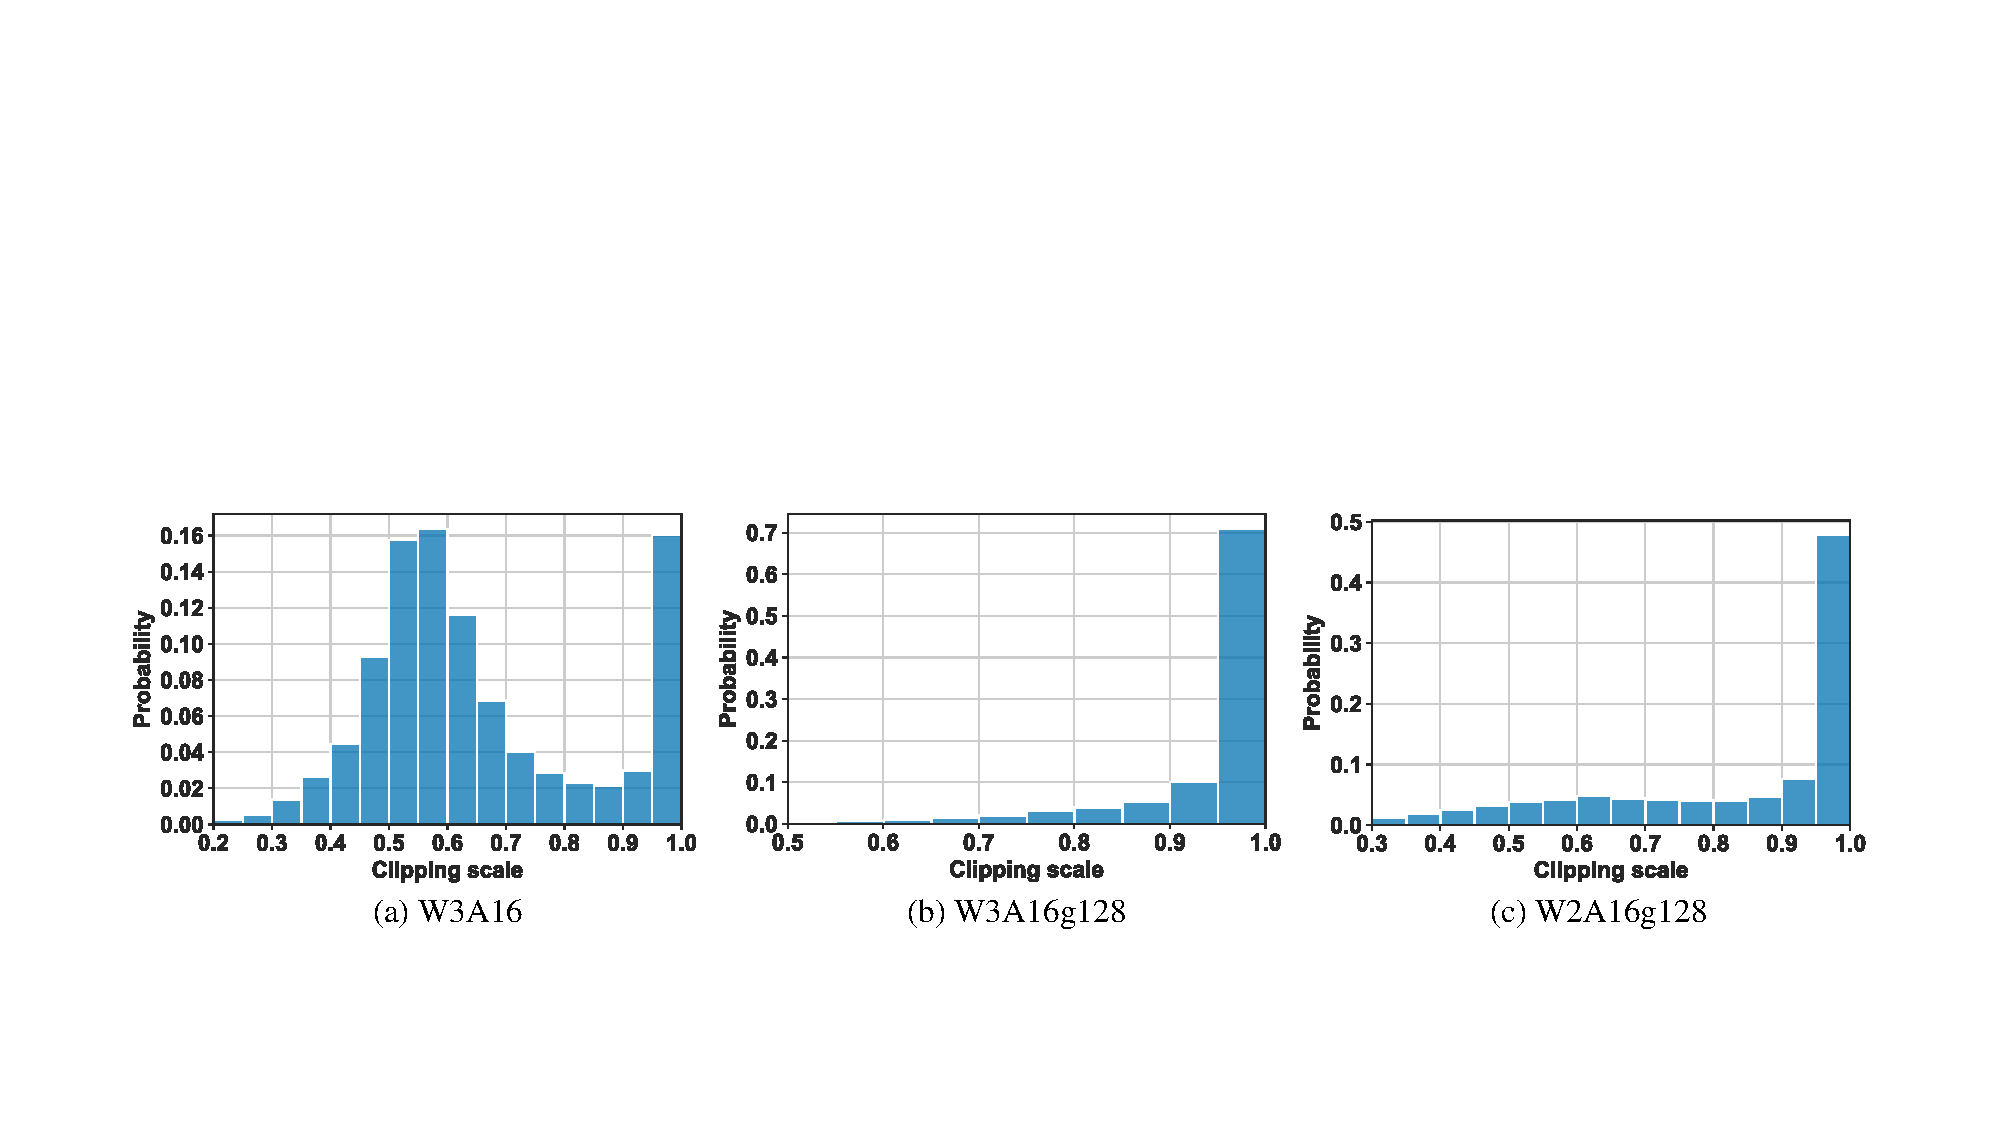
\includegraphics[width=\textwidth]{clipping_scale.pdf}
    \caption{Visualization of learned clipping scale in different quantization settings in LLaMA-7B.}
    \label{fig:clipping_scale}
\end{figure}


\section{Performance Analysis}\label{sec:performance-analysis}
In this section, we investigate the internal mechanism of learnable weight clipping and learnable equivalent transformation respectively. Further, we show that with OmniQuant, 3-bit and 4-bit achieve similar trade-off between model bits and perplexity.
%


\textbf{Learnable weight clipping.} 
In addition to perplexity and accuracy, the quality of a quantization method can intuitively be evaluated by calculating the distance between quantized models and their full-precision counterparts. This is demonstrated in Table \ref{tab:l1_distance}, where we detail the $l_1$ distance of weights and activations for LLaMA-7B's weight-only quantization.
%
We can observe that the proposed Learned Weight Clipping (LWC) substantially decreases the $l_1$ distance for both weights and activations. It's noteworthy that, in certain instances, the $l_1$ distance for quantized models without LWC is similar to that of those utilizing LWC. However, models incorporating LWC exhibit markedly lower activation $l_1$ distances.
%
This observation underpins the argument that LWC can effectively balance quantization precision between outlier and regular values.
%

Additionally, we illustrate the distribution of the learned clipping scale ($\gamma$ and $\beta$) as delineated in Eq. (\ref{eq:LWC}) in Figure \ref{fig:clipping_scale}.
%
It is apparent that LWC can learn different clippings for diverse quantization configurations. For instance, with per-channel weight quantization W3A16 as depicted in Figure \ref{fig:clipping_scale}(a), the learned clipping scale showcases a normal distribution. This suggests that approximately half of the outliers are being clipped.
%
In the case of group-wise quantization, the learned clipping scale exhibits a long-tailed distribution, implying that most quantized groups are associated with minimal clipping. Note that lower bits exhibit more pronounced clipping. For example, W2A16g128 possesses a 50\% clipping scale larger than 0.95, whereas, in W3A16g128, this percentage rises to 70\%.








\begin{figure}[!ht]
    \centering
    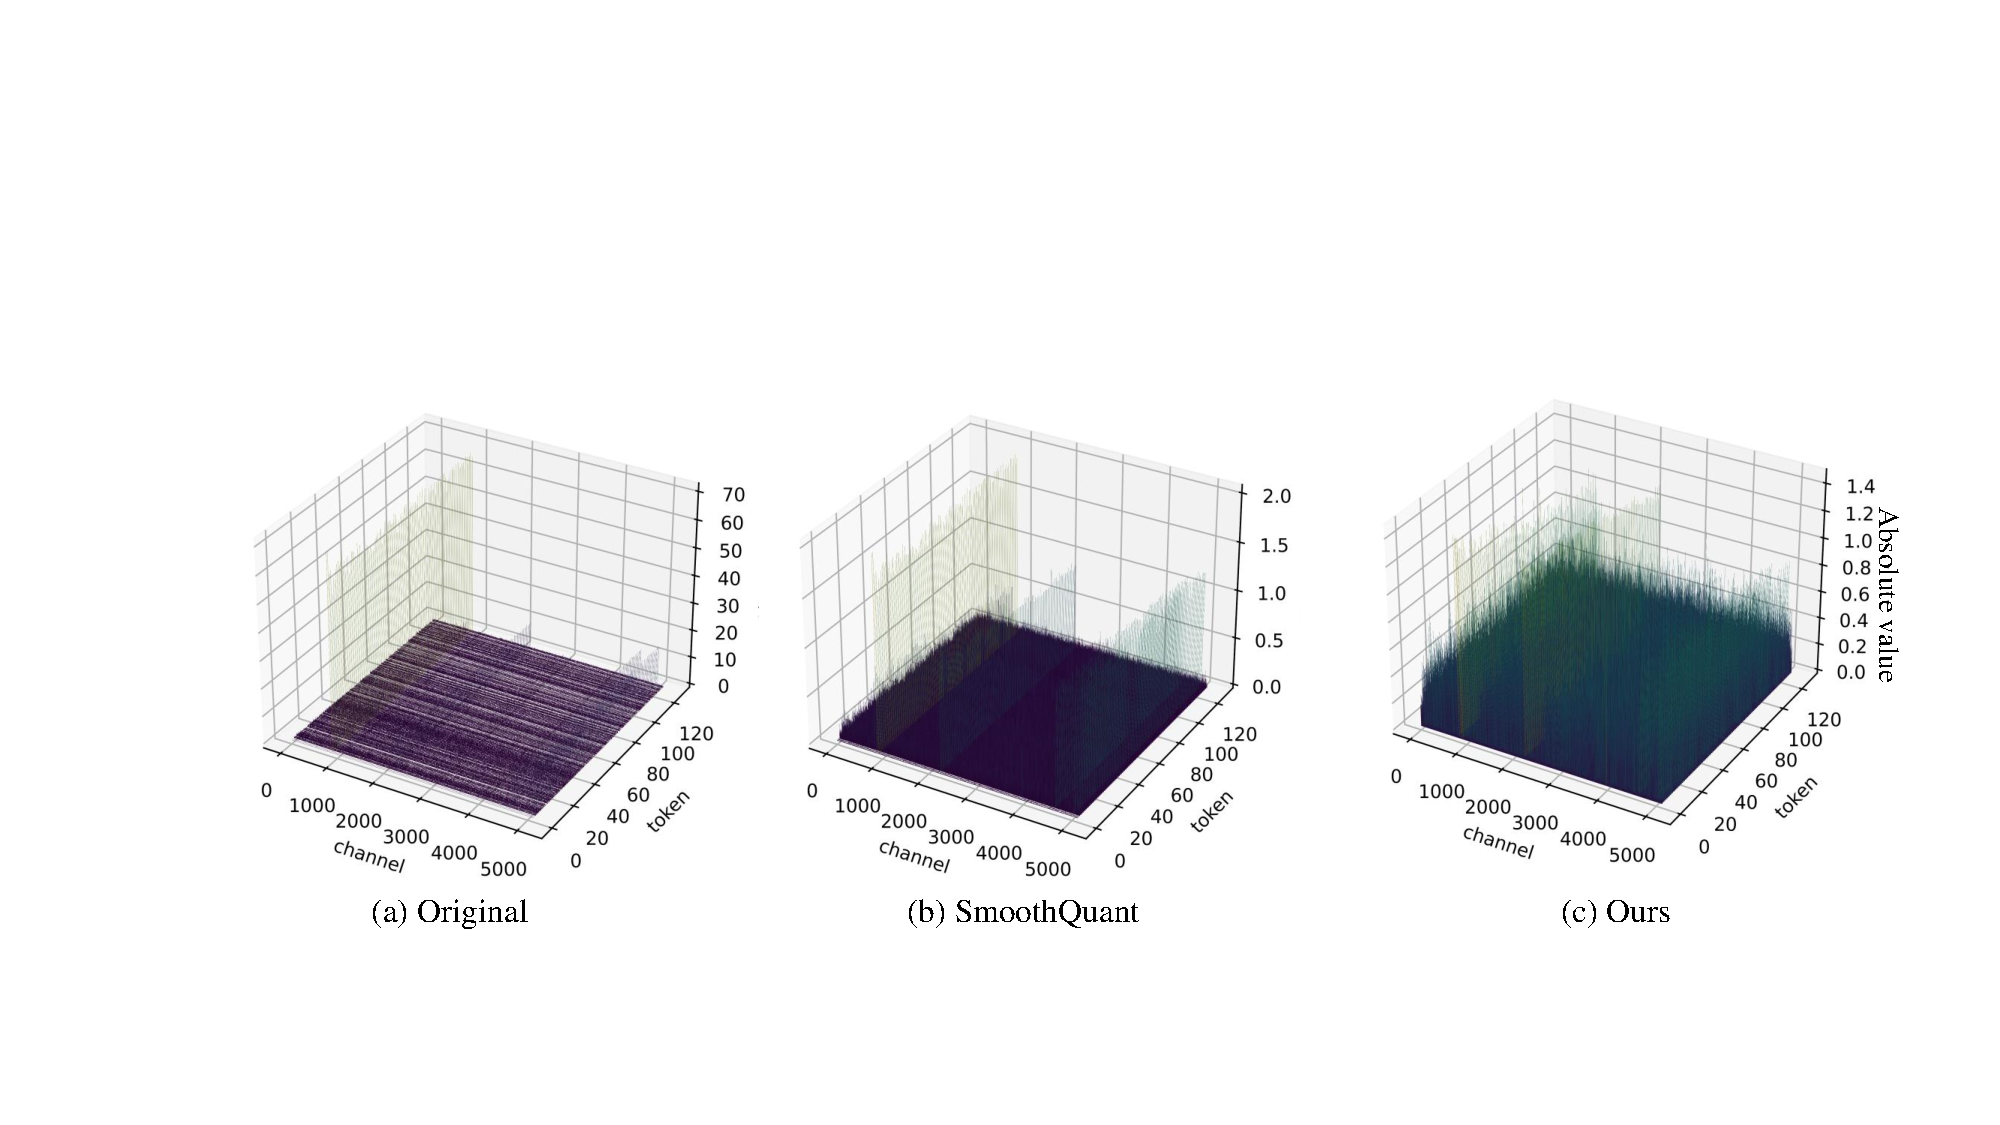
\includegraphics[width=0.9\textwidth]{activation.pdf}
    \caption{Visualization of activation of a linear layer in OPT-13B. (a) Original activation. (b) Activation after SmoothQuant. (c) Activation after proposed learnable equivalent transformation. Similar phenomena can be observed in different layer and different models.}
    \label{fig:activation}
\end{figure}



\textbf{Learnable equivalent transformation.}
Figure~\ref{fig:activation} provides visualizations of the intermediate activation in the linear layer. It is apparent that several outlier channels in the original activation (Figure~\ref{fig:activation}(a)) possess significantly larger magnitudes compared to the regular channels, thereby creating an incompatibility with activation quantization. 
%
Although SmoothQuant mitigates this issue to some degree, such as reducing the outlier magnitude from 70 to 2, Figure~\ref{fig:activation}(b) reveals that the magnitude of outlier channels still remains notably larger than that of other regular channels after SmoothQuant. This phenomenon can be attributed to SmoothQuant's heuristic approach in deriving channel-wise scaling, which inevitably makes it challenging to discover an optimal solution.
%
The impact of the proposed LET is depicted in Figure~\ref{fig:activation}(c). It is noteworthy that the magnitude disparity between the outlier and regular channels is markedly diminished. This homogenization of the activation distribution, facilitated by the LET, empowers OmniQuant to efficiently steer the weight-activation quantization towards a low-bit scheme.
%

\begin{figure}[!ht]
    \centering
    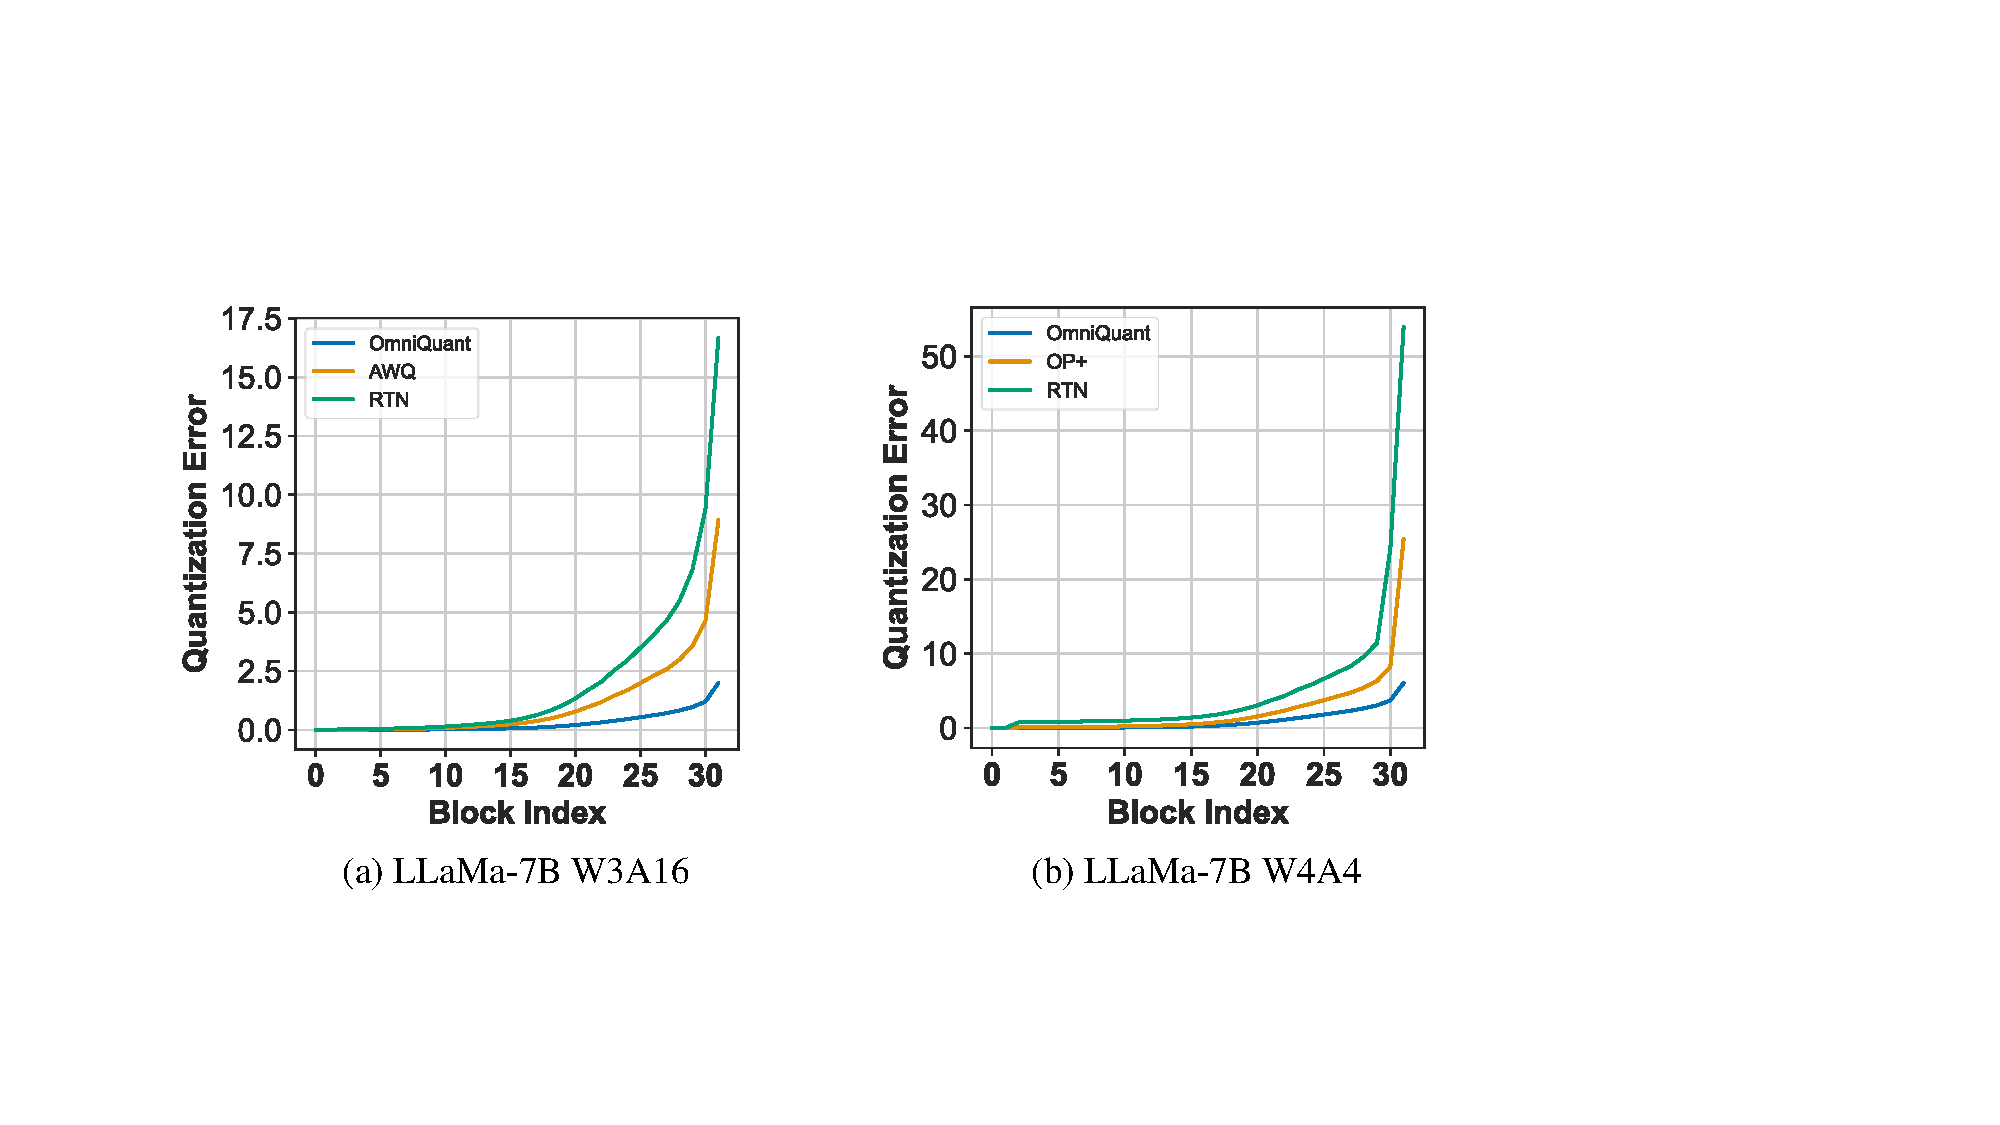
\includegraphics[width=0.75\textwidth]{quantization_error.pdf}
    \caption{\textcolor{black}{\textbf{Block-wise quantization error.} Grid-searched methods such as AWQ~\citep{awq} and Outlier Suppression +~\citep{outlier-plus} produce a more significant error than our gradient-based optimization method.}}
    \label{fig:quantization error}
\end{figure}

\textcolor{black}{
\textbf{Quantization error.}
OmniQuant is the first differentiable post-training quantization algorithm for large language models. To demonstrate the advantage of gradient-based optimization, we also compare the quantization error of each block in Figure~\ref{fig:quantization error}. We can find that OmniQuant significantly reduces the quantization loss compared with the grid-searching based method such as AWQ~\cite{awq} and Outlier Suppression +~\citep{outlier-plus}. 
}







\begin{figure}[!ht]
    \centering
    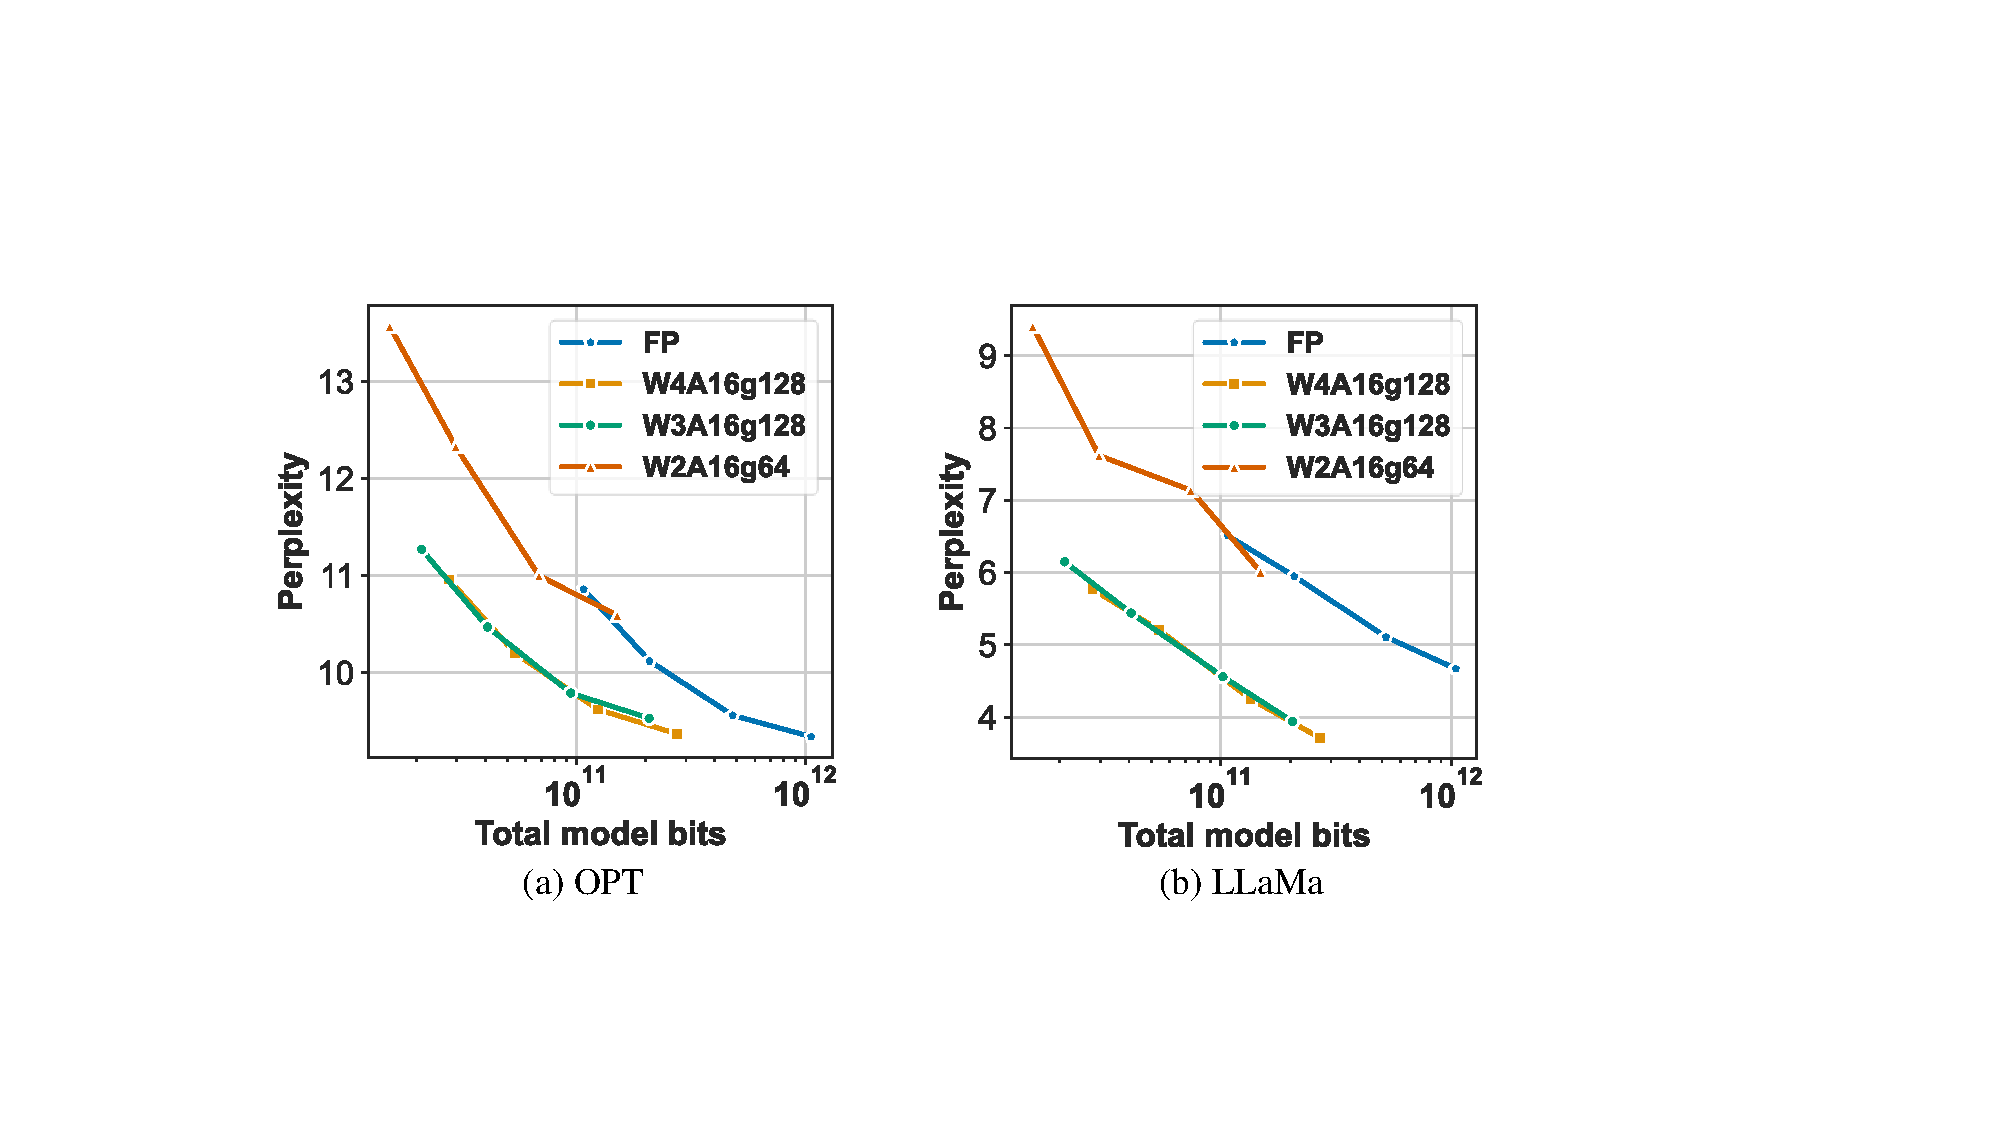
\includegraphics[width=0.8\textwidth]{trade_off.pdf}
    \caption{Bit-level scaling laws for perplexity.}
    \label{fig:trade-off}
\end{figure}

\textbf{Scaling laws.}
Quantization serves as a potent strategy to curtail the total model bits, thereby facilitating the deployment of LLMs on edge or consumer devices with restricted memory. However, the total model bits are contingent on both the number of parameters within the original model and the quantization bits. Therefore, given a model bits constraint, the challenge arises: how does one optimally determine the number of parameters for the full-precision model and the quantization bits?
%
Tim Dettmers~(\cite{scaline-law}) demonstrated that 4-bit quantization establishes a universally optimal balance between the total model bits and zero-shot accuracy. Nonetheless, in this study, as shown in Figure\,\ref{fig:trade-off},we would like to claim that OmniQuant can make 3-bit quantization achieve comparable performance like 4-bit quantization in the trade off between model bits and perplexity.


\begin{table}[!ht]
\centering
\caption{WikiText2 perplexity of clipping-based quantization methods. For fair comparison, we reproduce LSQ and PACT by replace LWC in our pipeline with them.}
\begin{tabular}{ccc}
\hline
\multicolumn{1}{c}{LLaMA-7B/\textbf{PPL}$\downarrow$} & \multicolumn{2}{c}{Perplexity} \\
Method &  W3A16 & W4A4   \\
\hline
FP &  \multicolumn{2}{c}{5.68}  \\
MinMax & 25.73 & 14.49 \\
PACT~(\cite{pact}) & 6.95 & 18.25\\
LSQ~(\cite{lsq}) & 6.63 & 15.03 \\
LWC (Ours) & \textbf{6.47} & \textbf{11.26} \\
\hline
\end{tabular}
\label{tab:clipping_method}
\end{table}


\begin{figure}[!ht]
    \centering
    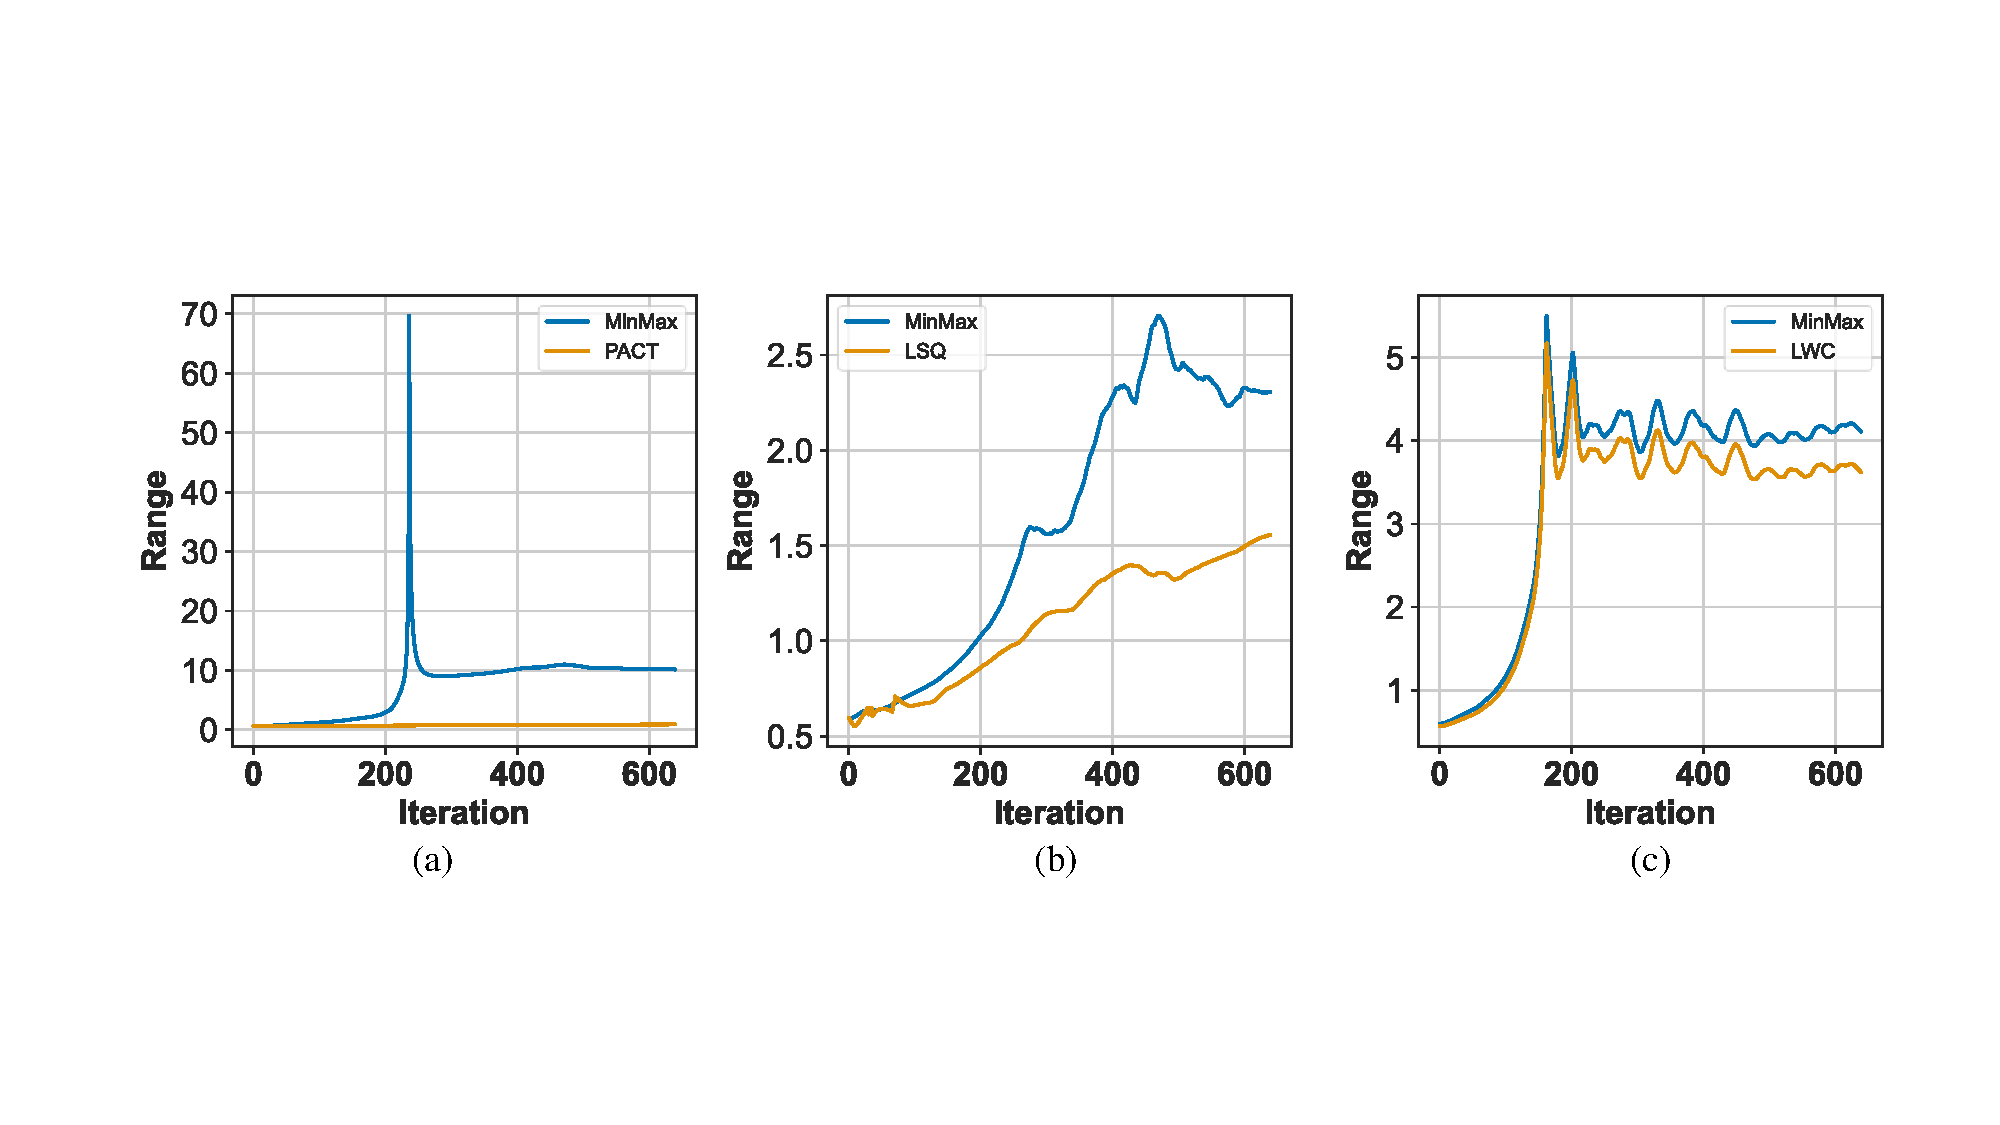
\includegraphics[width=0.9\linewidth]{weight_change.pdf}
    \caption{\textcolor{black}{\textbf{Weights range changing of different clipping-based methods during training.} We plot the changing of weights range (maximum minus minimum) of the 3049-th output channel of the q-proj linear layer in the first LLaMa-1-7B block with W4A4 quantization. MinMax is the baseline which indicate withoud clipping. Similar phenomena can also be observed in other channels and other layers.}}
    \label{fig:weight-change}
\end{figure}


\section{Comparisons with clipping-based methods}\label{sec:comparisons-with-clipping}
In this paper, we proposed a novel method, learnable weight clipping (LWC), designed to adaptively determine the weight clipping threshold. LWC sets the threshold by scaling the original minimum and maximum values to delineate the solution space. We compare LWC against existing clipping-based methods: PACT and LSQ. While PACT directly determines the clipping threshold, LSQ focuses on the direct derivation of the scaling factor and zero-point. Both PACT and LSQ were initially formulated as QAT methods, accounting for both weight and activation clipping. For an equitable comparison, our examination is restricted to weight clipping. We integrated PACT and LSQ into our optimization pipeline in lieu of LWC.
%
Table~\ref{tab:clipping_method} illustrates that while PACT and LSQ enhance the performance of weight-only quantization compared to MinMax quantization, their efficacy diminishes in the weight-activation quantization setting. This decline can be attributed to the proposed LET during activation quantization, which alters the weight distribution in each training iteration, undermining the convergence of both LSQ and PACT. In contrast, LWC defines relative scaling values instead of absolute metrics, making it proficient in handling changes in weight distribution. 
%
\textcolor{black}{For example, Figure~\ref{fig:weight-change} shows that LWC can catch the dramatically changing of weights while PACT and LSQ failed.}

%

\begin{table}[!ht]
    \centering
    \caption{\textcolor{black}{\textbf{Comparisons with SpQR and SqueezeLLM.}}}
\color{black}
\begin{tabular}{lcccc}
 % \multicolumn{4}{c}{LLAMA}
  % \multicolumn{2}{l}{\bf{LLaMa-1}}  & \multicolumn{3}{c}{}\\
 \toprule
 \bf{Size} & \bf{Method} & \bf{Avg bits} & \bf{Wiki2} & \bf{C4} \\
 \midrule
 % \midrule
 \multirow{8}{*}{LLaMa-1-7B} & -- & 16.00 & 5.68 & 7.08 \\
 & SpQR & 3.94 & 5.87 & 7.28\\
 & SqueezeLLM & 4.07 & 5.79 & 7.20 \\
 & SqueezeLLM & 4.27 & \textbf{5.77} & \textbf{7.18} \\
 & OmniQuant & 4.16 & \textbf{5.77} & 7.21 \\
 \cmidrule{2-5}
 & SqueezeLLM & 3.05 & 6.20 & 7.67 \\
 & SqueezeLLM & 3.24 & \textbf{6.13} & \textbf{7.56} \\
 & OmniQuant & 3.15 & 6.15 & 7.75 \\
 \midrule
 \multirow{8}{*}{LLaMa-1-13B} & -- & 16.00 & 5.09 & 6.61 \\
 & SpQR & 3.96 & 5.22 & 6.72 \\
 & SqueezeLLM & 4.07 & \textbf{5.17} & 6.69 \\
 & SqueezeLLM & 4.26 & \textbf{5.17} & \textbf{6.68} \\
 & OmniQuant & 4.16 & \textbf{5.17} & 6.69 \\
 \cmidrule{2-5}
 & SqueezeLLM & 3.04 & 5.51 & 7.01 \\
 & SqueezeLLM & 3.24 & 5.45 & \textbf{6.92} \\
 & OmniQuant & 3.15 & \textbf{5.44} & 7.05 \\
 \hline
 \multirow{8}{*}{LLaMa-1-30B} & -- & 16.00 & 4.10 & 5.98 \\
 & SpQR & 3.89 & 4.25 & 6.08 \\
 & SqueezeLLM & 4.06 & 4.20 & 6.05 \\
 & SqueezeLLM & 4.25 & \textbf{4.18} & \textbf{6.04} \\
 & OmniQuant & 4.16 & 4.19 & 6.06 \\
 \cmidrule{2-5}
 & SqueezeLLM & 3.04 & 4.56 & 6.31 \\
 & SqueezeLLM & 3.24 & \textbf{4.44} & \textbf{6.23} \\
 & OmniQuant & 3.15 & 4.56 & 6.37 \\
 \bottomrule
 \end{tabular}
    \label{tab:comparisons-with-mix}
\end{table}

\color{black}
\section{Comparisons with other weight-only quantization methods}\label{sec:comparisons-with-mix}
OmniQuant is an asymmetrically uniform quantization method. In the main paper, we compare with the same type of quantization methods, such as AWQ and GPTQ. Recently, there are also some other methods exploring for other quantization format. For example, SpQR~\citep{spqr} and SqueezeLLM~\citep{squeezellm} employ mixed-precision quantization to safeguard vital weights. Furthermore, SqueezeLLM also introduces non-uniform quantization to allocate more bits to sensitive weights. As shown in Table~\ref{tab:comparisons-with-mix}, we can find that OmniQuant can achieve comparable performance to SpQR and SqueezeLLM. While OmniQuant performs slightly worse than SqueezeLLM, our focus on uniform (INT) quantization provides simplicity and flexibility, supporting both weight-only quantization and weight-activation quantization. In contrast, SpQR and SqueezeLLM only support weight-only quantization. We believe this distinction adds valuable context to the comparison.
\color{black}







\section{Full Results}\label{sec:full-results}



In this section, we provide a comprehensive presentation of our results across various datasets to complement the main paper. Specifically, the results include:
\begin{itemize}
    % \item WikiText2 perplexity with weight-only quantization in the LLaMA families (Table \ref{tab:llama_weight_only_wiki}).
    \item The perform overview (Figure \ref{fig:performance_overview}).
    \item Experiments results on extreme large model Falcon-180B (Table \ref{tab:falcon-180b}).
    \item \textcolor{black}{MMLU results on LLaMa-1-7B (Table \ref{tab:mmlu})}.
    \item \textcolor{black}{Asymmetric bits quantization, including W4A8 on LLaMa-1-7B, W4A6, and W8A4. (Table \ref{tab: asymmetric_bits})}.
    \item C4 perplexity with weight-only quantization in the LLaMA families (Table \ref{tab:llama_weight_only_c4}).
    \item PTB perplexity with weight-only quantization in OPT families (Table \ref{tab:opt_weight_only_ptb}).
    \item C4 perplexity with weight-only quantization in OPT families (Table \ref{tab:opt_weight_only_c4}).
    \item WikiText2 perplexity for weight-activation quantization in the LLaMA families (Table \ref{tab:llama_weight_activation_wiki}).
    \item C4 perplexity for weight-activation quantization in the LLaMA families (Table \ref{tab:llama_weight_activation_c4}).
    \item WikiText2/PTB/C4 perplexity for weight-activation quantization in the LLaMA families (Table \ref{tab:opt_weight_activation}).
\end{itemize}

\begin{figure}[!ht]
    \centering
    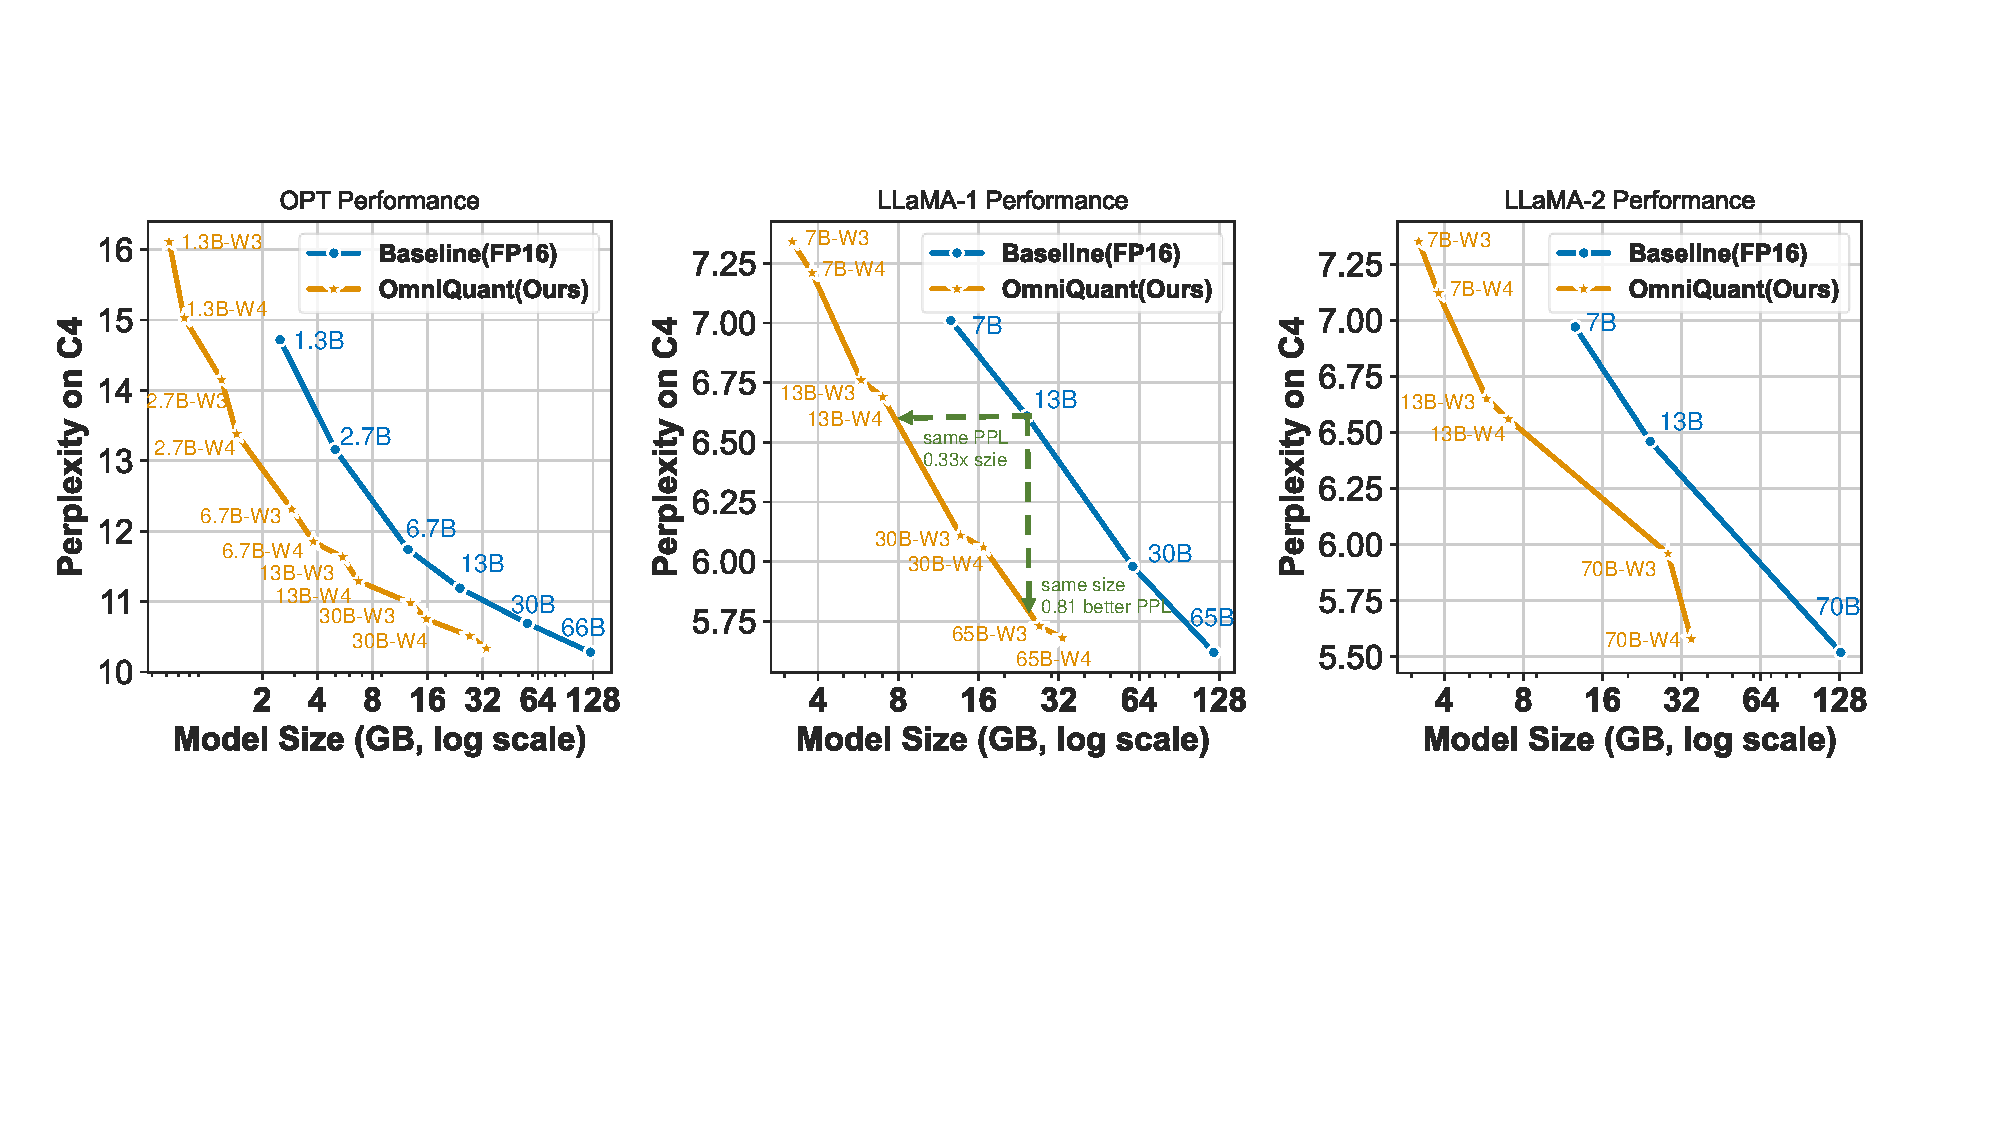
\includegraphics[width=0.95\textwidth]{performance_overview.pdf}
    \caption{\textbf{Performance overview.}  We display the trade-off curves for three model families. Each model showcases two quantization variants: W4A16g128 and W3A16g128. It is evident that OmniQuant markedly enhances the trade-off between perplexity and model size. Specifically, OmniQuant delivers a reduction of 0.81 in perplexity for an equivalent model size and achieves the same perplexity with only 0.33x of the model size.}
    \label{fig:performance_overview}
\end{figure}

% In this section, we present the full results on different dataset as a supplement of the main paper, including C4 perplexity for weight-only quantization in LLaMA families (Table\,\ref{tab:llama_weight_only_c4}), PTB perplexity for weight-only quantization in OPT families (Table\,\ref{tab:opt_weight_only_ptb}), C4 perplexity for weight-only quantization in OPT families (Table\,\ref{tab:opt_weight_only_c4}), WikiText2 perplexity for weight-activation quantization in LLaMA families (Table\,\ref{tab:llama_weight_activation_wiki}), and C4 perplexity for weight-activation quantization in LLaMA families (Table\,\ref{tab:llama_weight_activation_c4}).

\begin{table}[ht]
    \centering
    \caption{\textcolor{black}{\textbf{Average MMLU accuracy of LLaMa-7B.}}}
    \color{black}
    \begin{tabular}{ccccc}
    \hline
    LLaMa-1-7B (FP: 38.41\%) & W4A16g128 & W3A16g128 & W2A16g128 & W4A4 \\
    \hline
    RTN & 37.37\% & 33.43\% & 22.55\% & 23.31 \\
    GPTQ & 35.39\% & 30.53\% & 23.83\%  & - \\
    AWQ & \textbf{37.71\%} & 35.43\% & 22.58\% & - \\
    OP+ & - & - & - & 25.72 \\
    OmniQuant & 37.50\% & \textbf{35.60\%} & \textbf{26.03\%} & \textbf{26.93} \\
    \hline
    \end{tabular}
    \label{tab:mmlu}
\end{table}


\begin{table}[!ht]
\renewcommand{\arraystretch}{1.3}
\caption{Performance of weights and activations quantization on LLaMA-1-7B model with asymmetric bits.}
\centering
\resizebox{\linewidth}{!}{
\color{black}
\begin{tabular}{cccccccccccc}
\toprule
\multirow{2}{*}{\#Bits} & \multirow{2}{*}{Method} & \multicolumn{3}{c}{PPL $\downarrow$} & \multicolumn{7}{c}{Accuracy (\%) $\uparrow$} \\
\cmidrule(l{2pt}r{2pt}){3-5}
\cmidrule(l{2pt}r{2pt}){7-12}
& &  WikiText2 & C4 & Avg. & PIQA & ARC-e & ARC-c & BoolQ & HellaSwag & Winogrande & Avg. \\
\midrule
FP16 & - & 5.68 & 7.08 & 6.38 & 77.47  & 52.48 & 41.46 & 73.08 & 73.00 & 67.07 & 64.09 \\
W4A8 & OmniQuant & 5.87 & 7.34 & 6.60 & 77.36 & 51.85 & 38.65 & 70.67 & 71.20 & 64.71 & 62.40 \\
W4A6 & OmniQuant & 6.09 & 7.63 & 6.85 & 75.73 & 51.51 & 38.31 & 68.28 & 70.79 & 65.27 & 61.64 \\
W8A4 & OmniQuant & 10.27 & 12.77 & 11.52 & 69.47 & 45.87 & 32.84 & 59.08 & 58.66 & 54.85 & 53.46 \\
\bottomrule
\end{tabular}
}
\label{tab: asymmetric_bits}
\vspace{-0.15in}
\end{table}


\begin{table}[ht]
    \centering
    \setlength{\tabcolsep}{1pt}
    \caption{\textbf{Weight-only quantization on Falcon-180B.}}
    \resizebox{\linewidth}{!}{
    \begin{tabular}{ccccccccccccc}
    \hline
    \multicolumn{4}{c}{\textbf{Falcon-180b}} & \multicolumn{3}{c}{PPL$\downarrow$} & \multicolumn{6}{c}{Acc$\uparrow$} \\
    \cmidrule(l{2pt}r{2pt}){5-7}
    \cmidrule(l{2pt}r{2pt}){8-13} 
     Method & Bit\# &  Memory & Devices  & Wiki & PTB & C4 & PIQA  & ARC-e & Arc-c & BoolQ & HellaSwag & Winogrande \\
     \hline
     - & BF16/FP16 & 335GB & 5xA100 80GB & 3.29 & 6.64 & 6.31 & 84.82 & 84.20 & 60.83 & 86.85 & 85.91 & 80.58 \\
     RTN & W3A16g512 & 65GB & 1xA100 80GB & 5.33 & 8.08 & 8.34 & 83.48 & 80.85 & 55.46 & 78.37 & 81.05 & 77.97 \\
     \rowcolor{Gray} OmniQuant & W3A16g512 & \textbf{65GB} &  \textbf{1xA100 80GB} &  \textbf{3.71} &  \textbf{6.95} &  \textbf{6.71} &  \textbf{84.71} &  \textbf{82.91} &  \textbf{60.92} &  \textbf{84.03} &  \textbf{84.96} &  \textbf{79.40}\\
     \hline
    \end{tabular}
    }
    \label{tab:falcon-180b}
\end{table}



\begin{table}[!ht]
    \setlength{\tabcolsep}{8pt}
    \small
    \centering
    \caption{\textbf{C4 perplexity of Weight-only quantization results in LLaMA-1 and LLaMA-2 models} Continue of Table~\ref{tab:llama_weight_only}.}
    \label{tab:llama_weight_only_c4}
    \begin{tabular}{llccccccc}
        \hline
          \multicolumn{2}{l}{\textbf{LLaMA1\&2 / PPL}$\downarrow$} & 1-7B & 1-13B & 1-30B & 1-65B & 2-7B & 2-13B &2-70B \\  \hline
        FP16 & - & 7.08 & 6.61 & 5.98 & 5.62 & 6.97 & 6.46 & 5.52  \\ 
        \hline
        \multirow{3}{*}{\shortstack{W2A16}} & RTN & 1.3e5 & 5.6e4 & 2.7e4 & 2.2e4 & 4.8e4 & 7.2e4 & 2.4e4  \\
         & GPTQ  & 689.13 & 2.5e3  & 169.80 & 40.58 & NAN  & 323.12 & 48.82 \\
         & \cellcolor{Gray}\textbf{OmniQuant}  & \cellcolor{Gray}\textbf{24.89} & \cellcolor{Gray}\textbf{18.31} & \cellcolor{Gray}\textbf{13.89} & \cellcolor{Gray}\textbf{10.77} & \cellcolor{Gray}\textbf{90.64} & \cellcolor{Gray}\textbf{26.76} & \cellcolor{Gray}\textbf{12.28}   \\
        \hline
        \multirow{4}{*}{\shortstack{W2A16\\g128}} & RTN & 1.0e3 & 447.64 & 99.45 & 17.15 & 4.9e3 & 139.65 & 42.13  \\
         & GPTQ & 27.71 & 15.29 & 11.93 & 11.99 & 33.70 & 20.97 & NAN  \\
         & AWQ & 1.9e5 & 2.3e5 & 2.4e5 & 7.5e4 & 1.7e5 & 9.4e4 & -  \\
         & \cellcolor{Gray}\textbf{OmniQuant}  & \cellcolor{Gray}\textbf{12.97} & \cellcolor{Gray}\textbf{10.36} & \cellcolor{Gray}\textbf{9.36} & \cellcolor{Gray}\textbf{8.00} & \cellcolor{Gray}\textbf{15.02} & \cellcolor{Gray}\textbf{11.05} & \cellcolor{Gray}\textbf{8.52}   \\
        \hline
        \multirow{4}{*}{\shortstack{W2A16\\g64}} & RTN & 151.43 & 76.00 & 30.07 & 11.34 & 475.35 & 28.69 & 13.43  \\
         & GPTQ & 17.71 & 11.70 & 9.92 & 10.07 & 19.40 & 12.48 & NAN  \\
         & AWQ & 2.8e5 & 2.2e5 & 2.3e5 & 7.4e4 & 1.6e5 & 9.5e4 & -  \\
         & \cellcolor{Gray}\textbf{OmniQuant}  & \cellcolor{Gray}\textbf{11.78} & \cellcolor{Gray}\textbf{9.75} & \cellcolor{Gray}\textbf{8.65} & \cellcolor{Gray}\textbf{7.60} & \cellcolor{Gray}\textbf{12.72} & \cellcolor{Gray}\textbf{10.05} & \cellcolor{Gray}\textbf{7.88}   \\
         \hline
        \multirow{4}{*}{\shortstack{W3A16}} & RTN & 28.26 & 13.22 & 28.66 & 12.79 & 402.35 & 12.51 & 10.02  \\
         & GPTQ & 9.49 & 8.16 & 7.29 & 6.71 & 9.81 & 8.02 & 6.57  \\
         & AWQ & 13.26 & 9.13 & 12.67 & 7.11 & 23.85 & 13.07 & -  \\
         & \cellcolor{Gray}\textbf{OmniQuant} & \cellcolor{Gray}\textbf{8.19} & \cellcolor{Gray}\textbf{7.32} & \cellcolor{Gray}\textbf{6.57} & \cellcolor{Gray}\textbf{6.07} & \cellcolor{Gray}\textbf{8.65} & \cellcolor{Gray}\textbf{7.44} & \cellcolor{Gray}\textbf{6.06}   \\
         \hline
        \multirow{4}{*}{\shortstack{W3A16\\g128}} & RTN & 8.62 & 7.49 & 6.58 & 6.10 & 8.40 & 7.18 & 6.02  \\
         & GPTQ & 7.85 & 7.10 & 6.47 & 6.00 & 7.89 & 7.00 & 5.85  \\
         & AWQ & 7.92 & 7.07 & 6.37 & 5.94 & 7.84 & \textbf{6.94} & -  \\
         & \cellcolor{Gray}\textbf{OmniQuant}  & \cellcolor{Gray}\textbf{7.75} & \cellcolor{Gray}\textbf{7.05} & \cellcolor{Gray}\textbf{6.37} & \cellcolor{Gray}\textbf{5.93} & \cellcolor{Gray}\textbf{7.75} & \cellcolor{Gray}6.98 & \cellcolor{Gray}\textbf{5.85}   \\
         \hline
         \multirow{4}{*}{\shortstack{W4A16}} & RTN & 7.93 & 6.98 & 6.34 & 5.85 & 7.71 & 6.83 & 5.79  \\
         & GPTQ & 7.43 & 6.84 & 6.20 & 5.80 & 7.37 & 6.70 & 5.67  \\
         & AWQ & 7.52 & 6.86 & 6.17 & 5.77 & 7.68 & 6.74 & -  \\
         & \cellcolor{Gray}\textbf{OmniQuant}  & \cellcolor{Gray}\textbf{7.34} & \cellcolor{Gray}\textbf{6.76} & \cellcolor{Gray}\textbf{6.11} & \cellcolor{Gray}\textbf{5.73} & \cellcolor{Gray}\textbf{7.35} & \cellcolor{Gray}\textbf{6.65} & \cellcolor{Gray}\textbf{5.65}   \\
         \hline
         \multirow{4}{*}{\shortstack{W4A16\\g128}} & RTN & 7.37 & 6.69 & 6.06 & 5.69 & 7.24 & 6.58 & 5.63  \\
         & GPTQ & 7.21 & 6.69 & 6.06 & 5.69 & 7.12 & 6.56 & 5.58  \\
         & AWQ & 7.21 & 6.70 & 6.05 & 5.68 & 7.13 & 6.56 & -  \\
         & \cellcolor{Gray}\textbf{OmniQuant}  & \cellcolor{Gray}\textbf{7.21} & \cellcolor{Gray}\textbf{6.69} & \cellcolor{Gray}6.06 & \cellcolor{Gray}\textbf{5.68} & \cellcolor{Gray}\textbf{7.12} & \cellcolor{Gray}\textbf{6.56} & \cellcolor{Gray}\textbf{5.58}   \\
        \hline
    \end{tabular}
\end{table}

\begin{table}[!ht]
    \setlength{\tabcolsep}{5pt}
    \small
    \centering
    \caption{\textbf{WikiText2 perplexity of Weight-only quantization results in OPT models}.}
    \begin{tabular}{llccccccc}
        \hline
          \multicolumn{2}{l}{\textbf{OPT / PPL}$\downarrow$} & 125M  & 1.3B & 2.7B & 6.7B & 13B & 30B & 66B  \\  \hline
        FP16 & - & 27.65  & 14.63 & 12.47 & 10.86 & 10.12 & 9.56 & 9.34 \\ 
        \hline
        \multirow{4}{*}{\shortstack{W2A16\\g128}} & RTN & 7.2e3   & 1.3e4 & 5.7e4 & 7.8e3 & 7.6e4 & 1.3e4 & 3.6e5  \\
         & GPTQ &  597.66  & 115.16 & 61.59 & 20.18 & 21.36 &  12.71 & 82.10 \\
         & AWQ & 251.84  & 47.97 & 28.50 & 16.20 & 14.32 &  12.31 & 14.54   \\
         & \cellcolor{Gray}\textbf{OmniQuant}  & \cellcolor{Gray}\textbf{75.43}  & \cellcolor{Gray}\textbf{23.95} & \cellcolor{Gray}\textbf{18.13} & \cellcolor{Gray}\textbf{14.43} & \cellcolor{Gray}\textbf{12.94} & \cellcolor{Gray}\textbf{11.39} & \cellcolor{Gray}30.84  \\
        \hline
        \multirow{4}{*}{\shortstack{W2A16\\g64}} & RTN & 7.0e3  & 1.0e4 & 19.3e4 & 7.6e3 & 1.8e4 & 8.2e3 & 1.1e4  \\
         & GPTQ &  204.40 & 49.58 & 29.37 & 16.81 & 16.65 &  11.87 & 356.01 \\
         & AWQ & 124.18  & 29.78 & 20.64 & 14.63 & 13.28 &  11.59 & 12.74  \\
         & \cellcolor{Gray}\textbf{OmniQuant}  & \cellcolor{Gray}\textbf{62.56}  & \cellcolor{Gray}\textbf{21.40} & \cellcolor{Gray}\textbf{16.76} & \cellcolor{Gray}\textbf{13.57} & \cellcolor{Gray}\textbf{12.33} & \cellcolor{Gray}\textbf{11.00} & \cellcolor{Gray}\textbf{10.59}  \\ \hline
        \multirow{4}{*}{\shortstack{W3A16}} & RTN & 1.2e3  & 1.3e4 & 1.6e4 & 6.5e3 & 4.6e3 & 1.5e3 & 6.1 e3 \\
         & GPTQ &  53.05  & 21.17 & 16.83 & 15.09 & 11.73 &  10.30 & 14.42 \\
         & AWQ & 69.43 & 28.01 & 263.10 & 15.13 & 20.09 &  35.74 & 4.5e3  \\
         & \cellcolor{Gray}\textbf{OmniQuant}  & \cellcolor{Gray}\textbf{35.66} & \cellcolor{Gray}\textbf{16.68} & \cellcolor{Gray}\textbf{13.80} & \cellcolor{Gray}\textbf{11.65} & \cellcolor{Gray}\textbf{10.87} & \cellcolor{Gray}\textbf{10.00} & \cellcolor{Gray}\textbf{9.83}  \\ \hline
        \multirow{4}{*}{\shortstack{W3A16\\g128}} & RTN & 51.22  & 119.00 & 297.98 & 23.54 & 46.03 & 18.80 & 136.89w  \\
         & GPTQ &  39.24 & 16.47 & 13.69 & 11.65 & 10.35 &  9.73 & 10.96 \\
         & AWQ & 36.74 & 16.32 & 13.58 & 11.41 & 10.68 &  9.85 & 9.60  \\
         & \cellcolor{Gray}\textbf{OmniQuant}  & \cellcolor{Gray}\textbf{32.25} & \cellcolor{Gray}\textbf{15.72} & \cellcolor{Gray}\textbf{13.18} & \cellcolor{Gray}\textbf{11.27} & \cellcolor{Gray}\textbf{10.47} & \cellcolor{Gray}9.79 & \cellcolor{Gray}\textbf{9.53} \\ \hline
         \multirow{4}{*}{\shortstack{W4A16}} & RTN & 37.28 & 48.17 & 16.92 & 12.10 & 11.32 & 10.97 & 110 \\
         & GPTQ & 31.43 & 15.56 & 12.82 & 11.41 & 10.31 & 9.63 & 9.55 \\
         & AWQ & 32.28 & 15.49 & 12.93 & 11.30 & 10.39 &  9.77 & 9.61  \\
         & \cellcolor{Gray}\textbf{OmniQuant} & \cellcolor{Gray}\textbf{29.45} & \cellcolor{Gray}\textbf{15.04} & \cellcolor{Gray}\textbf{12.76} & \cellcolor{Gray}\textbf{11.03} &  \cellcolor{Gray}\textbf{10.30} & \cellcolor{Gray}9.65 & \cellcolor{Gray}9.65 \\ 
         \hline
         \multirow{4}{*}{\shortstack{W4A16\\g128}} & RTN & 30.47 & 15.29  & 13.02 & 11.15 & 10.30 & 9.94 & 9.65 \\
         & GPTQ & 29.81  & 14.89 & 12.52 & 10.93 & 10.17 & 9.58 & 9.34 \\
         & AWQ & 29.15  & 14.94 & 12.74 & 10.93 & 10.21 & 9.59 & 9.40 \\
         & \cellcolor{Gray}\textbf{OmniQuant} & \cellcolor{Gray}\textbf{28.86}   & \cellcolor{Gray}\textbf{14.88} & \cellcolor{Gray}12.65 & \cellcolor{Gray}\textbf{10.96} &  \cellcolor{Gray}10.20 & \cellcolor{Gray}9.62 &  \cellcolor{Gray}9.37 \\
        \hline
    \end{tabular}
    \label{tab:opt_weight_only_wiki}
\end{table}


\begin{table}[!ht]
    \setlength{\tabcolsep}{5pt}
    \small
    \centering
    \caption{\cellcolor{Gray}\textbf{PTB perplexity of Weight-only quantization results in OPT models}.}
    \begin{tabular}{llccccccc}
        \hline
          \multicolumn{2}{l}{\textbf{OPT / PPL}$\downarrow$} & 125M  & 1.3B & 2.7B & 6.7B & 13B & 30B & 66B  \\  \hline
        FP16 & - & 32.54 & 16.96  & 15.11 & 13.08  & 12.33 & 11.84 & 11.36 \\ 
        \hline
        \multirow{4}{*}{\shortstack{W2A16\\g128}} & RTN & 4.6e3  & 7.1e3 & 2.5e4 & 5.7e3 & 3.0e4 & 6.2e3 & 1.4e5  \\
         & GPTQ & 655.17  & 130.88 & 61.36 & 25.24 & 20.46 & 15.15 & 323.23 \\
         & AWQ & 263.88  & 71.87 & 43.15 & 19.49 & 17.61 & 14.92 & 19.33   \\
         & \cellcolor{Gray}\textbf{OmniQuant}  & \cellcolor{Gray}\textbf{126.49} & \cellcolor{Gray}\textbf{34.33} & \cellcolor{Gray}\textbf{25.28} & \cellcolor{Gray}\textbf{18.92} & \cellcolor{Gray}\textbf{16.74} & \cellcolor{Gray}\textbf{14.51} & \cellcolor{Gray}\textbf{139.17}  \\
        \hline
        \multirow{4}{*}{\shortstack{W2A16\\g64}} & RTN & 5.1e3  & 9.4e3 & 7.7e4 & 6.1e3 & 8.2e3 & 4.1e3 & 6.2e3  \\
         & GPTQ & 245.28  & 55.61 & 36.12 & 19.45 & 17.02 & 14.05 & 88.92 \\
         & AWQ   & 143.18 & 41.19 & 25.08 & 18.00 & 15.83 & 14.92 & 15.72   \\
         & \cellcolor{Gray}\textbf{OmniQuant}  & \cellcolor{Gray}\textbf{112.10} & \cellcolor{Gray}\textbf{30.36} & \cellcolor{Gray}\textbf{22.63} & \cellcolor{Gray}\textbf{17.58} & \cellcolor{Gray}\textbf{15.70} & \cellcolor{Gray}\textbf{13.98} & \cellcolor{Gray}\textbf{13.51}  \\
         \hline
        \multirow{4}{*}{\shortstack{W3A16}} & RTN & 1.2e3  & 1.1e4 & 1.0e4 & 5.2e3 & 3.6e3 & 1.4e3 & 3.6e3  \\
         & GPTQ & 34.05  & 27.39 & 15.94 & 13.75 & 13.71 & 12.54 & 21.16 \\
         & AWQ & 80.73  & 33.20 & 224.11 & 18.46 & 35.45 & 66.68 & 3.4e3   \\
         & \cellcolor{Gray}\textbf{OmniQuant}  & \cellcolor{Gray}\textbf{45.29} & \cellcolor{Gray}\textbf{20.42} & \cellcolor{Gray}\textbf{17.08} & \cellcolor{Gray}\textbf{14.23} & \cellcolor{Gray}\textbf{13.49} & \cellcolor{Gray}\textbf{12.54} & \cellcolor{Gray}\textbf{12.06}  \\
         \hline
        \multirow{4}{*}{\shortstack{W3A16\\g128}} & RTN & 64.67  & 222.13 & 337.75 & 39.90 & 65.33 & 34.27 & 309.69  \\
         & GPTQ & 45.17  & 19.90 & 17.06 & 14.24 & 12.84 & 12.54 & 13.27 \\
         & AWQ & 44.07  & 19.59 & 16.52 & 13.98 & 12.87 & 66.68 & 3.4e3   \\
         & \cellcolor{Gray}\textbf{OmniQuant}  & \cellcolor{Gray}\textbf{40.76} & \cellcolor{Gray}\textbf{19.06} & \cellcolor{Gray}\textbf{16.29} & \cellcolor{Gray}\textbf{13.77} & \cellcolor{Gray}\textbf{12.96} & \cellcolor{Gray}\textbf{12.19} & \cellcolor{Gray}\textbf{11.71}  \\
         \hline
         \multirow{4}{*}{\shortstack{W4A16}} & RTN & 44.98  & 33.63 & 22.23 & 16.05 & 15.40 & 14.17 & 274.23  \\
         & GPTQ & 37.75  & 18.23 & 15.94 & 13.75 & 12.58 & 11.98 & 11.58 \\
         & AWQ & 38.74  & 18.35 & 15.70 & 13.59 & 12.72 & 12.06 & 11.58   \\
         & \cellcolor{Gray}\textbf{OmniQuant}  & \cellcolor{Gray}\textbf{34.94} & \cellcolor{Gray}\textbf{17.80} & \cellcolor{Gray}\textbf{15.52} & \cellcolor{Gray}\textbf{13.41} & \cellcolor{Gray}\textbf{12.62} & \cellcolor{Gray}\textbf{11.95} & \cellcolor{Gray}\textbf{11.86}  \\
         \hline
         \multirow{4}{*}{\shortstack{W4A16\\g128}} & RTN & 36.50  & 33.63 & 22.23 & 16.05 & 15.40 & 14.17 & 11.79   \\
         & GPTQ & 35.48  & 17.41 & 15.42 & 13.21 & 12.42 & 11.89 & 11.51 \\
         & AWQ & 34.95  & 17.46 & 15.33 & 13.28 & 12.46 & 11.90 & 11.43   \\
         & \cellcolor{Gray}\textbf{OmniQuant}  & \cellcolor{Gray}\textbf{34.28} & \cellcolor{Gray}\textbf{17.40} & \cellcolor{Gray}\textbf{15.28} & \cellcolor{Gray}\textbf{13.25} & \cellcolor{Gray}\textbf{12.46} & \cellcolor{Gray}\textbf{11.94} & \cellcolor{Gray}\textbf{11.40}  \\
        \hline
    \end{tabular}
    \label{tab:opt_weight_only_ptb}
\end{table}

\begin{table}[!ht]
    \setlength{\tabcolsep}{5pt}
    \small
    \centering
    \caption{\textbf{C4 perplexity of Weight-only quantization results in OPT models}. }
    \begin{tabular}{llccccccc}
        \hline
          \multicolumn{2}{l}{\textbf{OPT / PPL}$\downarrow$} & 125M  & 1.3B & 2.7B & 6.7B & 13B & 30B & 66B  \\  \hline
        FP16 & - & 24.60  & 14.72 & 13.16 & 11.74 & 11.19 & 10.69 & 10.28 \\ 
        \hline
        \multirow{4}{*}{\shortstack{W2A16\\g128}} & RTN & 5.0e3  & 7.7e3 & 3.8e4 & 5.2e3 & 2.8e4 & 6.5e3 & 2.6e5  \\
         & GPTQ & 597.66  & 60.88 & 33.83 & 18.55 & 16.34 & 12.89 & 598.81 \\
         & AWQ & 168.35  & 38.38 & 26.41 & 16.48 & 14.73 & 12.98 & 15.42   \\
         & \cellcolor{Gray}\textbf{OmniQuant}  & \cellcolor{Gray}\textbf{80.10} & \cellcolor{Gray}\textbf{27.33} & \cellcolor{Gray}\textbf{21.11} & \cellcolor{Gray}\textbf{16.67} & \cellcolor{Gray}\textbf{14.92} & \cellcolor{Gray}\textbf{13.12} & \cellcolor{Gray}\textbf{73.83}  \\
        \hline
        \multirow{4}{*}{\shortstack{W2A16\\g64}} & RTN & 3.9e3  & 7.3e3 & 1.2e5 & 6.3e3 & 7.5e3 & 4.0e3 & 8.4e3  \\
         & GPTQ & 133.51  & 31.31 & 23.23 & 16.24 & 14.48 & 12.24 & 58.60 \\
         & AWQ & 90.19  & 27.34 & 20.01 & 15.20 & 13.90 & 12.43 & 13.31   \\
         & \cellcolor{Gray}\textbf{OmniQuant}  & \cellcolor{Gray}\textbf{64.01} & \cellcolor{Gray}\textbf{23.71} & \cellcolor{Gray}\textbf{19.16} & \cellcolor{Gray}\textbf{15.44} & \cellcolor{Gray}\textbf{14.16} & \cellcolor{Gray}\textbf{12.80} & \cellcolor{Gray}\textbf{12.13}   \\
         \hline
        \multirow{4}{*}{\shortstack{W3A16}} & RTN & 722.83  & 6.1e3 & 1.2e4 & 5.8e3 & 3.3e3 & 1.4e3 & 3.6e3  \\
         & GPTQ & 37.75  & 19.45 & 13.75 & 15.67 & 12.28 & 11.34 & 13.68 \\
         & AWQ & 55.73  & 24.56 & 154.49 & 15.84 & 23.71 & 55.01 & 3.8e3   \\
         & \cellcolor{Gray}\textbf{OmniQuant}  & \cellcolor{Gray}\textbf{32.17} & \cellcolor{Gray}\textbf{17.10} & \cellcolor{Gray}\textbf{14.93} & \cellcolor{Gray}\textbf{12.78} & \cellcolor{Gray}\textbf{12.13} & \cellcolor{Gray}\textbf{11.37} & \cellcolor{Gray}\textbf{10.82}  \\
         \hline
        \multirow{4}{*}{\shortstack{W3A16\\g128}} & RTN & 40.13  & 126.47 & 372.23 & 32.56 & 44.12 & 25.70 & 286.87  \\
         & GPTQ & 30.08  & 16.47 & 14.54 & 12.48 & 11.58 & 10.91 & 11.35 \\
         & AWQ & 30.39  & 16.27 & 14.19 & 12.30 & 11.61 & 10.96 & 10.53   \\
         & \cellcolor{Gray}\textbf{OmniQuant}  & \cellcolor{Gray}\textbf{29.34} & \cellcolor{Gray}\textbf{16.11} & \cellcolor{Gray}\textbf{14.15} & \cellcolor{Gray}\textbf{12.31} & \cellcolor{Gray}\textbf{11.63} & \cellcolor{Gray}\textbf{10.98} & \cellcolor{Gray}\textbf{10.51}  \\
         \hline
         \multirow{4}{*}{\shortstack{W4A16}} & RTN & 31.58  & 24.68 & 17.61 & 13.38 & 12.35 & 11.90 & 249.54  \\
         & GPTQ & 27.12  & 15.57 & 13.75 & 12.15 & 11.36 & 10.80 & 10.50 \\
         & AWQ & 27.64  & 15.65 & 13.71 & 12.04 & 11.42 & 10.83 & 10.41   \\
         & \cellcolor{Gray}\textbf{OmniQuant}  & \cellcolor{Gray}\textbf{26.36} & \cellcolor{Gray}\textbf{15.28} & \cellcolor{Gray}\textbf{13.58} & \cellcolor{Gray}\textbf{11.97} & \cellcolor{Gray}\textbf{11.41} & \cellcolor{Gray}\textbf{10.80} & \cellcolor{Gray}\textbf{10.63}  \\
         \hline
         \multirow{4}{*}{\shortstack{W4A16\\g128}} & RTN & 26.79  & 15.71 & 13.79 & 12.31 & 11.51 & 10.94 & 10.54  \\
         & GPTQ & 25.96  & 15.05 & 13.40 & 11.87 & 11.26 & 10.74 & 10.37 \\
         & AWQ & 25.90  & 15.04 & 13.39 & 11.87 & 11.28 & 10.75 & 10.34   \\
         & \cellcolor{Gray}\textbf{OmniQuant}  & \cellcolor{Gray}\textbf{25.63} & \cellcolor{Gray}\textbf{15.03} & \cellcolor{Gray}\textbf{13.38} & \cellcolor{Gray}\textbf{11.85} & \cellcolor{Gray}\textbf{11.29} & \cellcolor{Gray}\textbf{10.75}   & \cellcolor{Gray}\textbf{10.33} \\
        \hline
    \end{tabular}
    \label{tab:opt_weight_only_c4}
\end{table}


\begin{table}[!ht]
    \setlength{\tabcolsep}{8pt}
    \small
    \center
    \caption{\textbf{WikiText2 perplexity of weight-activation quantization results in LLaMA-1 and LLaMA-2 models} Continue of Table~\ref{tab:llama_weight_activation}.}
    \begin{tabular}{llccccccc}
        \hline
          \multicolumn{2}{l}{\textbf{LLaMA1\&2 / PPL}$\downarrow$} & 1-7B & 1-13B & 1-30B & 1-65B & 2-7B & 2-13B \\  \hline
        FP16 & - & 5.68 & 5.09 & 4.10 & 3.53 & 5.47 & 4.88   \\ 
        \hline
        \multirow{2}{*}{\shortstack{W6A6}} 
          & SmoothQuant & 6.03 & 5.42 & 4.55 & 3.88 & 6.20 & 5.18   \\
         & \cellcolor{Gray}\textbf{OmniQuant}  & \cellcolor{Gray}\textbf{5.96} & \cellcolor{Gray}\textbf{5.28} & \cellcolor{Gray}\textbf{4.38} & \cellcolor{Gray}\textbf{3.75} & \cellcolor{Gray}\textbf{5.87} & \cellcolor{Gray}\textbf{5.14}   \\
         \hline
        \multirow{2}{*}{\shortstack{W4A4}} 
          & SmoothQuant & 25.25 & 40.05 & 192.40 & 275.53 & 83.12 & 35.88   \\
         & \cellcolor{Gray}\textbf{OmniQuant}  & \cellcolor{Gray}\textbf{11.26} & \cellcolor{Gray}\textbf{10.87} & \cellcolor{Gray}\textbf{10.33} & \cellcolor{Gray}\textbf{9.17} & \cellcolor{Gray}\textbf{14.26} & \cellcolor{Gray}\textbf{12.30}   \\
        \hline
    \end{tabular}
    \label{tab:llama_weight_activation_wiki}
\end{table}


\begin{table}[!ht]
    \setlength{\tabcolsep}{8pt}
    \small
    \center
    \caption{\textbf{C4 perplexity of weight-activation quantization results in LLaMA-1 and LLaMA-2 models}. Continue of Table~\ref{tab:llama_weight_activation}.}
    \begin{tabular}{llcccccc}
        \hline
          \multicolumn{2}{l}{\textbf{LLaMA1\&2 / PPL}$\downarrow$} & 1-7B & 1-13B & 1-30B & 1-65B & 2-7B & 2-13B \\  \hline
        FP16 &  - & 7.08 & 6.61 & 5.98 & 5.62 & 6.97 & 6.46   \\ 
        \hline
        \multirow{2}{*}{\shortstack{W6A6}} 
          & SmoothQuant & 7.47 & 6.97 & 6.34 & 5.99 & 7.76 & 6,76   \\
         & \cellcolor{Gray}\textbf{OmniQuant}  & \cellcolor{Gray}\textbf{7.43} & \cellcolor{Gray}\textbf{6.84} & \cellcolor{Gray}\textbf{6.22} & \cellcolor{Gray}\textbf{5.82} & \cellcolor{Gray}\textbf{7.48} & \cellcolor{Gray}\textbf{6.74}   \\
         \hline
        \multirow{2}{*}{\shortstack{W4A4}} 
          & SmoothQuant & 32.32 & 47.18 & 122.38 & 244.35 & 77.27 & 43.19   \\
         & \cellcolor{Gray}\textbf{OmniQuant}  & \cellcolor{Gray}\textbf{14.51} & \cellcolor{Gray}\textbf{13.78} & \cellcolor{Gray}\textbf{12.49} & \cellcolor{Gray}\textbf{11.28}  & \cellcolor{Gray}\textbf{18.02} & \cellcolor{Gray}\textbf{14.55}  \\
        \hline
    \end{tabular}
    \label{tab:llama_weight_activation_c4}
\end{table}

\begin{table}[!ht]
\centering
\caption{ \textbf{Weight-activation quantization results of OPT Models.} We report perplexity on three datasets: WikiText2 (WIKI), Pen Treebank (PT), and C4. RPTQ indicates the data from RPTQ~(\cite{rptq}) paper, which keeps the output of LN and SoftMax as 8-bit. RPTQ$^*$ represents reproducing RPTQ with our setting that quantizes all activation into low-bit except keeping the softmax output at full precision. }
\label{tab:opt_weight_activation}
\resizebox{\linewidth}{!}{
\begin{tabular}{llcccccccccccc}
\hline
\multicolumn{2}{l}{\textbf{OPT / PPL}$\downarrow$}  & \multicolumn{3}{c}{OPT-6.7b} & \multicolumn{3}{c}{OPT-13b} & \multicolumn{3}{c}{OPT-30b} & \multicolumn{3}{c}{OPT-66b} \\ \hline
\multicolumn{2}{l}{Task}      & WIKI     & PT      & C4      & WIKI    & PT      & C4      & WIKI    & PT      & C4      & WIKI    & PT      & C4           \\ \hline
FP16   & -  & 10.86    & 13.09   & 11.74   & 10.13   & 12.34   & 11.20   & 9.56    & 11.84   & 10.69   & 9.34    & 11.36   & 10.28   \\
\hline
\multirow{4}{*}{\shortstack{W6A6}} & SmoothQuant & 11.34  & 13.82  & 12.14   & 10.56  & 12.76   & 11.40   & 9.67   & 12.01   & 10.81   & 10.72   & 13.25 & 11.60 \\
& RPTQ & 11.19  & 13.98  & 12.08   & 11.00  & 15.23   & 11.68   & 10.22   & 14.95   & 11.73   & 9.45   & 13.03 & 10.62 \\
& RPTQ$^*$ & 10.96  & 13.24  & 11.86   & 10.25  & 12.60   & 11.31   & 9.60   & 12.23   & 10.83   & 9.48   & 12.61 & 10.39 \\
& \cellcolor{Gray}\textbf{OmniQuant} & \cellcolor{Gray}\textbf{10.96}  & \cellcolor{Gray}\textbf{13.20}  & \cellcolor{Gray}\textbf{11.81}   & \cellcolor{Gray}\textbf{10.21}  & \cellcolor{Gray}\textbf{12.47}   & \cellcolor{Gray}\textbf{11.27}   & \cellcolor{Gray}\textbf{9.62}   & \cellcolor{Gray}\textbf{11.92}   & \cellcolor{Gray}\textbf{10.76}   & \cellcolor{Gray}\textbf{9.42}   & \cellcolor{Gray}\textbf{11.42}   & \cellcolor{Gray}\textbf{10.32}   \\   
\hline
\multirow{4}{*}{\shortstack{W4A4}} & SmoothQuant & 1.8e4  & 1.4e4  & 1.5e4   & 7.4e3  & 6.5e3   & 5.6e3   & 1.2e4   & 7.8e3   & 8.3e3   & 2.2e5   & 1.0e5 & 1.8e5 \\
 & RPTQ    & 12.00    & 15.17   & 12.85   & 12.74   & 15.76   & 14.71   & 11.15   & 14.11   & 13.48   & 12.23   & 18.87   & 15.93    \\
 & RPTQ$^*$    & 17.83    & 25.10   & 19.91   & 16.45  & 23.01   & 16.80   & 11.50   & 14.87   & 12.81  & 11.16   & 13.73   & 11.78    \\
& \cellcolor{Gray}\textbf{OmniQuant}   & \cellcolor{Gray}\textbf{12.24}  & \cellcolor{Gray}\textbf{15.54}  & \cellcolor{Gray}13.56   & \cellcolor{Gray}\textbf{11.65}  & \cellcolor{Gray}\textbf{15.89}   & \cellcolor{Gray}\textbf{13.46}   & \cellcolor{Gray}\textbf{10.60}   & \cellcolor{Gray}\textbf{13.75}   & \cellcolor{Gray}\textbf{11.89}   & \cellcolor{Gray}\textbf{10.29}   & \cellcolor{Gray}\textbf{13.19}   & \cellcolor{Gray}\textbf{11.35}   \\
\hline
\end{tabular}
}
\end{table}


% \begin{table}[]
%     \centering
%     \setlength{\tabcolsep}{1pt}
%     \resizebox{\linewidth}{!}{
%     \begin{tabular}{ccccccccccccc}
%     \hline
%     \multicolumn{4}{c}{\textbf{Falcon-180b}} & \multicolumn{3}{c}{PPL$\downarrow$} & \multicolumn{6}{c}{Acc$\uparrow$} \\
%     \cmidrule(l{2pt}r{2pt}){5-7}
%     \cmidrule(l{2pt}r{2pt}){8-13} 
%      Method & Bit\# &  Memory & Devices  & Wiki & PTB & C4 & PIQA  & ARC-e & Arc-c & BoolQ & HellaSwag & Winogrande \\
%      \hline
%      - & BF16/FP16 & 335GB & 5xA100 80GB & 3.29 & 6.64 & 6.31 & 84.82 & 84.20 & 60.83 & 86.85 & 85.91 & 80.58 \\
%      RTN & W3A16g512 & 65GB & 1xA100 80GB & 5.33 & 8.08 & 8.34 & 83.48 & 80.85 & 55.46 & 78.37 & 81.05 & 77.97 \\
%      \rowcolor{Gray} OmniQuant & W3A16g512 & \textbf{65GB} &  \textbf{1xA100 80GB} &  \textbf{3.71} &  \textbf{6.95} &  \textbf{6.71} &  \textbf{84.71} &  \textbf{82.91} &  \textbf{60.92} &  \textbf{84.03} &  \textbf{84.96} &  \textbf{79.40}\\
%      \hline
%     \end{tabular}
%     }
%     \caption{Weight-only quantization on Falcon-180B.}
%     \label{tab:my_label}
% \end{table}





\end{document}
